%% This is file `jcomp-template.tex',
%% 
%% Copyright 2017 Elsevier Ltd
%% 
%% This file is part of the 'Elsarticle Bundle'.
%% ---------------------------------------------
%% 
%% It may be distributed under the conditions of the LaTeX Project Public
%% License, either version 1.2 of this license or (at your option) any
%% later version.  The latest version of this license is in
%%    http://www.latex-project.org/lppl.txt
%% and version 1.2 or later is part of all distributions of LaTeX
%% version 1999/12/01 or later.
%% 
%% The list of all files belonging to the 'Elsarticle Bundle' is
%% given in the file `manifest.txt'.
%% 
%% Template article for Elsevier's document class `elsarticle'
%% with harvard style bibliographic references
%%
%% $Id: jcomp-template.tex 100 2017-07-14 13:15:12Z rishi $
%%
%% Use the option review to obtain double line spacing
%\documentclass[times,review,preprint,authoryear]{elsarticle}

%% Use the options `twocolumn,final' to obtain the final layout
%% Use longtitle option to break abstract to multiple pages if overfull.
%% For Review pdf (With double line spacing)
%\documentclass[times,twocolumn,review]{elsarticle}
%% For abstracts longer than one page.
%\documentclass[times,twocolumn,review,longtitle]{elsarticle}
%% For Review pdf without preprint line
%\documentclass[times,twocolumn,review,nopreprintline]{elsarticle}
%% Final pdf
\documentclass[times,final]{elsarticle}
%%
%\documentclass[times,twocolumn,final,longtitle]{elsarticle}
%%


%% Stylefile to load JCOMP template
\usepackage{jcomp}
\usepackage{framed,multirow}

%% The amssymb package provides various useful mathematical symbols
\usepackage{amssymb,amsmath}
\usepackage{latexsym}

% Following three lines are needed for this document.
% If you are not loading colors or url, then these are
% not required.
\usepackage{url}
%For \cellcolor
\usepackage[table]{xcolor}
\definecolor{newcolor}{rgb}{.8,.349,.1}
%Better boldface math font.
%\usepackage{bm}
\newcommand{\vr}{\vec{r}}
\newcommand{\vo}{\vec{\Omega}}
\usepackage{float}
\usepackage{subcaption}
\usepackage{placeins}
%%Algorithm
\usepackage{algorithm}
\usepackage{algorithmic}
%%For \ang
%\usepackage{siunitx}
%\newcommand{\jcr}[1]{\textcolor{red}{#1}}
%\usepackage[normalem]{ulem}
%\newcommand{\soutr}[1]{\jcr{\sout{#1}}}

\usepackage{color}
\newcommand{\tcr}[1]{\textcolor{red}{#1}}

\journal{Journal of Computational Physics}

%%%%%%%%%%%%%%%%%%%%%%%%%%%%%%%%%%%%%%%%%%%%%%%%%%%%%%%%%%%%%%%%%%%%%%%%%%%%%%%%%%%
\begin{document}
%%%%%%%%%%%%%%%%%%%%%%%%%%%%%%%%%%%%%%%%%%%%%%%%%%%%%%%%%%%%%%%%%%%%%%%%%%%%%%%%%%%

\verso{Given-name Surname \textit{etal}}

\begin{frontmatter}

\title{Choosing optimal partitions for massively parallel transport sweeps on unstructured grids}%\tnoteref{tnote1}}%
%\tnotetext[tnote1]{This is an example for title footnote coding.}

\author[1]{Tarek Habib \snm{Ghaddar}}%\corref{cor1}}
%\cortext[cor1]{Tarek Gahddar: 
%  Tel.: +0-000-000-0000;  
%  fax: +0-000-000-0000;}
\author[1]{Jean C. \snm{Ragusa}}
%\fntext[fn1]{This is author footnote for second author.}  

\address[1]{Department of Nuclear Engineering, Texas A\&M University, College Station, TX 77843, USA}

\received{1 May 2013}
\finalform{10 May 2013}
\accepted{13 May 2013}
\availableonline{15 May 2013}
\communicated{S. Sarkar}


%%%%%%%%%%%%%%%%%%%%%%%%%%%%%%%%%%%%%%%%%%%%%%%%%%%%%%%%%%%%%%%%%%%%%%%%%%%%%%%%%%%
\begin{abstract}
%%%%%%%%%%%%%%%%%%%%%%%%%%%%%%%%%%%%%%%%%%%%%%%%%%%%%%%%%%%%%%%%%%%%%%%%%%%%%%%%%%%
%%%
A concise and factual abstract is required. The abstract should state briefly the purpose of the research, the principal results and major conclusions. An abstract is often presented separately from the article, so it must be able to stand alone. For this reason, References should be avoided, but if essential, then cite the author(s) and year(s). Also, non-standard or uncommon abbreviations should be avoided, but if essential they must be defined at their first mention in the abstract itself.
%%%%
\end{abstract}

%\begin{keyword}
%% MSC codes here, in the form: \MSC code \sep code
%% or \MSC[2008] code \sep code (2000 is the default)
%\MSC 41A05\sep 41A10\sep 65D05\sep 65D17
%% Keywords
%\KWD Keyword1\sep Keyword2\sep Keyword3
%\end{keyword}

\end{frontmatter}

%\linenumbers

%%%%%%%%%%%%%%%%%%%%%%%%%%%%%%%%%%%%%%%%%%%%%%%%%%%%%%%%%%%%%%%%%%%%%%%%%%%%%%%%%%%
%%%%%%%%%%%%%%%%%%%%%%%%%%%%%%%%%%%%%%%%%%%%%%%%%%%%%%%%%%%%%%%%%%%%%%%%%%%%%%%%%%%
\section{Introduction}
%%%%%%%%%%%%%%%%%%%%%%%%%%%%%%%%%%%%%%%%%%%%%%%%%%%%%%%%%%%%%%%%%%%%%%%%%%%%%%%%%%%
%%%%%%%%%%%%%%%%%%%%%%%%%%%%%%%%%%%%%%%%%%%%%%%%%%%%%%%%%%%%%%%%%%%%%%%%%%%%%%%%%%%

The field of radiation transport studies the distribution of radiation (particle/energy) throughout a six-dimensional phase-space consisting of time, space, energy, and direction. 
Radiation transport is commonly used in reactor physics, medical physics, radiation shielding, criticality safety applications, stellar atmospheres, as well as the general simulation of radiation in different environments. 
Radiation transport is described by the Boltzmann transport equation \cite{bell_glasstone,zweifel,davison,duderstadt} and can be solved stochastically or deterministically.

The present papers deals with parallel solution techniques for the first-order form  of the $S_N$ transport equation. Hence, we consider the following discretizations of the transport equation: multigroup in energy, discrete-ordinates ($S_N$) in angle, and discontinuous finite elements in space. 
The resulting discrete system of equations is amenable to iterative techniques, whereby the streaming+total interaction operator need not to be assembled, generating large memory savings while being computationally very efficient.  
Essentially, this allows for a matrix-free approach, termed ``transport sweeps'' in the radiation transport community, where only small local systems of equations are solved cell-by-cell, for each angular direction and energy group, in a fashion that follows the flow of radiation in the computational mesh. After each transport sweep, the scattering source is updated and a new transport sweep is launched, an iterative process known as Source Iteration (SI). Alternatively to SI, the linear system can be recast of a sweep-preconditioned Krylov technique where, again, a transport sweep is necessary at each Krylov iteration.

In the past, extensive research has been done in parallelizing transport sweeps for structured grids and good parallel performance was achieved \cite{KBA,partisn,denovo,mpadams2013,mpadams2015,adamsJCP2000}. \tcr{you should have a brief overview of prior work, including KBA, PDT}
Partitioning unstructured grids for transport sweeps remains an open topic of research. \tcr{here, you should have a brief overview of prior unstructured grid work, including Pautz and your own MS work}. \tcr{These reviews are just provide the gyst of the ideas other researchers have followed. Like an elevator pitch, you need to go straight to the point, no digression, no details. If you elect to go deeper into prior methods, if they are important for your own work, this happens in early Sections, after the introduction}.
%Recently \cite{yourMSwork}, partitioning unstructured grids in a balanced fashion (i.e., with equivalent amounts of work per processor) can present challenges.

In the present the creation of distributed partitions must be amenable to   

The following sections will discuss a brief history of the transport sweep, parallel transport sweeps, load balancing unstructured meshes for transport, a time-to-solution estimator, and optimizing partitions for parallel transport.

Section \ref{cha:transport_sweeps} introduces the steady-state neutron transport equation and the discretization process to obtain the discrete form of the transport equation. Section \ref{cha:transport_sweeps} also provides more details on the transport sweep.

Massively parallel transport sweeps have been shown to scale up to 1.5 million cores on logically Cartesian grids using Texas A\&M's flagship deterministic transport code, PDT \cite{mpadams2013,mpadams2015}. \tcr{this has no place here. but that information should be moved up a bit}
Section \ref{cha:parallel_transport} describes the basics of a parallel sweep algorithm, and specifically describes the KBA algorithm \cite{KBA} and PDT's extension of the KBA algorithm.
This section also describes PDT's performance model, which predicts the sweep time given a set of partitioning parameters.

\tcr{OK, this is messed up. You cannot give a partial outline of the paper, then go back to talk about the backgroup, and then resume the outline. Please clean the introduction up}. In order to solve a wider set of problems, an unstructured meshing capability was implemented in PDT.
However, unstructured meshes may lead to imbalanced partitions, or different numbers of mesh cells per processor subdomain.
To address this, two load-balancing algorithms have been implemented in PDT, the original load-balancing algorithm and the load-balancing-by-dimension algorithm \cite{mastersthesis,mc2017}.

PDT's existing performance model does not account for unstructured meshes and imbalanced partitions.
Section \ref{cha:tts} describes the time-to-solution estimator, a graph-based method that estimates the time it takes to sweep across a problem given a mesh, partitioning scheme, and machine-specific parameters.

The time-to-solution estimator described in Section \ref{cha:tts} is used to optimize the partitioning scheme.
Section \ref{cha:optimization} details two optimization methods: a ``black box'' method that uses Python's scipy.optimize library and a ``human-intelligence'' method that prioritizes partition placement in locations that do not add cells to a mesh.

%%%%%%%%%%%%%%%%%%%%%%%%%%%%%%%%%%%%%%%%%%%%%%%%%%%%%%%%%%%%%%%%%%%%%%%%%%%%%%%%%%%
%%%%%%%%%%%%%%%%%%%%%%%%%%%%%%%%%%%%%%%%%%%%%%%%%%%%%%%%%%%%%%%%%%%%%%%%%%%%%%%%%%%
\section{Discretization of the transport equation}\label{cha:transport_sweeps}
%%%%%%%%%%%%%%%%%%%%%%%%%%%%%%%%%%%%%%%%%%%%%%%%%%%%%%%%%%%%%%%%%%%%%%%%%%%%%%%%%%%
%%%%%%%%%%%%%%%%%%%%%%%%%%%%%%%%%%%%%%%%%%%%%%%%%%%%%%%%%%%%%%%%%%%%%%%%%%%%%%%%%%%

\tcr{this is a paper. there is no need such so many details. I am taking a crack at shortening this part.\\}
The multigroup, steady-state neutron transport equation describing the distribution of neutral particles in a background medium is given by Eq.~\ref{multigroup}:
\begin{equation}
\vo \cdot \vec \nabla \psi_g(\vr,\vo) +\Sigma_{t,g}(\vr) \psi_g(\vr,\vo) = \frac{1}{4\pi}\sum_{g^{\prime}}\Sigma_{s,g^{\prime}\to g}(\vr)\phi_{g^{\prime}}(\vr) + S_{ext,g}(\vr,\vo), \quad \text{for } 1 \le g \le G
\label{multigroup}
\end{equation}
where $\vec{\Omega}\cdot \vec\nabla$ is the streaming operator and $\Sigma_{t,g}$ is the total interaction term in group $g$, $\psi_g(\vr,\vo)$ is the angular flux in group $g$. On the right-hand side, the scattering operator is present. Without loss of generality for the purpose of this paper, we limit ourselves to isotropic scattering for brevity. $S_{ext,g}$ is the external source. This forms a system of $G$ coupled transport equations. The scalar flux is defined as:
\begin{equation}
\label{def_scalar_flux}
\phi_g(\vr) = \int_{4\pi}d\Omega' \psi_g(\vr,\vo').
\end{equation}
Next, Eq.\eqref{multigroup} discretized in angle using the discrete ordinates ($S_N$) method \cite{miller_book}, whereby an angular quadrature $\left( \vo_m, w_m \right)_{1 \le m \le M}$ is used to solve the above equations along a given set of directions $\vo_m$:
\begin{equation}
\vo_m \cdot \vec \nabla \psi_{g,m}(\vr) +\Sigma_{t,g}(\vr) \psi_{g,m}(\vr)  = \frac{1}{4\pi}\sum_{g^{\prime}}\Sigma_{s,g^{\prime}\to g}(\vr)\phi_{g^{\prime}}(\vr) + S_{ext,g,m}(\vr),
\label{angle}
\end{equation}
where the subscript $m$ is introduced to denote the angular flux in direction $m$. Angular integration is replaced by a numerical quadrature
\begin{equation}
\label{def_scalar_flux_2}
\phi_g(\vr) \approx \sum_{m=1}^{m=M} w_m \psi_{g,m}(\vr).
\end{equation}
If one lags the evaluation of the scattering term in the right-hand side of Eq.\eqref{multigroup} (as in done, for instance, in the source iteration technique \cite{SI}), then it is apparent that the fundamental unit of work in solving the transport equation consists in being able to solve efficiently advection/reaction-type equations of the following form:
\begin{equation}
\vo_m \cdot \vec \nabla \psi_{m}^{(\ell+1)}(\vr) +\Sigma_{t}(\vr) \psi_{m}^{(\ell+1)}(\vr)  = \frac{1}{4\pi}\Sigma_{s}(\vr)\phi^{(\ell)}(\vr) + q^{ext}_m(\vr) = q_m(\vr),
\label{eq:one-group-transport}
\end{equation}
with $\ell$ the source iteration index.

After the energy and angular discretizations, Eq.~\eqref{eq:one-group-transport} is discretized in space. Here we employ discontinuous finite elements, which enables solving the transport problem of Eq.~\eqref{eq:one-group-transport} one cell at a time, flowing the flow of radiation in each direction $\vo_m$ (note that finite differences and finite volume techniques allows for transport sweeps too).
The solution across a cell interface is connected based on an upwind approach, where face outflow radiation becomes face inflow radiation for the downwind cells. Figure~\ref{sweeps} shows the sweep ordering for a given direction on both a structured and unstructured mesh.
\begin{figure}[H]
\centering
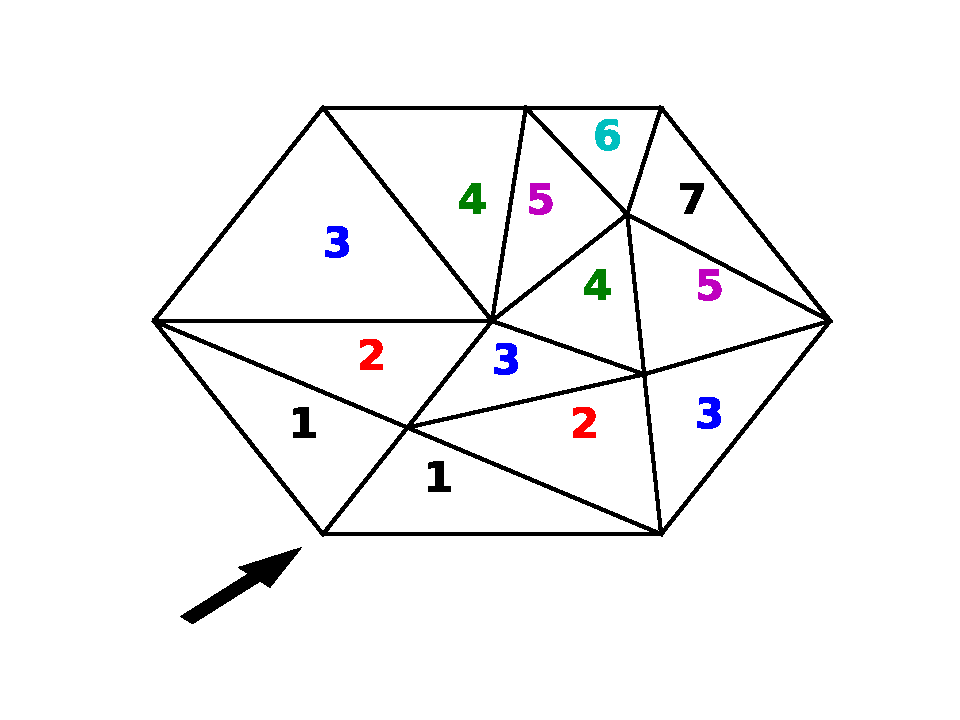
\includegraphics[scale=0.4]{../figures/UnstructuredMesh.pdf}
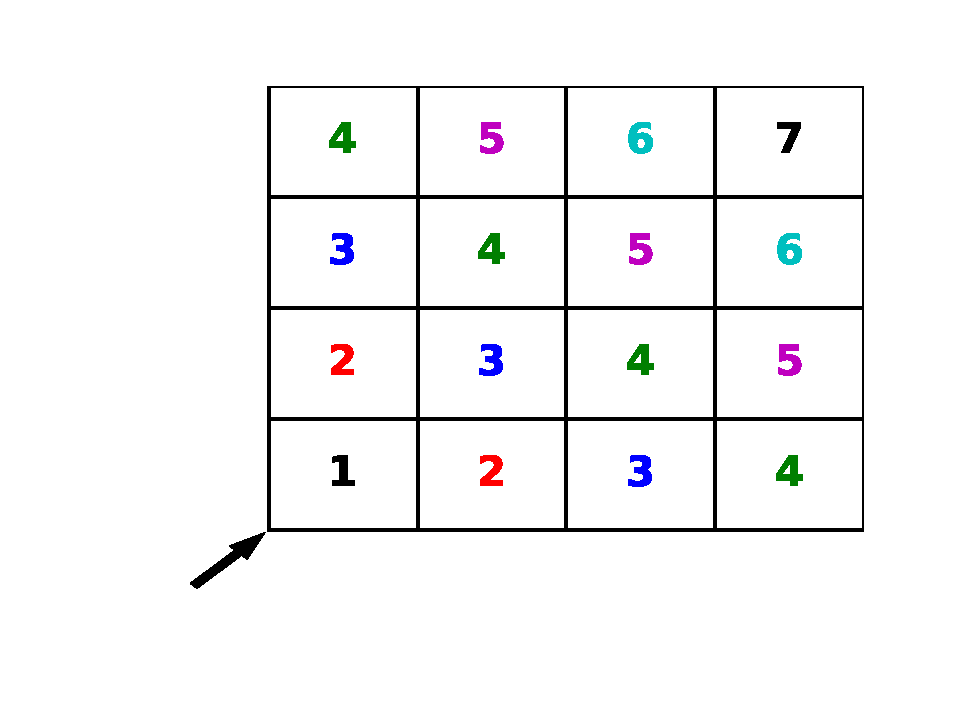
\includegraphics[scale = 0.4]{../figures/StructuredMesh.pdf}
\caption{A demonstration of a sweep on structured and unstructured meshes. The number in each cell represents the order in which the cells are solved.}
\label{sweeps}
\end{figure}
% All cells must receive the solution from downwind cells before their solution can be obtained.

\tcr{this should not be here in a paper but at the beginning of the next section}
The transport sweep can be parallelized in order to mitigate memory costs and obtain solutions in a reasonable time for large problems. Chapter \ref{cha:parallel_transport} describes the basics of a parallel sweep algorithm and details two algorithms: The KBA algorithm \cite{KBA} and PDT's extension of the KBA algorithm \cite{mpadams2013,mpadams2015,mpadamsjcp}.

%%%%%%%%%%%%%%%%%%%%%%%%%%%%%%%%%%%%%%%%%%%%%%%%%%%%%%%%%%%%%%%%%%%%%%%%%%%%%%%%%%%
%%%%%%%%%%%%%%%%%%%%%%%%%%%%%%%%%%%%%%%%%%%%%%%%%%%%%%%%%%%%%%%%%%%%%%%%%%%%%%%%%%%
\section{Parallel transport sweeps on structured grids}\label{cha:parallel_transport}
%%%%%%%%%%%%%%%%%%%%%%%%%%%%%%%%%%%%%%%%%%%%%%%%%%%%%%%%%%%%%%%%%%%%%%%%%%%%%%%%%%%
%%%%%%%%%%%%%%%%%%%%%%%%%%%%%%%%%%%%%%%%%%%%%%%%%%%%%%%%%%%%%%%%%%%%%%%%%%%%%%%%%%%
\tcr{everything from here all the way to Section 3.3 included needs to be severely reduced. You need to give the essence of what KBA partition is and PDT's extensions. It should be a detailed description, but clearly not as heavy as the one you have. currently, you have about 4 pages of text and almost 1 full page of figures. I think this should be reduced in a cohesive fashion to 1-1.5 pages of text and maybe no figures. Formulas are OK and defining terms that you will be using later is OK and recommended here but nothing beyond that as it will be superfluous.
Basically, I recommend the following sub-sections here:
\begin{enumerate}
\item General concepts that will make parallelization doable/feasible for transport sweeps. This is kind of a lay of the land and introduced+foreshadows the other subsections.
\item Example of the KBA algo
\item PDT's extension of KBA and comparison of both algos (similarities/improvements in PDT's). Maybe a bit of PDT's performance model.
\end{enumerate}
}

As mentioned in Chapter \ref{cha:transport_sweeps}, a transport sweep is set up by overlaying a domain with a finite element mesh and solving the transport equation cell by cell using a discontinuous finite element approach. A transport sweep can be solved in parallel in order to obtain the solution faster, as well as distribute the problem across many processors for memory intensive problems.

In PDT, a transport sweep can be performed on a structured Cartesian or arbitrary polyhedral mesh. Sweeping on an unstructured mesh presents two challenges: maintaining sweep efficiency on a massively parallel scale and keeping non-concave sub-domains to avoid cycles. PDT has already proven the ability to perform massively parallel transport sweeps on structured meshes. As part of previous efforts in PDT, researchers have outlined three important properties for parallel sweeps.

A parallel sweep algorithm is defined by three properties \cite{mpadams2013} :
\begin{itemize}
\item partitioning: dividing the domain among available processors,
\item aggregation: grouping cells, directions, and energy groups into tasks,
\item scheduling: choosing which task to execute if more than one is available.
\end{itemize}
It is important to note that these properties apply after any cell-level cycles are broken, but partitioning can introduce cycles between processors.

The basic concepts of parallel transport sweeps, partitioning, aggregation, and scheduling, are most easily described in the context of a  transport sweep that takes place on a structured Cartesian mesh. Furthermore, the work detailed in Chapters \ref{cha:lb} and \ref{cha:tts} utilize aspects of the structured transport sweep.

In a regular grid, we have the  number of cells in each Cartesian direction: $N_x, N_y, N_z$. These cells are aggregated into ``cellsets'', using aggregation factors $A_x, A_y, A_z$. If $M$ is the number of angular directions per octant, $G$ is the total number of energy groups, and $N$ is the total number of cells, then the total fine-grain work units is $8MGN$. The factor of 8 is present as $M$ directions are swept for all 8 octants. We often discuss the directions in a sweep in terms of octant-pairs, or two octants that have opposing sweep ordering. This is an important concept that is discussed in Section \ref{sec:KBA}. The finest-grain work unit is the calculation of a single direction and energy group's unknowns in a single cell, or $\psi_{m,g}$ for a single cell.

Fine-grain work units are aggregated into coarser-grained units called \textit{tasks}. A few terms are defined that describe how each variable is aggregated.
\begin{itemize}
\item $A_x = \frac{N_x}{P_x}$, where $N_x$ is the number of cells in $x$ and $P_x$ is the number of processors in $x$.
\item $A_y = \frac{N_y}{P_y}$, where $N_y$ is the number of cells in $y$ and $P_y$ is the number of processors in $y$.
\item $A_z$ = a selectable number of z-planes of $A_x A_y$ cells.
\item $N_g = \frac{G}{A_g}$
\item $N_m = \frac{M}{A_m}$
\item $N_k = \frac{N_z}{P_z A_z}$
\item $N_k A_x A_y A_z = \frac{N_x N_y N_z}{P_x P_y P_z}$
\end{itemize}

It follows that each process owns $N_k$ cellsets (each of which is $A_z$ planes of $A_x A_y$ cells), $8N_m$ angle-sets, and $N_g$ group-sets for a total of $8N_m N_g N_k$ tasks.

One task contains $A_x A_y A_z$ cells, $A_m$ directions, and $A_g$ groups. Equivalently, a task is the computation of one cellset, one groupset, and one angleset, with the completion of one task defined as a stage.  The stage is particularly important when assessing sweeps against analytical performance models.
Equation ~\ref{paralleleff} defines parallel sweep efficiency:
\begin{equation}\label{paralleleff}
\begin{split}
\epsilon &= \frac{T_{\text{task}} N_{\text{tasks}}}{[N_{\text{stages}}] [T_{\text{task}} + T_{\text{comm}}]} \\
            &=\frac{1}{[1+\frac{N_{\text{idle}}}{N_{\text{tasks}}}][1 + \frac{T_{\text{comm}}}{T_{\text{task}}}]},
\end{split}
\end{equation}
where $N_\text{idle}$ is the number of idle stages per processor, $N_\text{tasks}$ is the number of tasks each processor performs, $T_\text{comm}$ is the time to communicate after completion of a task, and $T_\text{task}$ is the time it takes to compute one task.
Equations ~\ref{Tcomm} and ~\ref{Ttask} show how $T_{\text{comm}}$ and $T_{\text{task}}$ are calculated:
\begin{align}
T_{\text{comm}} &= M_L T_{\text{latency}} + T_{\text{byte}} N_{\text{bytes}}, \\
N_{\text{bytes}} &= (A_x A_y + A_x A_z + A_y A_z)A_g A_m upbc,
\label{Tcomm}
\end{align}
\begin{equation}
T_{\text{task}} = A_x A_y A_z A_m A_g T_{\text{grind}},
\label{Ttask}
\end{equation}
where $T_{\text{latency}}$ is the message latency time, $T_{\text{byte}}$ is the time required to send one byte of message, $N_{\text{bytes}}$ is the total number of bytes of information that a processor must communicate to its downstream neighbors at each stage, $upbc$ is the unknowns per boundary cell (generally 2 for 2D and 4 for 3D) and $T_{\text{grind}}$ is the time it takes to compute a single cell, direction, and energy group. $M_L$ is a latency parameter that is used to explore performance as a function of increased or decreased latency. Note that Eq. \ref{Ttask} is idealized as it does not take into account overhead in various parts of the sweep implementation.

Before expanding on the proposed method of partitioning and scheduling for parallel transport sweeps, a quick review of two parallel transport sweep algorithms is necessary. This dissertation's method will expand on PDT's sweep algorithm \cite{mpadams2013,mpadams2015,mpadamsjcp}, which is an extension of the popular KBA algorithm \cite{KBA}.

%%%%%%%%%%%%%%%%%%%%%%%%%%%%%%%%%%%%%%%%%%%%%%%%%%%%%%%%%%%%%%%%%%%%%%%%%%%%%%%%%%%
\subsection{The KBA Algorithm}\label{sec:KBA}
%%%%%%%%%%%%%%%%%%%%%%%%%%%%%%%%%%%%%%%%%%%%%%%%%%%%%%%%%%%%%%%%%%%%%%%%%%%%%%%%%%%

Several parallel transport sweep codes use KBA partitioning in their sweeping, such as Denovo \cite{denovo} and PARTISN \cite{partisn}. The KBA partitioning scheme and algorithm was developed by Koch, Baker, and Alcouffe \cite{KBA}.

The KBA algorithm traditionally chooses $P_z = 1, A_m = 1 \text{ (or 1 angle per angleset)}, G = A_g = 1, A_x = N_x/P_x, A_y = N_y/P_y$, with $A_z$ being the selectable number of z-planes to be aggregated into each task. This partitions the domain into long, thin columns. With $N_k = N_z/A_z$, each processor performs $N_{\text{tasks}} = 8MN_k$ tasks. The KBA algorithm traditionally solves a problem one energy group at a time, and uses a ``pipelining'' or assembly line approach. This allows for new angles in an octant to begin sweeping before old angles have fully swept across the spatial domain. Figure~\ref{pipeline_example} shows an example of pipelining the angular work of a quadrant.
Figure~\ref{pipeline_example_3d} shows pipelining in the X-Z plane with $A_z = 1$.

\begin{figure}[h]
\centering
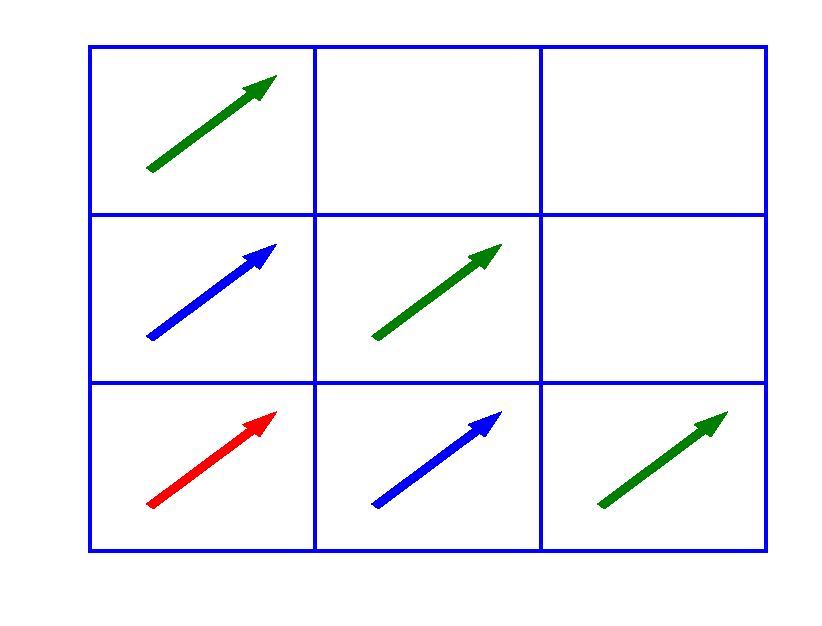
\includegraphics[scale=0.7]{../figures/pipeline_example.pdf}
\caption{An example showing the pipelining of angular work from the lower left quadrant.}
\label{pipeline_example}
\end{figure}
\begin{figure}[h]
\centering
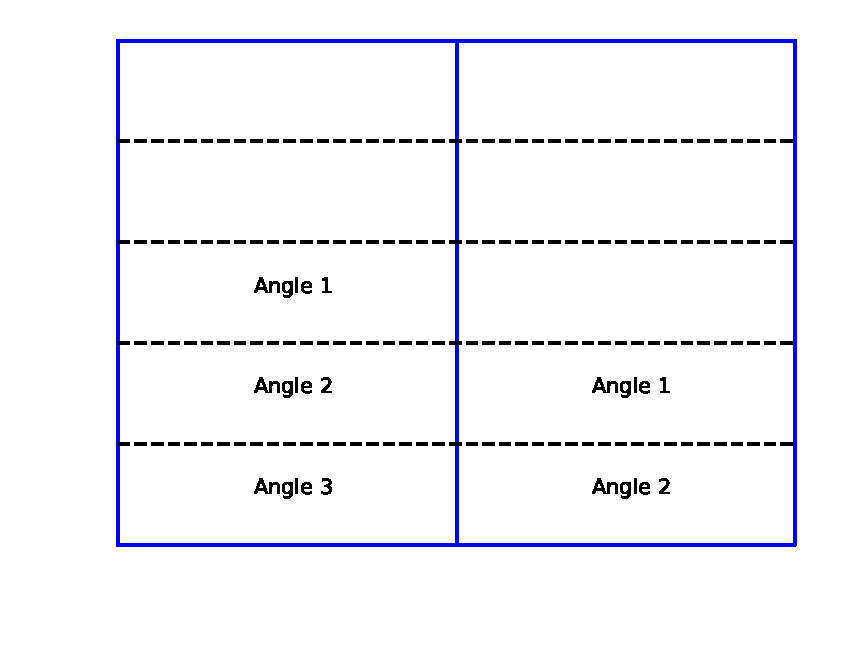
\includegraphics[scale=0.7,trim={0cm 1cm 0cm 0cm},clip]{../figures/pipeline_example_3d.pdf}
\caption{An example showing pipelining in the X-Z plane with $A_z = 1$, $P_x = 2$ and $P_z = 1$.}
\label{pipeline_example_3d}
\end{figure}

In Fig.~\ref{pipeline_example}, each square represents a processor that owns a group of $A_xA_y$ cells. We see that as soon as a processor is free to solve the next angle with the same sweep ordering, it begins immediately.
Figure~\ref{pipeline_example_3d} shows us the X-Z plane of a processor layout with $P_x = 2$ and $P_z = 1$. We see $N_k=\frac{N_z = 5}{A_z = 1}=5$ planes in Z, and three angles pipelined. We notice as soon as a cellset of $A_xA_yA_z$ cells is free to solve the next angle with the same sweep ordering, it begins immediately.
KBA introduced pipelining in order to combat the inherent inefficiencies of waiting for all processors to complete a sweep in a direction before starting the next angle.

There are two variants to the KBA algorithm, ``successive in angle, successive in quadrant", and ``simultaneous in angle, successive in quadrant".  With ``successive in angle, successive in quadrant", an octant pipelines its angular work, and once all directions are complete the opposing octant pipelines them back. This is then done for the remaining octant pairs. With ``simultaneous in angle, successive in quadrant", all angles from one octant are aggregated and solved rather than pipelined, and upon completion the opposing octant solves them. This is done either by aggregating angles, This is then done for the remaining octant pairs. The KBA parallel efficiency \cite{mpadams2013} for ``successive in angle, successive in quadrant" is:
\begin{equation}
  \epsilon_{KBA} = \frac{1}{[1 + \frac{4(P_x+P_y-2)}{8MN_k}][1 + \frac{T_{\text{comm}}}{T_{\text{{task}}}}]}.
  \label{eps_kba}
\end{equation}
The KBA parallel efficiency for ``simultaneous in angle, successive in quadrant'' is:
\begin{equation}
   \epsilon_{KBA} = \frac{1}{[1 + \frac{4(P_x+P_y-2)}{8MN_k/(A_m)}][1 + \frac{T_{\text{comm}}}{T_{\text{{task}}}}]}.
   \label{eps_kba_simul}
\end{equation}
For each octant-pair, the idle time is $P_x + P_y - 2$, and if the successive octant-pairs don't start until the previous octant pair finishes, then the total idle time is $4(P_x + P_y - 2)$.

%%%%%%%%%%%%%%%%%%%%%%%%%%%%%%%%%%%%%%%%%%%%%%%%%%%%%%%%%%%%%%%%%%%%%%%%%%%%%%%%%%%
\subsection{PDT's Extension of KBA}\label {pdt_extension}
%%%%%%%%%%%%%%%%%%%%%%%%%%%%%%%%%%%%%%%%%%%%%%%%%%%%%%%%%%%%%%%%%%%%%%%%%%%%%%%%%%%

PDT's extension of KBA does not limit $P_z, A_m, G,$ or $A_g$. In addition, all 8 octants (4 quadrants in 2D) begin work immediately. Unlike KBA, PDT's scheduling requires conflict resolution in its algorithm, as the pipelines from all octants will end up colliding toward the middle of the processor domain.

If two or more tasks reach a processor at the same time, PDT employs a tie breaking strategy:

\begin{enumerate}
	\item The task with the greater depth-of-graph remaining (simply, more work remaining) goes first.
	\item If the depth-of-graph remaining is tied, then octant-priority tie-breaking is used:
	\begin{enumerate}
	  \item The task with $\Omega_x > 0$ wins.
	  \item If multiple tasks have $\Omega_x > 0$, then the task with $\Omega_y > 0$ wins.
	  \item If multiple tasks have $\Omega_y > 0$, then the task with $\Omega_z > 0$ wins.
	\end{enumerate}
\end{enumerate}

Given these conflict resolution techniques, the minimum possible number of stages for given partitioning parameters $P_i$ and $A_j$ is $2N_{\text{fill}} + N_{\text{tasks}}$. $N_{\text{fill}}$ is both the minimum number of stages before a sweepfront can reach the center-most processors and the number needed to finish a direction's sweep after the center-most processors have finished. Equations \ref{nfill}, \ref{nidle}, and \ref{ntasks} define $N_{\text{fill}}, N_{\text{idle}}$, and $N_{\text{tasks}}$:

\begin{align}
N_\text{fill} = \frac{P_x + \delta_x}{2} - 1 + \frac{P_y + \delta_y}{2} - 1 + N_k (\frac{P_z + \delta_z}{2} - 1)\label{nfill} \\
\delta_u = 0 \text{ or } 1 \text{ for $P_u$ even or odd, respectively} \nonumber
\end{align}
\begin{equation}
N_\text{idle} = 2N_{\text{fill}}
\label{nidle}
\end{equation}
\begin{equation}
N_\text{tasks} = 8N_mN_gN_k
\label{ntasks}
\end{equation}
Plugging these definitions into Eq. \ref{paralleleff}, the PDT optimal parallel efficiency \cite{mpadams2013} for $P_u$ even is:
\begin{equation}
	\epsilon_{opt} = \frac{1}{ [1 + \frac{P_x + P_y - 4 + N_k(P_z -2)}{8MGN_k/(A_m A_G)} ]  [ 1 +  \frac{T_{\text{comm}}}{T_{\text{task}}} ]}
	\label{eps_opt}
\end{equation}

Let us consider how many more processors the hybrid partitioning with optimal scheduling ($P_z = 2$) can use while yielding the same efficiency as KBA.
Consider the limit of a large number of processors for both KBA and hybrid partioning with an optimal schedule.
Equation \ref{large_p_kba} shows the KBA efficiency in the large-P limit with $P_x + P_y \approx 2P^{1/2}$.
Setting $A_m = A_g = 1$ to match traditional KBA aggregation parameters, Eq. \ref{large_p_opt} shows the hybrid optimal efficiency in the large-P limit with $P_z = 2$ and $P_x + P_y \approx 2P^{1/2}$.
\begin{equation}
  \epsilon_{KBA} \xrightarrow{\text{large P}} \frac{1}{[1 + \frac{(4P^{1/2})}{8MN_k}][ 1 +  \frac{T_{\text{comm}}}{T_{\text{task}}}]}
  \label{large_p_kba}
\end{equation}
\begin{equation}
  \epsilon_{opt,hybrid} \xrightarrow{\text{large P}} \frac{1}{[1 + \frac{\sqrt{2}P^{1/2}}{8MN_k}][ 1 +  \frac{T_{\text{comm}}}{T_{\text{task}}} ]}
  \label{large_p_opt}
\end{equation}

If we set Eq. \ref{large_p_kba} equal to Eq. \ref{large_p_opt}, we see that in the limit of a large number of processors $P$, the optimal algorithm yields the same efficiency as KBA with 32 times as many processors \cite{mpadams2013, mpadams2015,mpadamsjcp}.

%%%%%%%%%%%%%%%%%%%%%%%%%%%%%%%%%%%%%%%%%%%%%%%%%%%%%%%%%%%%%%%%%%%%%%%%%%%%%%%%%%%
\subsection{PDT's Performance Model}
%%%%%%%%%%%%%%%%%%%%%%%%%%%%%%%%%%%%%%%%%%%%%%%%%%%%%%%%%%%%%%%%%%%%%%%%%%%%%%%%%%%

To aid in the selection of optimal processor and aggregation parameters, PDT uses a performance model to estimate the sweep time.
This performance model is the basis for the cost function described in Chapter \ref{cha:tts}.
Equation \ref{sweep_time} calculates the sweep time by multiplying the time it takes to solve each stage by the number of stages. This is then multiplied by a multi-core fudge factor that estimates the performance drop-off from 1 to 8 cores due to parallel overhead.
\begin{equation}
\text{Sweep Time} = \text{mcff}\cdot[\text{num stages}\cdot(T_{wu} + 3\cdot \text{latency}\cdot M_L + T_{\text{byte}}\cdot N_{\text{bytes}} + N_{\text{cells}}\cdot ( T_c +  A_m\cdot (T_m + T_g)))],
\label{sweep_time}
\end{equation}
where:
\begin{itemize}
  \item mcff = the Multi-Core Fudge Factor, a corrective factor that accounts for performance drop-off from 1 to 8 cores,
  \item num stages = tasks per processor + $2N_{\text{idle}}$,
  \item tasks per processor = $\frac{N_x}{P_x A_x} \frac{N_y}{P_y A_y} \frac{N_z}{P_z A_z} \frac{N_m}{A_m} \frac{N_g}{A_g}$,
  \item $T_{wu}$ = the time to get into the sweep operator,
  \item latency = the machine specific communication latency,
  \item $M_L$ = the machine specific latency multiplier,
  \item $T_{\text{byte}}$ = the communication time per double,
  \item $N_{\text{byte}}$ = the bytes per 3 communications (assuming 3 neighbors) = $(A_x A_y + A_x A_z + A_y A_z)A_g A_m upbc $,
  \item $upbc$ = unknowns per boundary cell (4 for 3d, 2 for 2d),
  \item $N_{\text{cells}}$ = the number of cells per task, $A_x A_y A_z$,
  \item $T_c$ = the time spent solving cell-specific work,
  \item $T_m$ = the time spent solving angle-specific work,
  \item $T_g$ = the time spent solving group-specific work.
\end{itemize}

A comparison between this performance model and the time-to-solution estimator will be shown in Chapter \ref{cha:tts}. Before this, we motivate the need for the time-to-solution estimator in Chapter \ref{cha:lb} by describing unstructured meshes in PDT and how we load balance them.

%%%%%%%%%%%%%%%%%%%%%%%%%%%%%%%%%%%%%%%%%%%%%%%%%%%%%%%%%%%%%%%%%%%%%%%%%%%%%%%%%%%
\subsection{Evaluation of existing partitioning strategies for parallel transport sweeps in unstructured grids}\label{cha:lb}
%%%%%%%%%%%%%%%%%%%%%%%%%%%%%%%%%%%%%%%%%%%%%%%%%%%%%%%%%%%%%%%%%%%%%%%%%%%%%%%%%%%
\tcr{Starting here, I think you should started a new Section. It should have the following subsections:
\begin{enumerate}
\item General ideas of how PDT's does its unstructured grid partitioning. This is kind of a lay of the land and introduced+foreshadows the other subsections.
\item Principle of mesh cutting for the purposes of parallel partitioning. 
\item Current load balancing strategies (LB and LBD -due to issues with standard LB). You have some numerical examples so maybe a few can stay here.
\end{enumerate}
I think this should be no more than 5-6 pages. Currently, from 3.4 until section 4 (excluded), you have 11 pages.
}
 
Initially, PDT only swept on structured, logically Cartesian meshes. As the need to solve problems with more complex geometries arose, PDT added a support for arbitrary polyhedral unstructured meshes. However, this introduced imbalanced partitions (or different amounts of cells per processor), causing longer and unmanageable runtimes.

To combat imbalanced partitions, two load balancing algorithms were implemented, referred to in this thesis as the original load-balancing algorithm \cite{mastersthesis,mc2017} and the load-balancing-by-dimension algorithm.

Before detailing the two load balancing algorithms PDT employs, a quick review of partitioning unstructured meshes in PDT is necessary:
\begin{itemize}
\item ``Cut lines'' in 2D (``cut planes'' in 3D) are used to slice through the mesh in the $x$, $y$, and $z$ dimensions.
\item The cut planes form brick partitions, called subsets, that have unstructured meshes inside of them.
\item Discontinuities along subset boundaries are fixed by ``stitching'' hanging nodes, creating degenerate polygons along subset boundaries.
\item The subsets are distributed amongst the processor domain.
\end{itemize}
Using cut lines/cut planes to partition unstructured meshes may preserve the provably optimal sweep partitioning \cite{mpadams2013,mpadams2015,mpadamsjcp} of logically Cartesian grids if each partition has an equivalent number of cells.
Subsets, rather than the cells, have $(i,j,k)$ indices and will become the base unit when aggregating spatial parameters. That is, $A_x$ and $A_y$ will now represent the number of subsets in $x$ and $y$ aggregated into a task.
Generally, one subset is assigned per processor, as this minimizes the communication costs across processor boundaries, although this is not required.
Figure~\ref{partitioning_example} shows an example of an unstructured mesh partitioned into 100 subsets in PDT.
\begin{figure}[H]
\centering
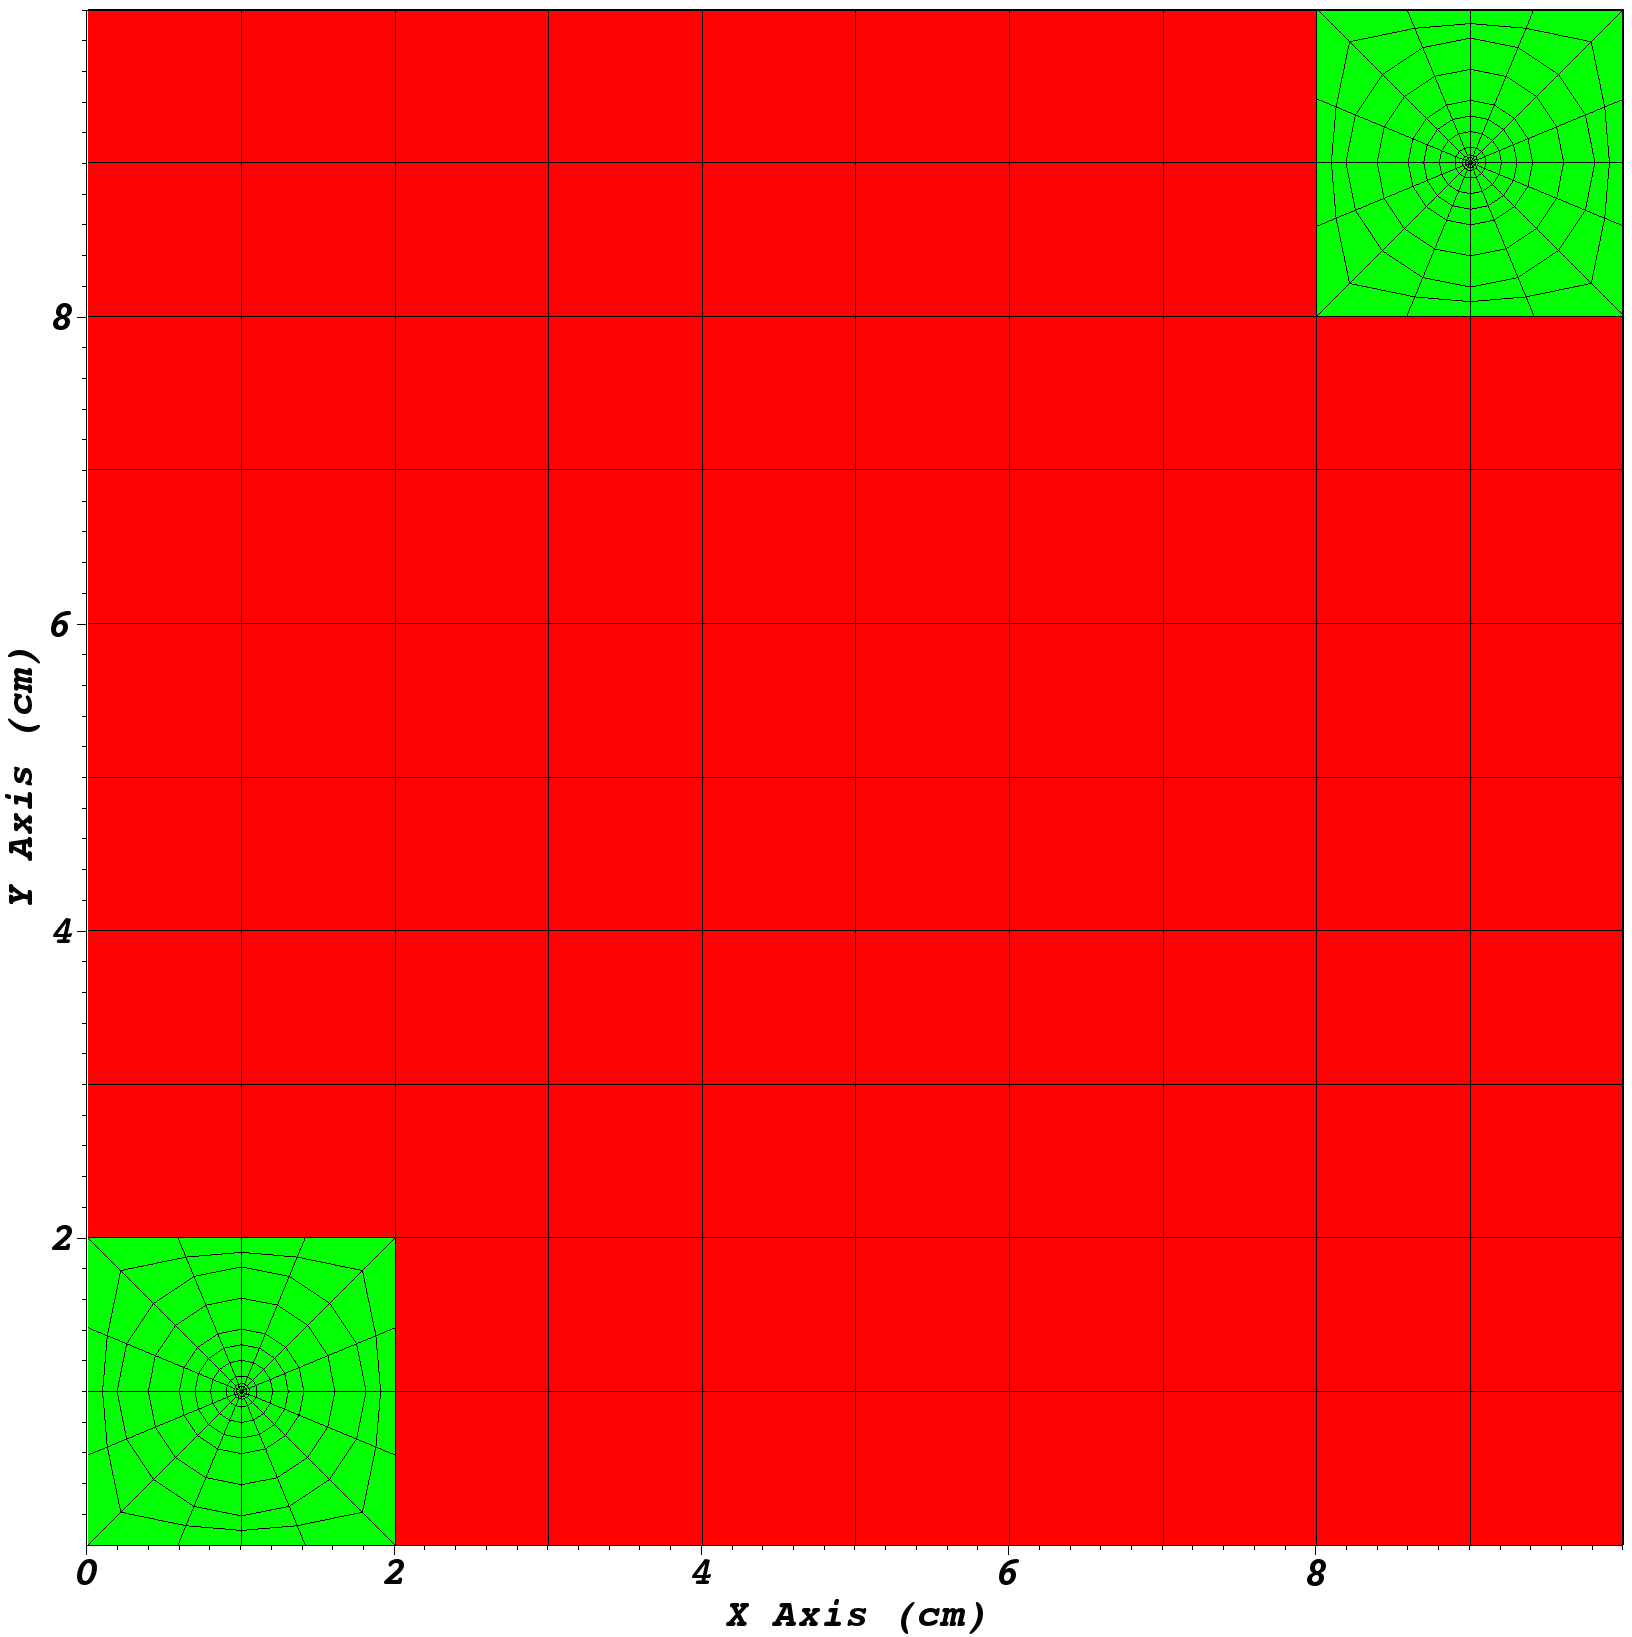
\includegraphics[scale=0.2]{../figures/spiderweb_10x10_sparse.png}
\caption{An unstructured mesh partitioned into 100 subsets with cut lines at 1 cm intervals in both dimensions}
\label{partitioning_example}
\end{figure}

Upon creation, the subsets may have geometric discontinuities as a result of slicing through the mesh.
Figure~\ref{hanging_node} shows an example of a hanging node across a subset boundary.
This node is stitched across the boundary to preserve geometric continuity, forming a degenerate polygon \cite{degenerate} (in Fig.~\ref{hanging_node}, a degenerate square).
PDT uses Piece-Wise Linear Discontinuous (PWLD) finite-element basis functions \cite{pwld_ragusa,pwld_teresa} that allow for solutions on arbitrary and degenerate polyhedra.
\begin{figure}[H]
  \centering
  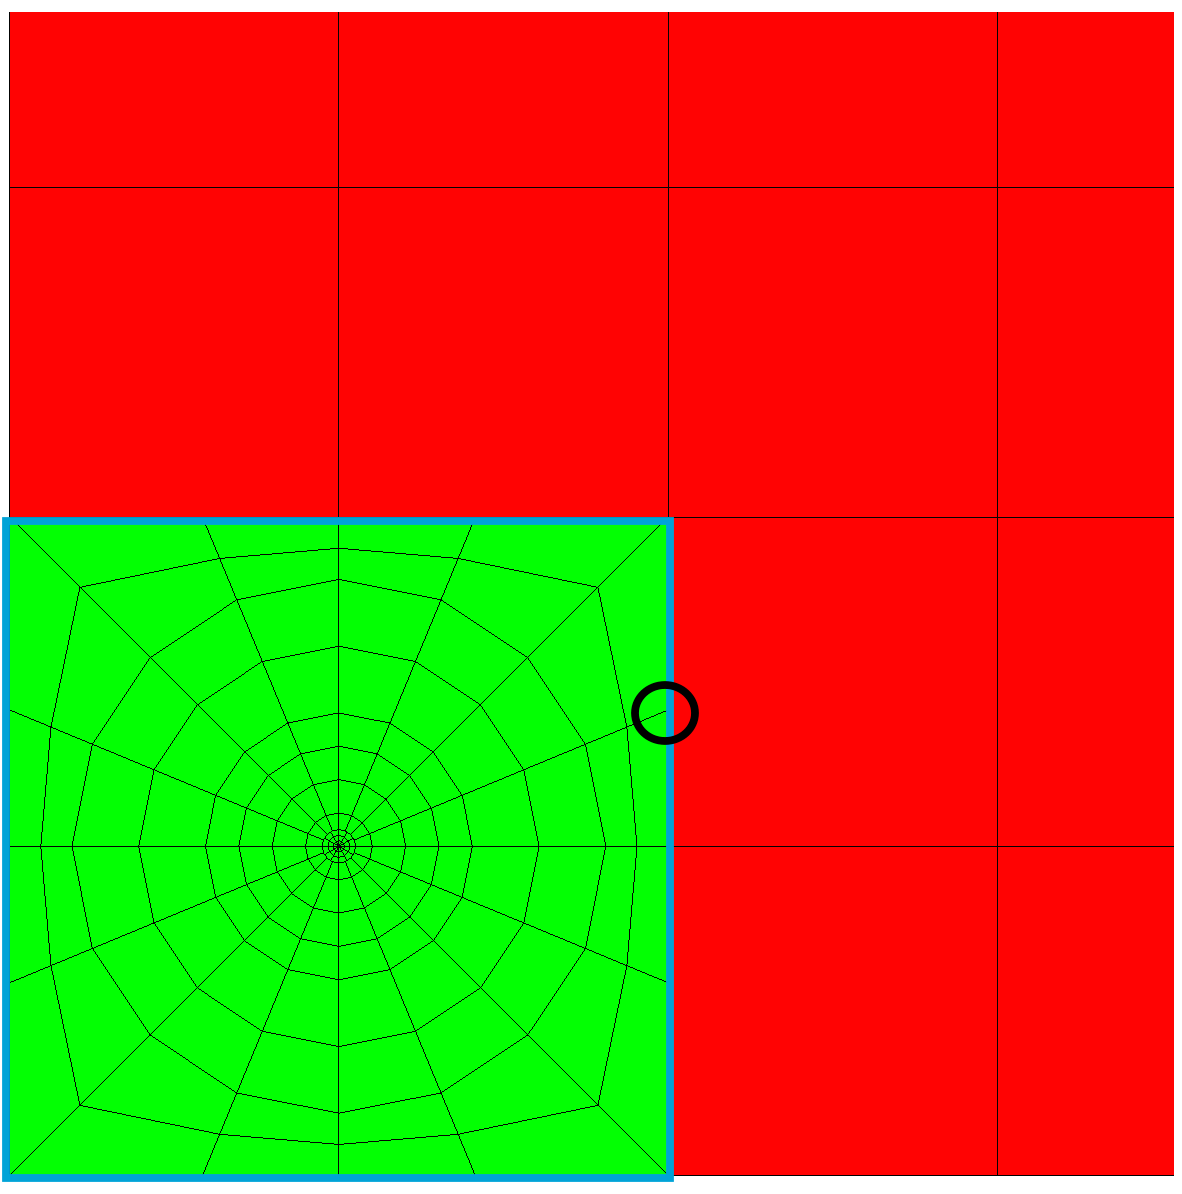
\includegraphics[scale=0.2]{../figures/hanging_node_spiderweb_example.png}
   \caption{A hanging node (circled in black) on a subset boundary (highlighted in blue).}
   \label{hanging_node}
\end{figure}

Both approaches to load balancing move cut lines in order to redistribute cells more evenly throughout subsets. We define a metric describing how imbalanced our problem is:
\begin{equation}
f =\frac{\underset{ijk}{\text{max}}(N_{ijk})}{\frac{N_{tot}}{I\cdot J\cdot K}},
\label{metric_def}
\end{equation}
where $f$ is the load balance metric, $N_{ijk}$ is the number of cells in subset $(i,j,k)$, $N_{tot}$ is the global number of cells in the problem, and $I$, $J$, and $K$ are the total number of subsets in the $x$, $y$, and $z$ directions, respectively. The metric is a measure of the maximum number of cells per subset divided by the average number of cells per subset. For a perfectly balanced problem, $f = 1$.

Figure~\ref{redistribute} illustrates an example of redistributing the cut planes in $x$ to balance the cells per column.
\begin{figure}[H]
\centering
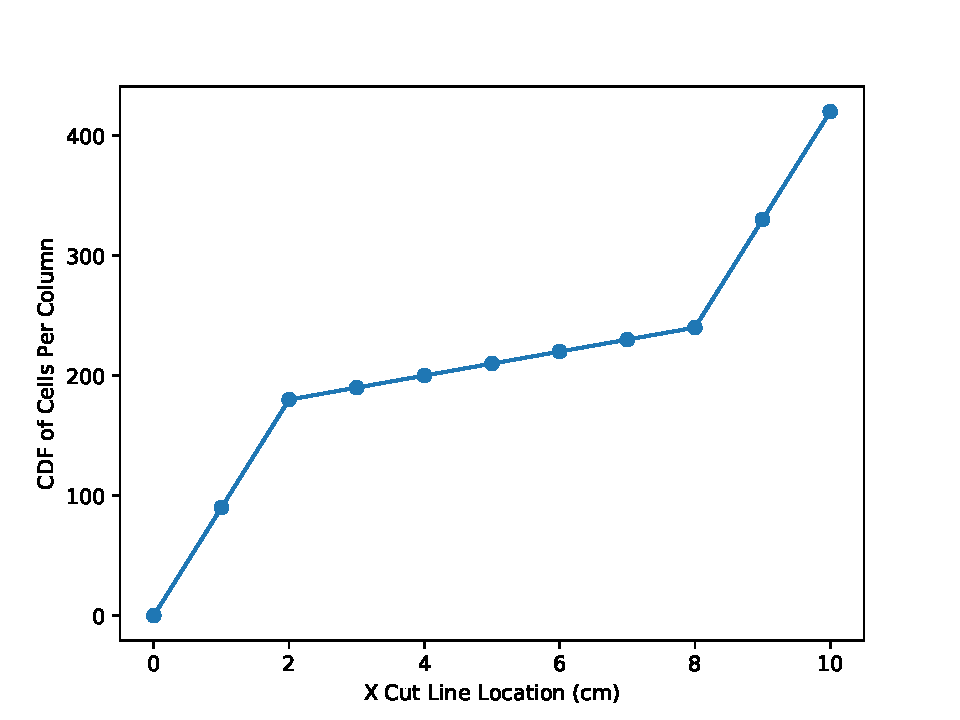
\includegraphics[scale=0.4]{../figures/spiderweb_redistribute_before_sparse.pdf}
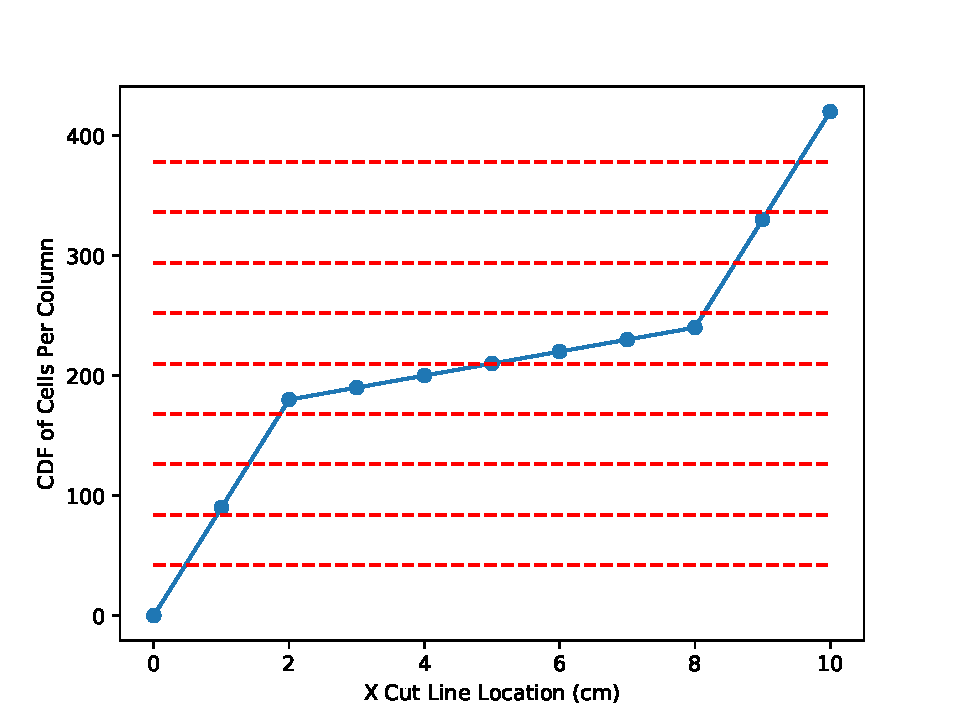
\includegraphics[scale=0.4]{../figures/spiderweb_redistribute_after_sparse.pdf}
\caption{The use of the CDF of cells per column to redistribute the cut lines in X.}
\label{redistribute}
\end{figure}
The image on the left side of Fig.~\ref{redistribute} shows the CDF of the cells per column in Fig.~\ref{partitioning_example}. The red lines on the right side of Fig.~\ref{redistribute} show the ideal equal number of cells per column. The x-value of the intersection of these red lines and the CDF are where the cut lines are redistributed to.

In order to decide the necessity of redistributing a dimension's cut lines/planes, we use dimensional sub-metrics of the following form:
\begin{equation}
f_{Z} = \frac{\underset{k}{\text{max}}[\sum_{i,j} N_{ijk}]}{\frac{N_{tot}}{K}},
\label{f_z}
\end{equation}
where $K$ is the total number of z-planes.
Equation \ref{f_z} is a metric defining how imbalanced the problem's planes are. It calculates the maximum cells per plane divided by the average cells per plane. If $f_K$ is greater than a predefined tolerance, the z cut planes are redistributed using the process in Fig.~\ref{redistribute}.

%%%%%%%%%%%%%%%%%%%%%%%%%%%%%%%%%%%%%%%%%%%%%%%%%%%%%%%%%%%%%%%%%%%%%%%%%%%%%%%%%%%
\subsection{Original Load-Balancing Algorithm}
\label{sec:og_lb}
%%%%%%%%%%%%%%%%%%%%%%%%%%%%%%%%%%%%%%%%%%%%%%%%%%%%%%%%%%%%%%%%%%%%%%%%%%%%%%%%%%%

The initial approach to load balancing was implemented on 2D extruded meshes, meaning the mesh is balanced in the 2D plane and then extruded, yielding a balanced 3D mesh. The metrics for this algorithm are defined as follows:
\begin{align}
f &= \frac{\underset{ij}{\text{max}}(N_{ij})}{\frac{N_{tot}}{I\cdot J}}  \label{og_metric}\\
f_X &= \frac{\underset{i}{\text{max}}[\sum_{j} N_{ij}] } {\frac{N_{tot}}{I}} \label{og_i_metric} \\
f_Y &= \frac{\underset{j}{\text{max}}[\sum_{i} N_{ij}] } {\frac{N_{tot}}{J}} \label{og_j_metric}
\end{align}
Equation \ref{og_metric} mirrors Eq. \ref{metric_def} for 2 dimensions, and Eqs. \ref{og_i_metric} and \ref{og_j_metric} define the column and row-wise metrics respectively.

 Algorithm \ref{initial_algorithm} summarizes the original approach to load balancing meshes in PDT.
\begin{algorithm}[H]
\caption{The original load-balancing algorithm.}
\label{initial_algorithm}
\begin{algorithmic}

\WHILE{$f > 1 + \text{tol}_{\text{subset}}$}
  \IF {$f_X > 1 + \text{tol}_{\text{col}}$}
    \STATE Redistribute the X cut lines.
  \ENDIF
  \IF {$f_Y > 1 + \text{tol}_{\text{row}}$}
  	\STATE Redistribute the Y cut lines.
  \ENDIF
\ENDWHILE
\end{algorithmic}
\end{algorithm}
While the problem is not balanced:
\begin{itemize}
  \item Check if the columns are balanced, and if not redistribute the X cut lines.
  \item Check if the rows are balanced, and if not redistribute the Y cut lines.
  \item Repeat until the mesh is balanced or until a maximum number of iterations is reached.
\end{itemize}

The original load-balancing algorithm placed cut lines in all dimensions all the way through the mesh.
This created an orthogonal partitioning where each subset had an equivalent number of neighbors, which was done to preserve the provably optimal sweep partitioning described by Adams et. al \cite{mpadams2013,mpadams2015,mpadamsjcp}.
However, there are theoretical limits to load balancing in this fashion. Figure~\ref{2dgeneral} shows a simple 2D subset layout with $M$ unaligned patches with $N$ cells each.

\begin{figure}[H]
\centering
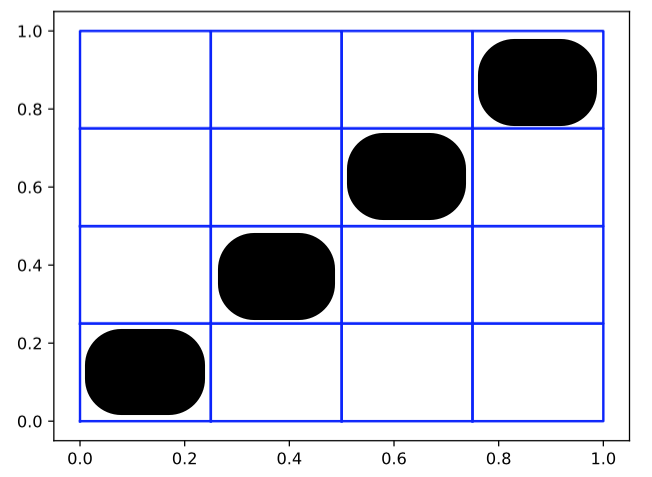
\includegraphics[scale=0.4]{../figures/theoretical_plot.png}
 \caption{A 2D subset layout with $M$ unaligned patches of high mesh density $N$.}
\label{2dgeneral}
\end{figure}
The subset layout is $M^2$, but only $M$ subset have significant work, leading to a theoretical limit for the load imbalance factor:
\begin{equation}
f= \frac{N}{(MN+C)/M^2} \xrightarrow{N\to \infty} \frac{N}{N/M} = M.
\end{equation}
Due to this theoretical limit, the load-balancing-by-dimension algorithm was developed.

%%%%%%%%%%%%%%%%%%%%%%%%%%%%%%%%%%%%%%%%%%%%%%%%%%%%%%%%%%%%%%%%%%%%%%%%%%%%%%%%%%%
\subsection{Load-Balancing-by-Dimension Algorithm}
\label{sec:lbd}
%%%%%%%%%%%%%%%%%%%%%%%%%%%%%%%%%%%%%%%%%%%%%%%%%%%%%%%%%%%%%%%%%%%%%%%%%%%%%%%%%%%

The load-balancing-by-dimension by dimension (LBD) algorithm, similar to the original load-balancing algorithm, relies on the movement of cut lines/planes to redistribute mesh cells in a more balanced manner.
However, cut lines are no longer required to go all the way through the mesh, and the load-balancing-by-dimension algorithm is fully extensible to 3 dimensions.
The load-balancing-by-dimension algorithm is summarized by:
\begin{enumerate}
  \item Slice the mesh in $z$ and redistribute cut planes until each plane has approximately an equivalent number of cells.
  \item For each $z$ layer, slice the layer in columns and redistribute the $x$ cut lines until each column has an approximately equivalent number of cells.
  \item For each column within each $z$ layer, slice the column in rows and redistribute the $y$ cut lines until each row has an approximately equivalent number of cells.
\end{enumerate}

We once again use dimensional sub-metrics to determine whether or not a dimension's cut lines/planes need to be redistributed. The $z$ dimension's sub-metric is defined by Eq. \ref{f_z}. For the LBD algorithm, there are $K$ column-wise metrics, one for each $z$ layer:
\begin{equation}
f_{X,k} = \frac{ \underset{i}{\text{max}}[ \sum_{j} N_{ijk}]  }  {\frac{N_{tot,k}}{I}},
\label{lbd_x_metric}
\end{equation}
where $N_{tot,k}$ is the number of cells in layer $k$.
Equation \ref{lbd_x_metric} defines the column-wise metric for layer $k$, or the maximum number of cells per column in layer $k$ divided by the average number of cells per column in layer $k$.

For the LBD algorithm, there are $K\cdot I$ row-wise metrics, one for each column in each $z$ layer:
\begin{equation}
f_{Y,k,i} = \frac{\underset{j}{\text{max}} N_{ijk} } {\frac{N_{tot,k,i}}{J}},
\label{lbd_y_metric}
\end{equation}
where $N_{tot,k,i}$ is the number of cells in column $i$ in layer $k$.
Equation \ref{lbd_y_metric} defines the row-wise metric for layer $k$ in column $i$, or the maximum number of cells per row in column $i$ in layer $k$ divided by the average number of cells per row in column $i$ in layer $k$.

Algorithm \ref{lbd} details the load-balancing-by-dimension algorithm.
\begin{algorithm}[H]
\caption{The load-balancing-by-dimension algorithm.}
\label{lbd}
\begin{algorithmic}

  \WHILE {$f_{Z} > 1 + \text{tol}_{\text{K}}$}
    \STATE Redistribute the Z cut planes.
  \ENDWHILE

  \FOR {$k$ in $K$}
    \WHILE {$f_{X,k} > 1 + \text{tol}_{\text{I}}$}
      \STATE Redistribute the X cut lines within layer $k$.
    \ENDWHILE
  \ENDFOR

  \FOR{$k$ in $K$}
    \FOR{$i$ in $I$}
      \WHILE {$f_{Y,k,i} > 1 +  \text{tol}_{\text{J}}$ }
        \STATE Redistribute the Y cut lines in column $i$ in layer $k$.
      \ENDWHILE
    \ENDFOR
  \ENDFOR

  \STATE Calculate $f$.
\end{algorithmic}
\end{algorithm}

Figure~\ref{alg_illustration} illustrates the behavior of both algorithms after 5 iterations. In Fig.~\ref{3x3_lb}, we see the partitions cutting across the entire domain, with the $x$ and $y$ cut lines moving into the denser geometric features in the corners to more evenly distribute cells. In Fig.~\ref{3x3_lbd}, we see the $x$ partitions cutting across the entire domain, but the $y$ partitions being redistributed by column. The $y$ partitions are moved into the respective geometric features in the appropriate columns in order to better balance the problem.

\begin{figure}[H]
\centering
\begin{subfigure}[t]{\textwidth}
\centering
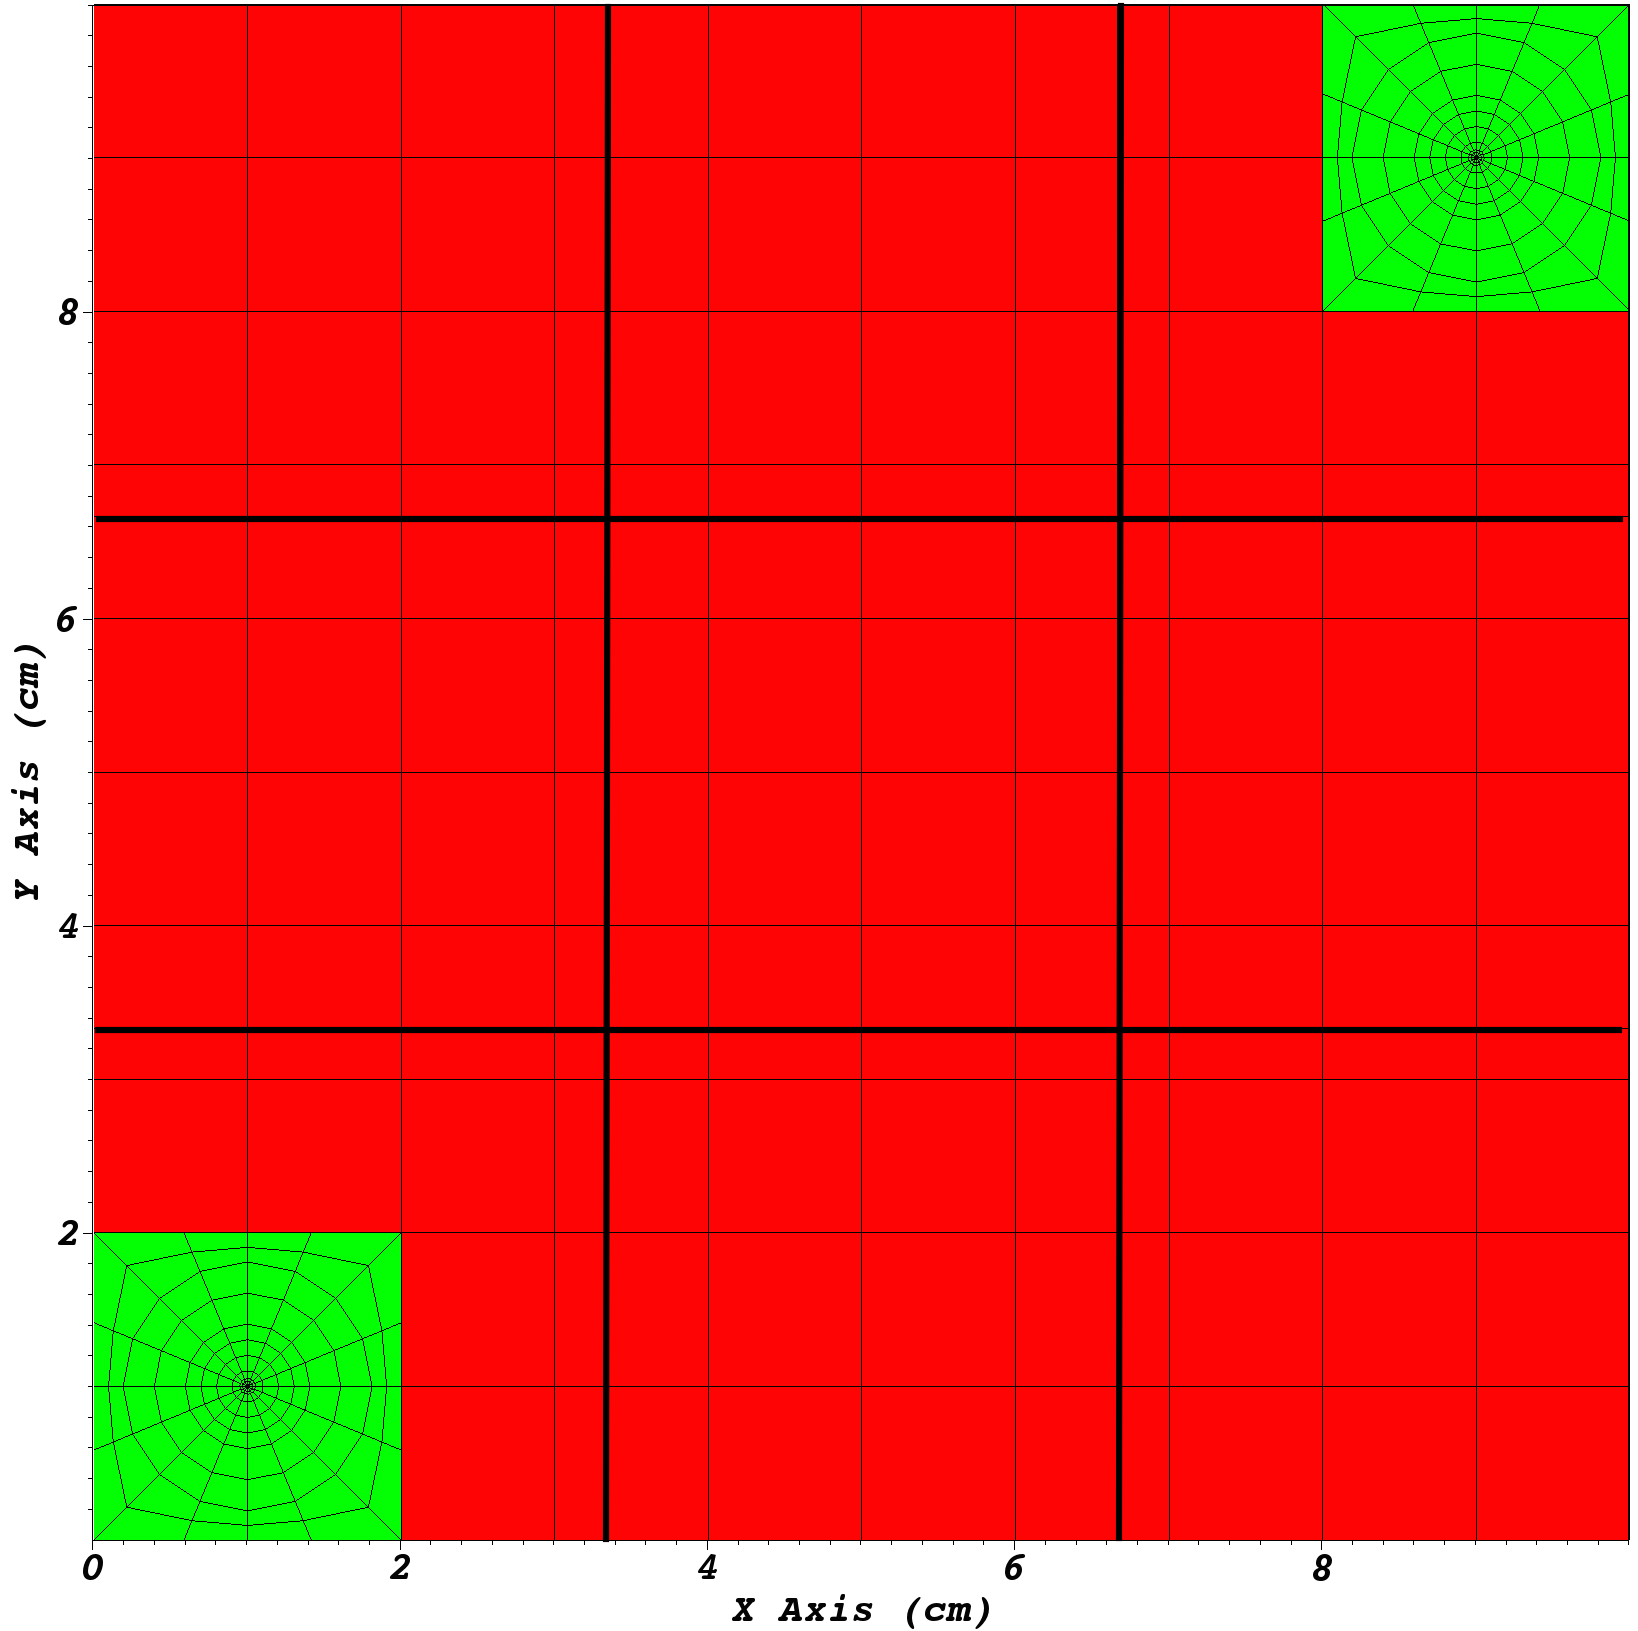
\includegraphics[scale=0.15]{../figures/ubp_3x3_regular.png}
\caption{No load balancing, $f = 3.41$.}
\label{3x3_regular}
\end{subfigure}
\begin{subfigure}[b]{0.49\textwidth}
\centering
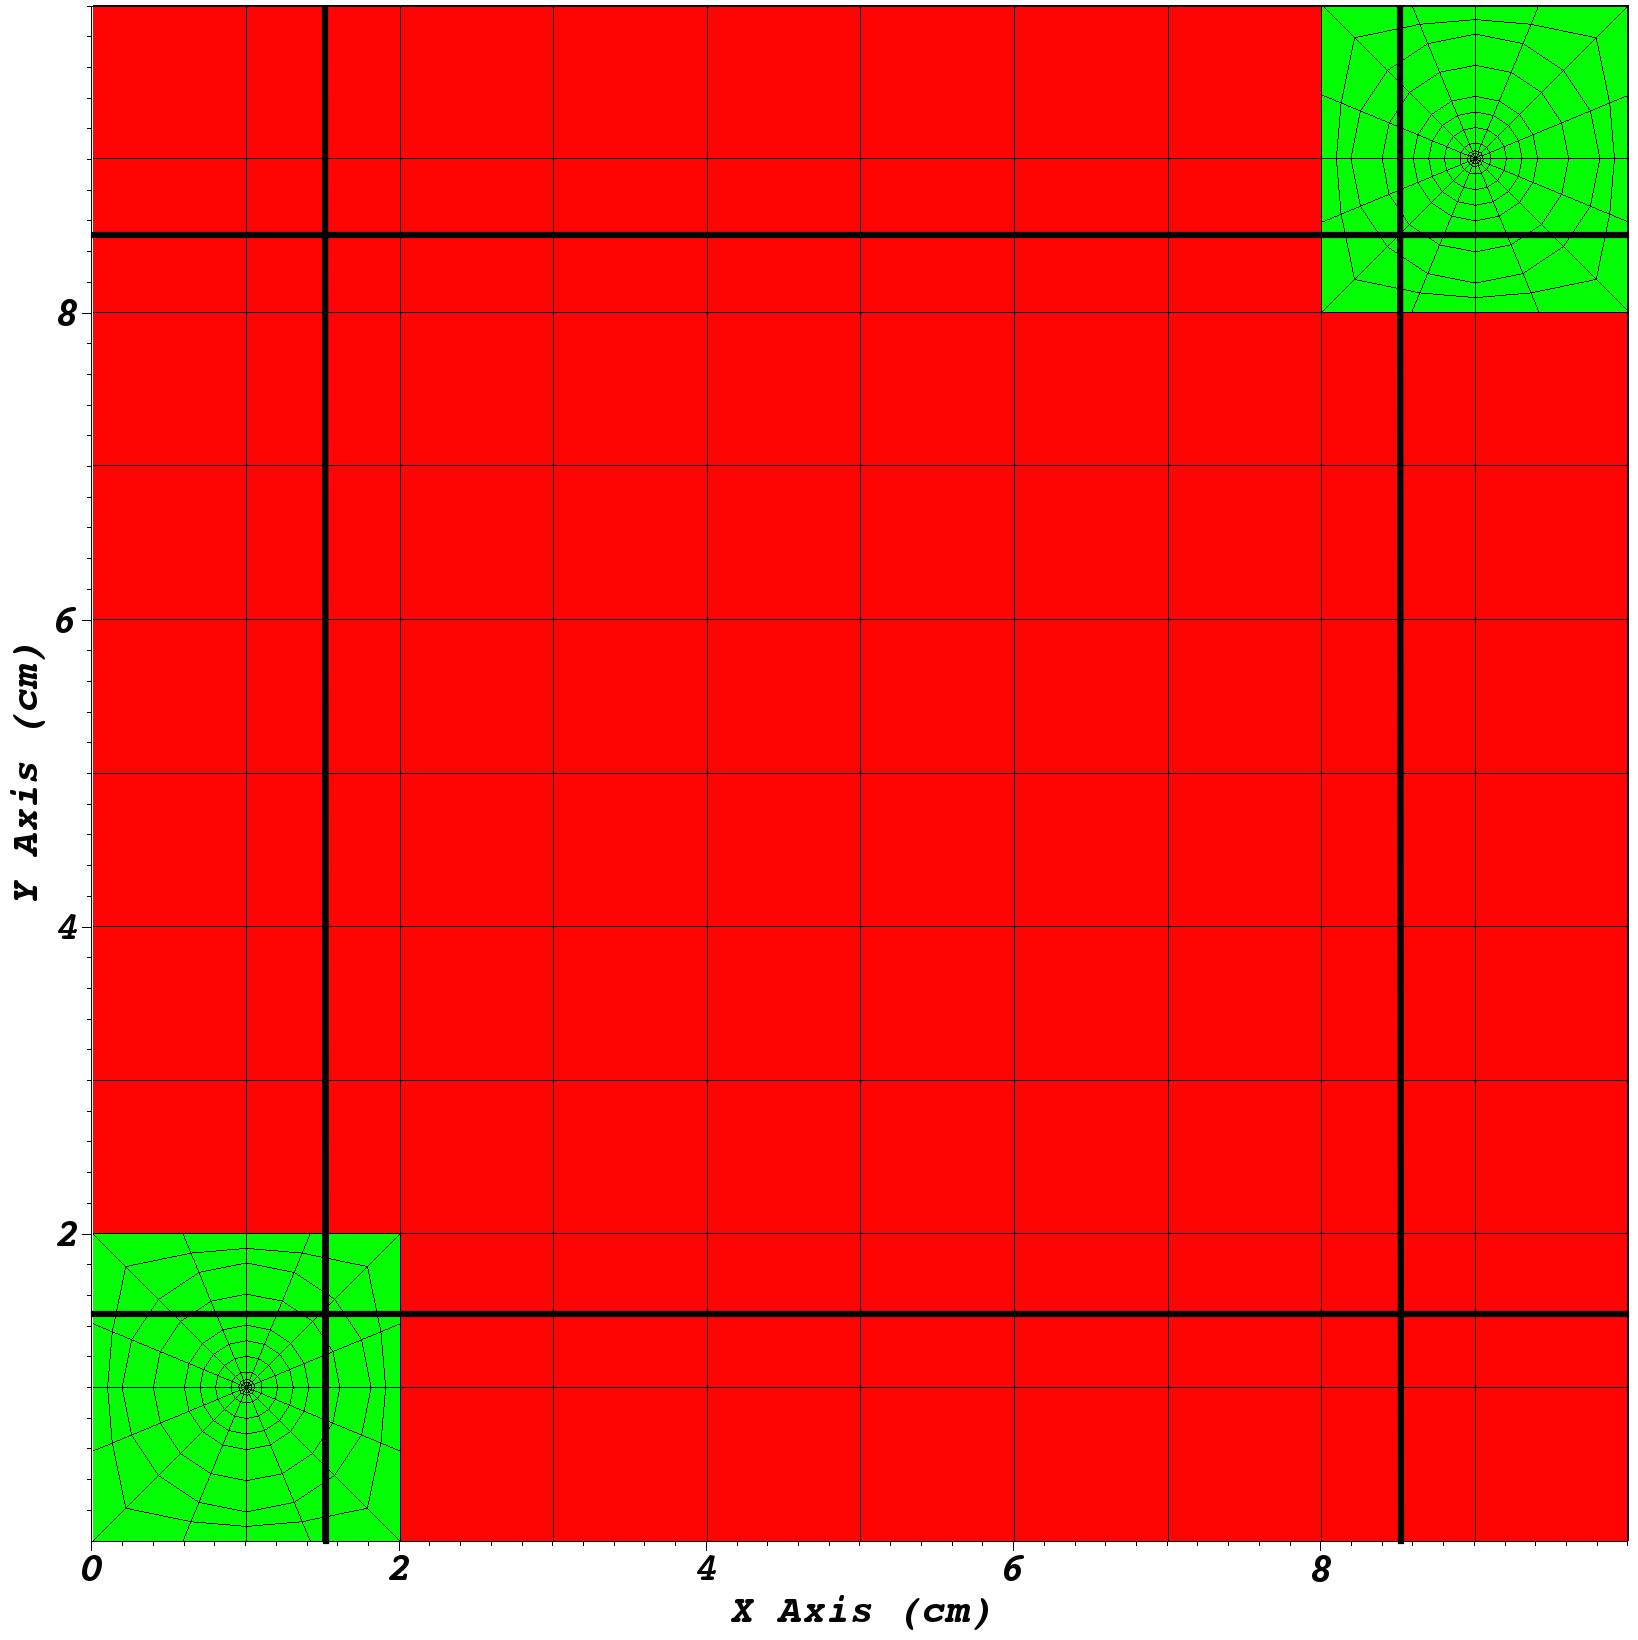
\includegraphics[scale=0.13]{../figures/ubp_3x3_lb.png}
\caption{5 load balancing iterations, $f = 2.58$.}
\label{3x3_lb}
\end{subfigure}
\begin{subfigure}[b]{0.49\textwidth}
\centering
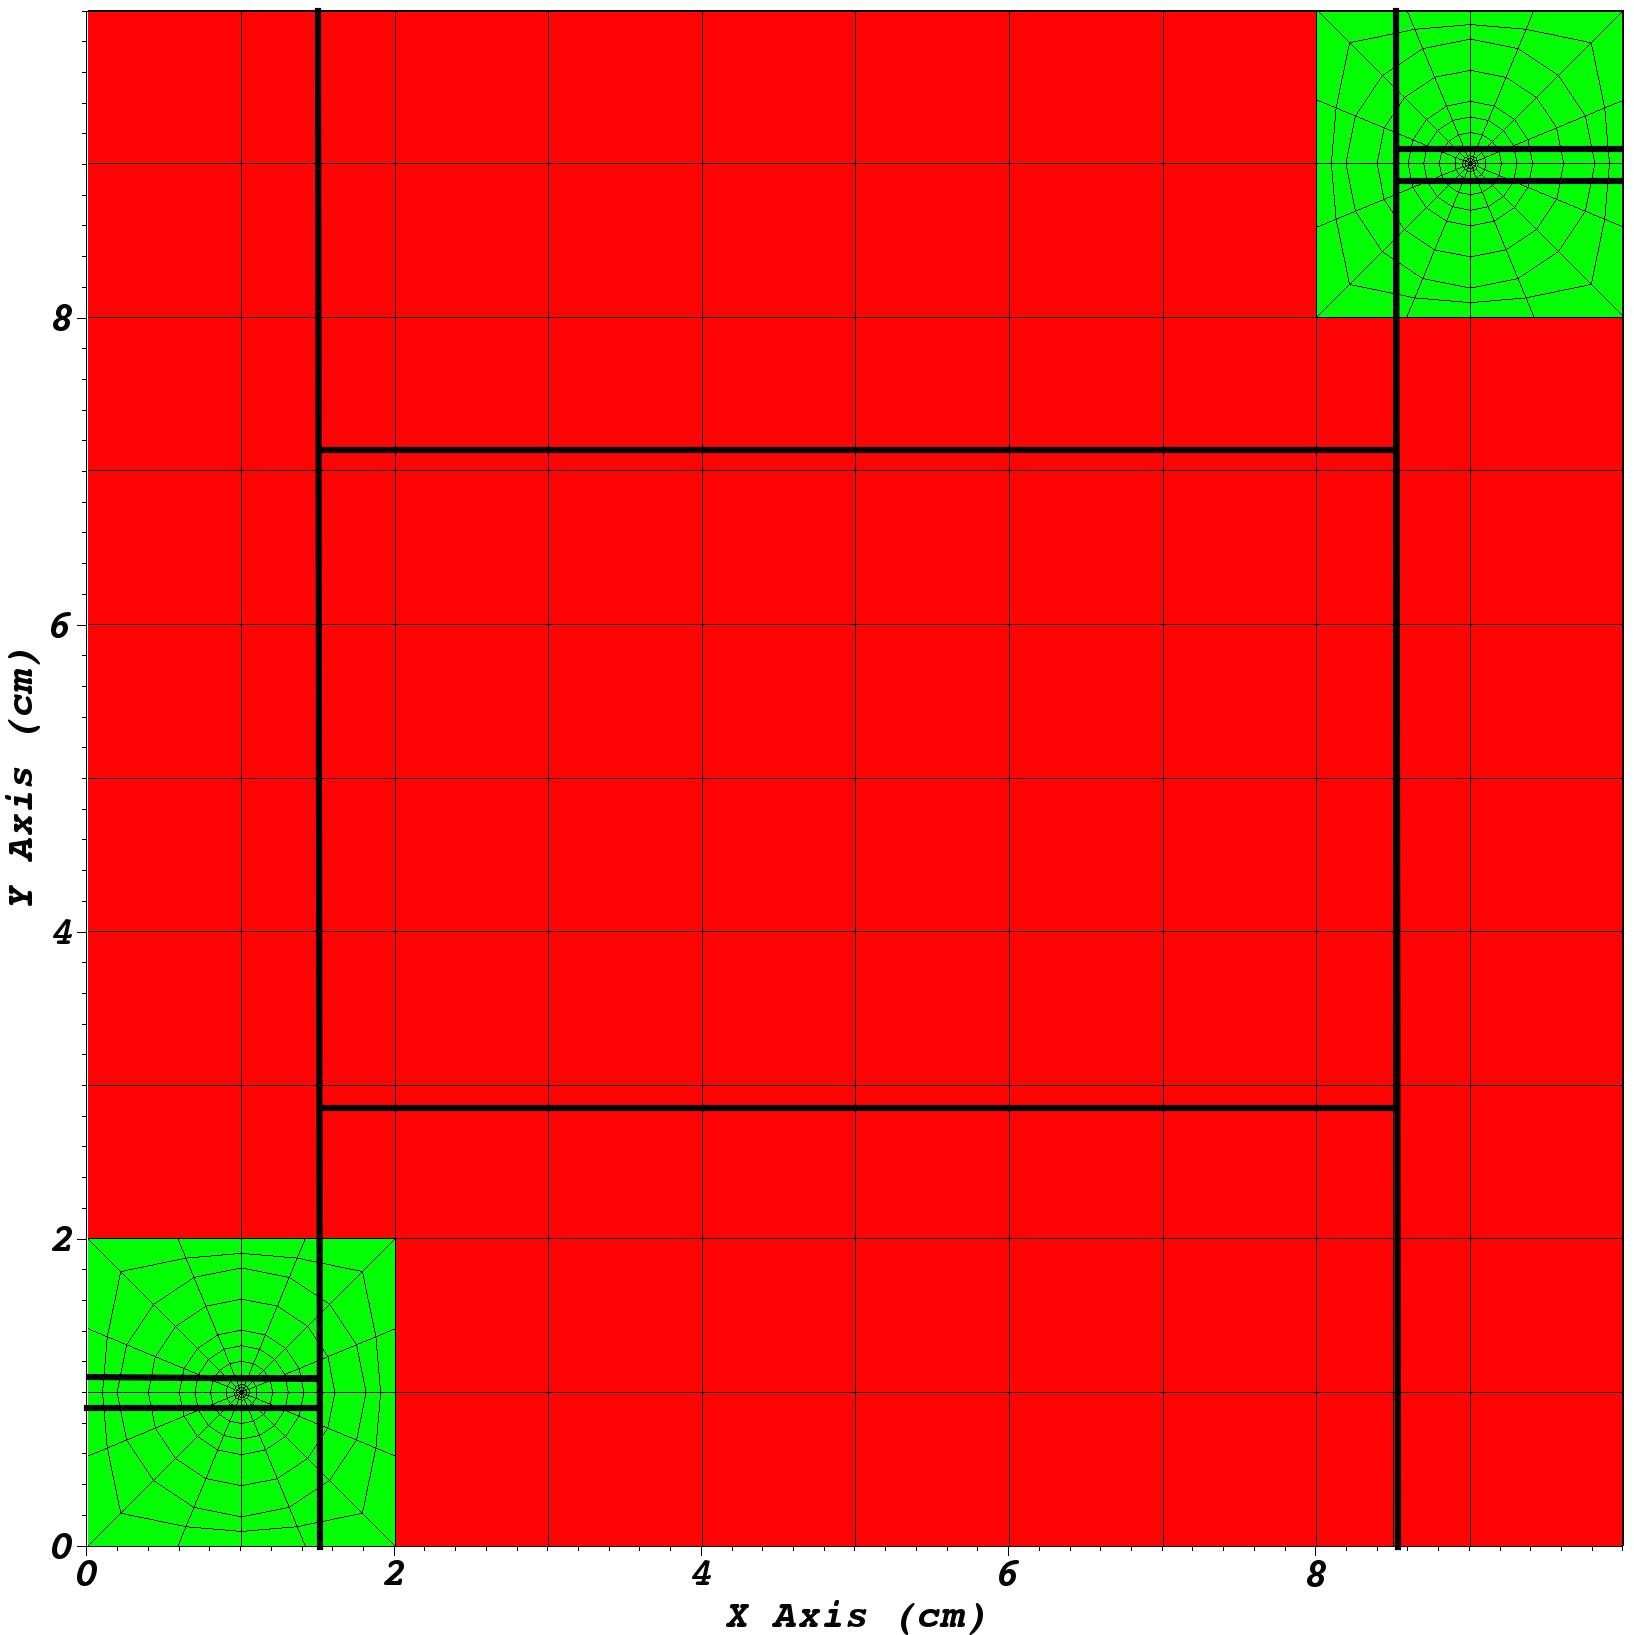
\includegraphics[scale=0.13]{../figures/ubp_3x3_lbd.png}
\caption{5 load-balancing-by-dimension iterations, $f = 1.49$.}
\label{3x3_lbd}
\end{subfigure}
\caption{A demonstration of the original load balancing and load-balancing-by-dimension algorithms on an unstructured mesh partitioned into 3x3 subsets.}
\label{alg_illustration}
\end{figure}

%%%%%%%%%%%%%%%%%%%%%%%%%%%%%%%%%%%%%%%%%%%%%%%%%%%%%%%%%%%%%%%%%%%%%%%%%%%%%%%%%%%
\subsection{Parametric Study of the Original Load Balancing and the Load-Balancing-by-Dimension Algorithms}
%%%%%%%%%%%%%%%%%%%%%%%%%%%%%%%%%%%%%%%%%%%%%%%%%%%%%%%%%%%%%%%%%%%%%%%%%%%%%%%%%%%
To study the behavior and effectiveness of both the original load balancing and the load-balancing-by-dimension algorithm, a parametric study was run on the mesh shown in Fig.~\ref{partitioning_example}.
This mesh was chosen because it is inherently imbalanced as there are two dense geometric features in opposing corners with a sparse region in between.

%%%%%%%%%%%%%%%%%%%%%%%%%%%%%%%%%%%%%%%%%%%%%%%%%%%%%%%%%%%%%%%%%%%%%%%%%%%%%%%%%%%
\subsubsection{Parametric study on the unbalanced pin mesh}
%%%%%%%%%%%%%%%%%%%%%%%%%%%%%%%%%%%%%%%%%%%%%%%%%%%%%%%%%%%%%%%%%%%%%%%%%%%%%%%%%%%

The study calculates $f$ for the mesh with no load balancing iterations, 5 original load balancing iterations, and 5 load-balancing-by-dimension iterations.
The mesh is partitioned into 2 to 10 subsets in each dimension for all load balancing formats.
Figure~\ref{metric_study} shows the results of this parametric study.
The results are tabulated in Table \ref{metric_study_table}.

With regular cut lines going through the mesh, $f_\text{reg}$ generally increases as the number of subsets increases.
As the number of cut lines increases, the number of cells added may also increase, driving up the maximum number of cells in each subset. It is important to note that in Eq. \ref{metric_def}, the average number of cells per subset used to calculate $f$ is the average number of cells per subset \textit{before} slicing through the mesh.
With more cut lines, the maximum number of cells per subset will increase while the average number of cells per subset will decrease, leading to an increase in $f$. There can be exceptions to this trend, as seen by ${f_\text{reg}}$ for 8 and 10 subsets in each dimension.
The cut lines with 10 subsets in each dimension lie on natural boundaries when evenly distributed.
A natural boundary is a mesh boundary that coincides with a subset boundary, adding no cells to the mesh.
Because no cells are added in the 10x10 case, $f_{\text{reg}}$ with 10 subsets in each dimension is lower than $f_{\text{reg}}$ with 8 subsets in each dimension.

For the load balanced and load-balanced-by-dimension cases, we see a similar increasing trend for $f$, although it is not quite as consistent for the load-balanced-by-dimension cases.
\begin{figure}[H]
\centering
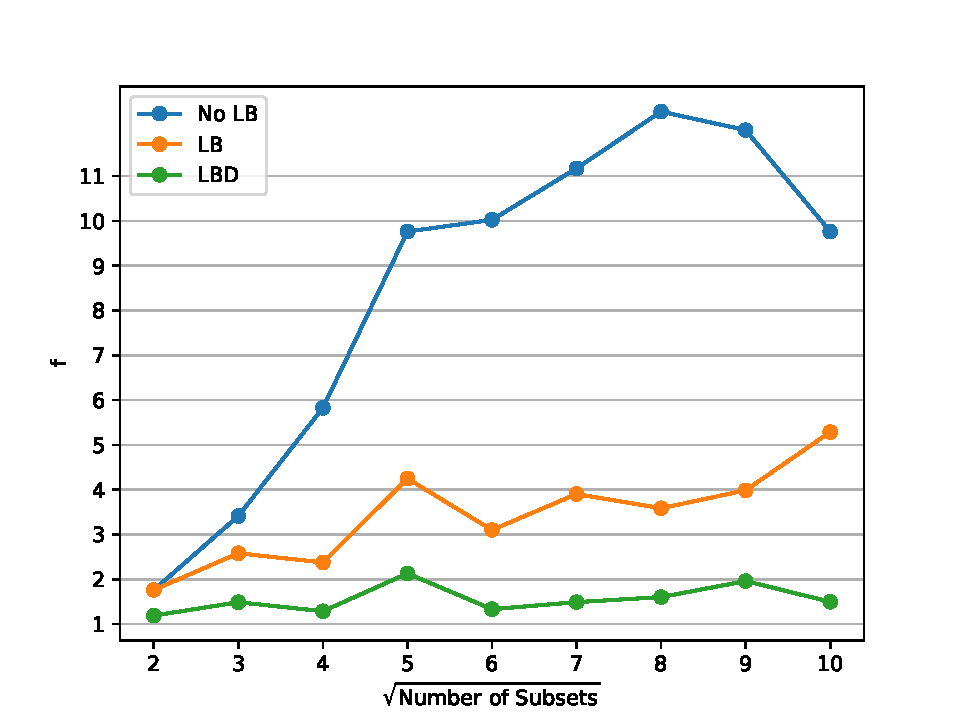
\includegraphics[scale=0.7]{../figures/metric_study.pdf}
\caption{The results of the parametric study with no load balancing, 5 original load balancing iterations, and 5 load-balancing-by-dimension iterations.}
\label{metric_study}
\end{figure}
\begin{table}[H]
\centering
\caption{The tabulated results of the parametric study shown in Fig.~\ref{metric_study} with no load balancing, 5 original load balancing iterations (LB), and 5 load-balancing-by-dimension (LBD) iterations.}
\label{metric_study_table}
\scalebox{0.8}{
\begin{tabular}{c|c|c|c}
\textbf{$\sqrt{\text{Num Subsets}}$} & \bf $f_{\text{reg}}$ & \bf $f_{\text{LB}}$  & \bf $f_{\text{LBD}}$\\ \hline
2&1.76&1.76&1.19\\ \hline
3&3.41&2.58&1.49\\ \hline
4&5.83&2.38&1.29\\ \hline
5&9.76&4.25&2.13\\ \hline
6&10.02&3.1&1.33\\ \hline
7&11.17&3.9&1.49\\ \hline
8&12.44&3.59&1.6\\ \hline
9&12.03&3.99&1.96\\ \hline
10&9.76&5.29&1.5
\end{tabular}}
\end{table}

Table \ref{metric_improvement} shows the percent decrease in $f$ with the original load balancing algorithm and the load-balancing-by-dimension algorithm relative to no load balancing, and the percent decrease in $f$ with the load-balancing-by-dimension algorithm relative to the original load balancing algorithm.
There is consistent improvement for both algorithms for all cases, and the improvement both load balancing algorithms relative to no algorithm generally increases as the number of subsets increases. The improvement of load-balancing-by-dimension over load balancing is notable, with a minimum improvement of 32.43\% and a maximum improvement of 71.66\%.
\begin{table}[H]
\centering
\caption{The percent decrease of $f$ with the original load balancing algorithm (LB) and the load-balancing-by-dimension algorithm (LBD) relative to no load balancing, and the percent decrease of $f$ with the load-balancing-by-dimension algorithm relative to the original load balancing algorithm.}
\label{metric_improvement}
\begin{tabular}{c|c|c|c}
\centering
\textbf{$\sqrt{\text{Num Subsets}}$} & \textbf{LB v. No LB}  & \textbf{LBD v. No LB} & \textbf{LBD v. LB} \\ \hline
2&0.0\%&32.43\%&32.43\%\\ \hline
3&24.38\%&56.38\%&42.33\%\\ \hline
4&59.21\%&77.9\%&45.82\%\\ \hline
5&56.48\%&78.17\%&49.83\%\\ \hline
6&69.05\%&86.7\%&57.01\%\\ \hline
7&65.06\%&86.66\%&61.83\%\\ \hline
8&71.17\%&87.1\%&55.27\%\\ \hline
9&66.84\%&83.69\%&50.81\%\\ \hline
10&45.85\%&84.65\%&71.66\%
\end{tabular}
\end{table}

\FloatBarrier
%%%%%%%%%%%%%%%%%%%%%%%%%%%%%%%%%%%%%%%%%%%%%%%%%%%%%%%%%%%%%%%%%%%%%%%%%%%%%%%%%%%
\subsubsection{Parametric study on the Level-2 experiment mesh}
%%%%%%%%%%%%%%%%%%%%%%%%%%%%%%%%%%%%%%%%%%%%%%%%%%%%%%%%%%%%%%%%%%%%%%%%%%%%%%%%%%%

The same parametric study was run on an experiment that PDT simulates, the Level-2 experiment, shown in Fig.~\ref{level2_nocut_lbchapter}.
\begin{figure}[ht]
\centering
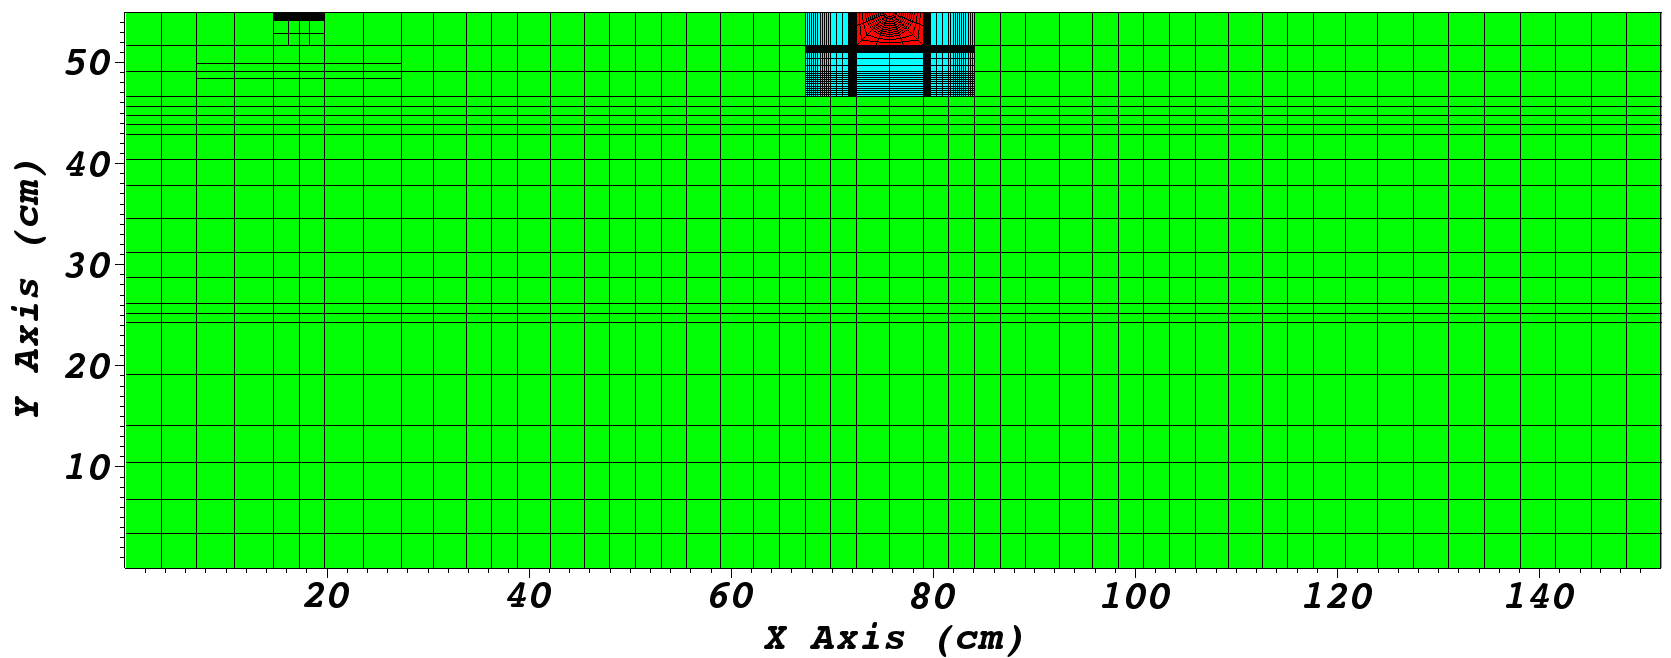
\includegraphics[scale=0.25]{../figures/level2_nocut.png}
\caption{The mesh for the Level-2 experiment.}
\label{level2_nocut_lbchapter}
\end{figure}
The Level-2 mesh contains a relatively uniform geometry throughout the mesh with one denser feature in the middle of the top boundary.
Fig.~\ref{level2_alg_illustration} shows the dense region of the Level-2 mesh with 7 regular, load-balanced, and load-balanced-by-dimension cuts.
%zoomed in photos
\begin{figure}[ht]
\centering
\begin{subfigure}[t]{\textwidth}
\centering
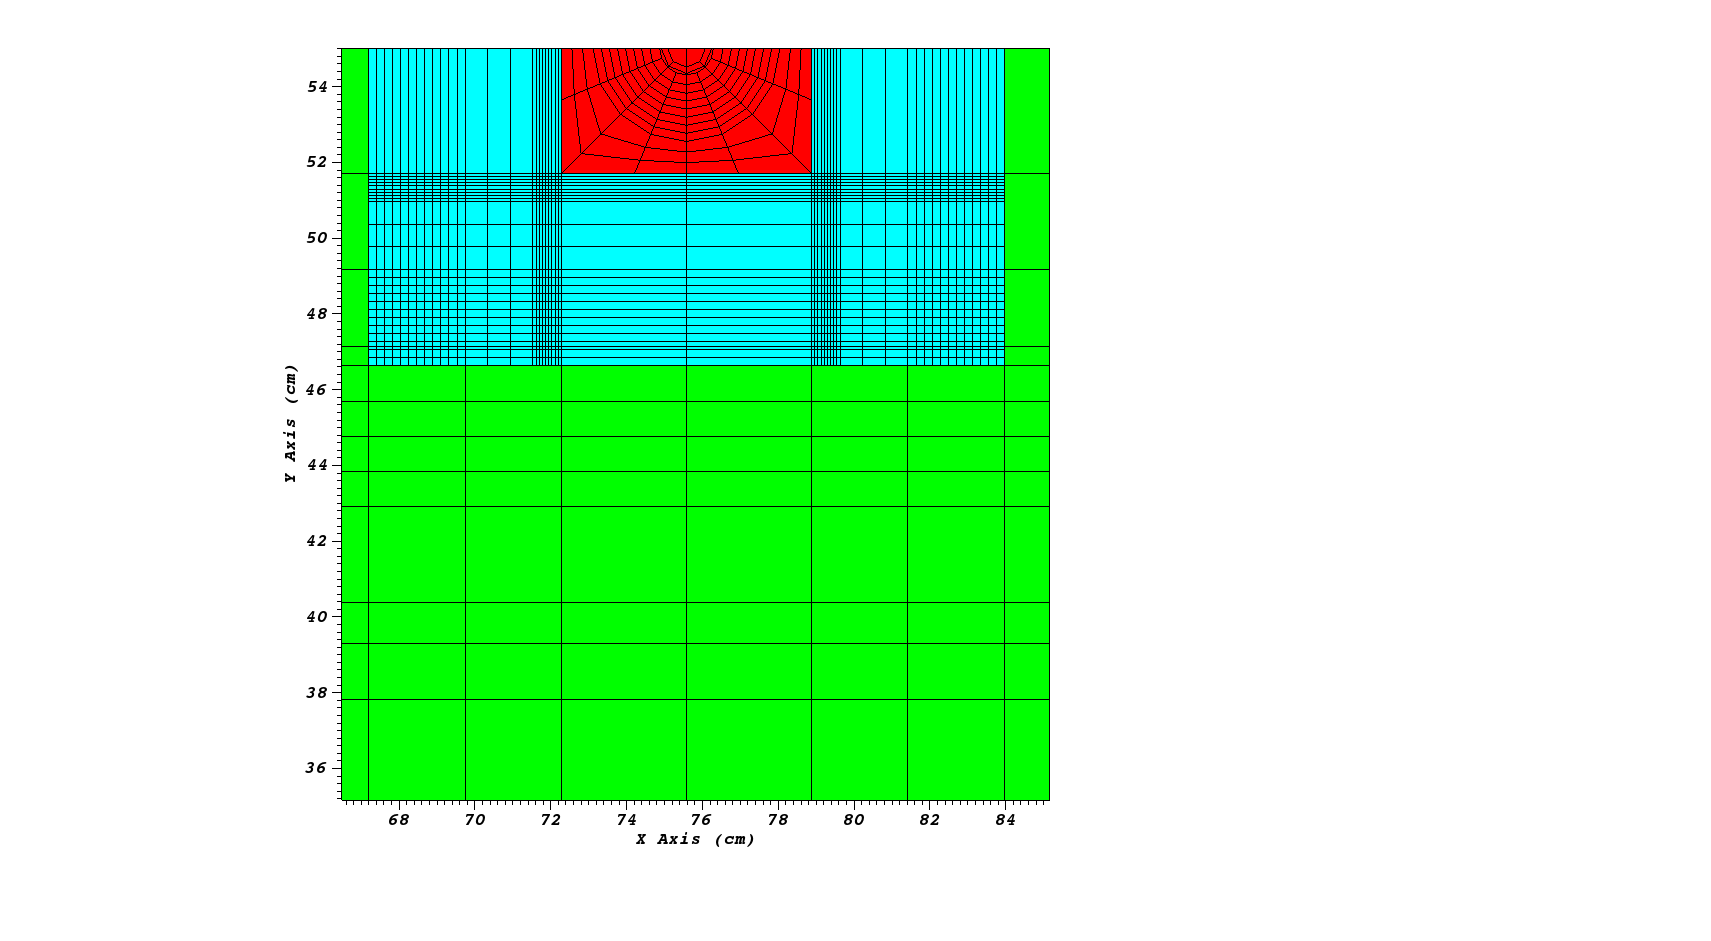
\includegraphics[scale=0.3]{../figures/level2_7_reg_zoom.png}
\caption{No load balancing.}
\label{7_regular}
\end{subfigure}
\begin{subfigure}[b]{\textwidth}
\centering
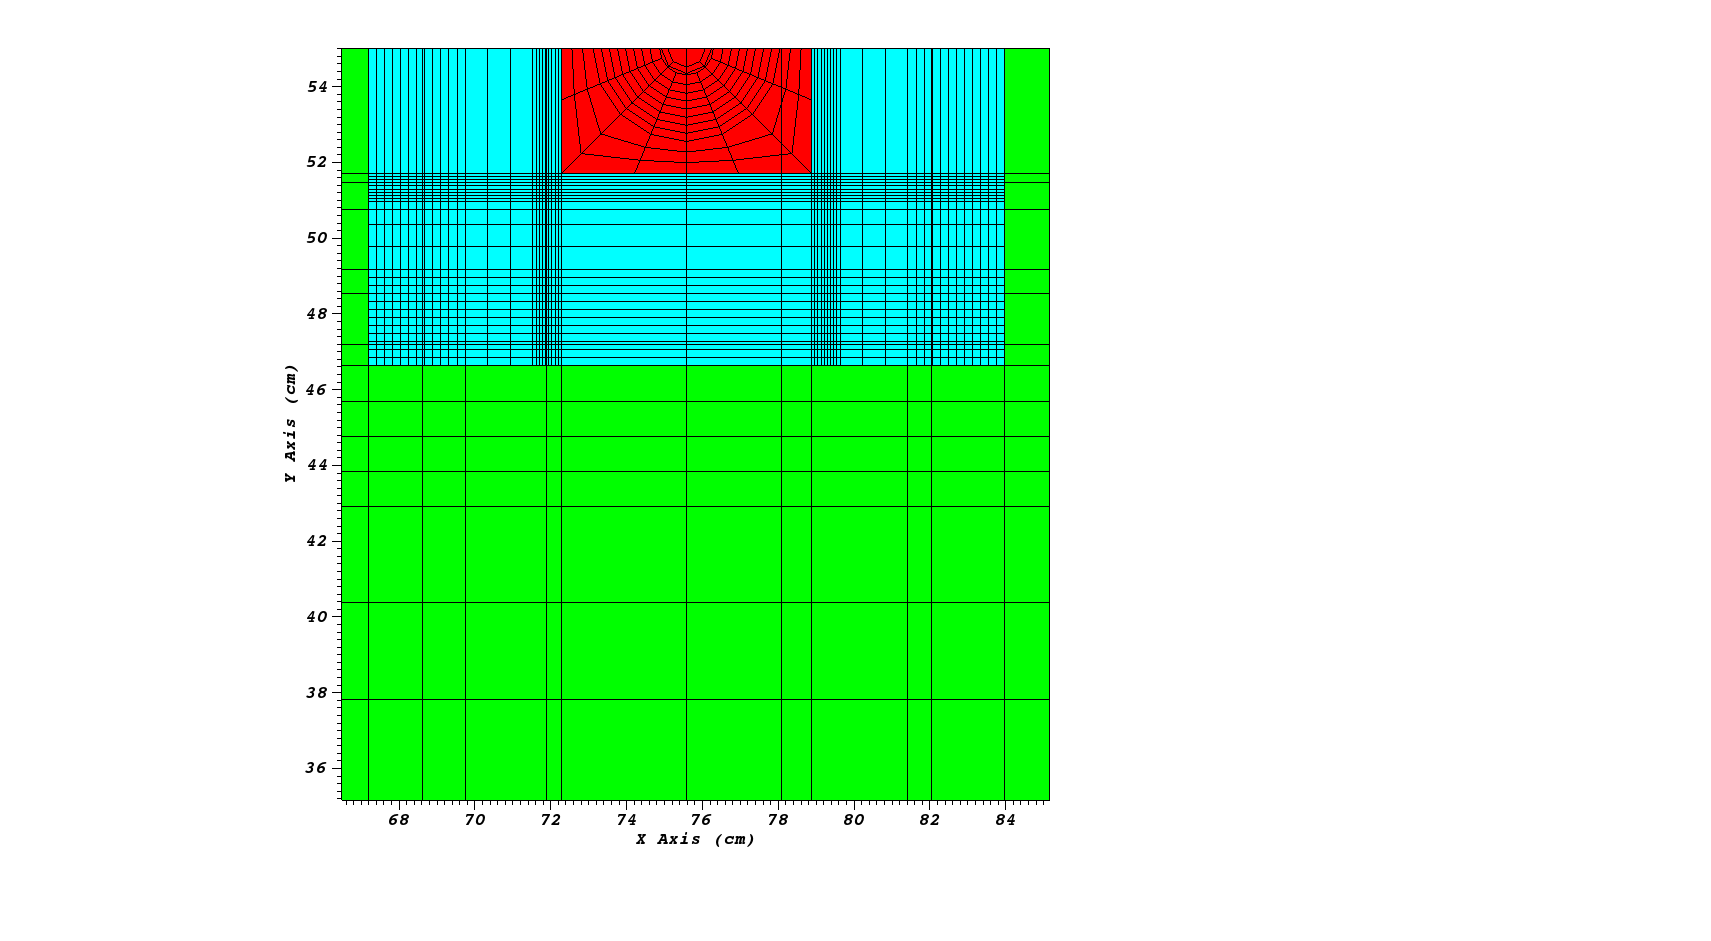
\includegraphics[scale=0.3]{../figures/level2_7_lb_zoom.png}
\caption{5 load balancing iterations.}
\label{7_lb}
\end{subfigure}
\begin{subfigure}[b]{\textwidth}
\centering
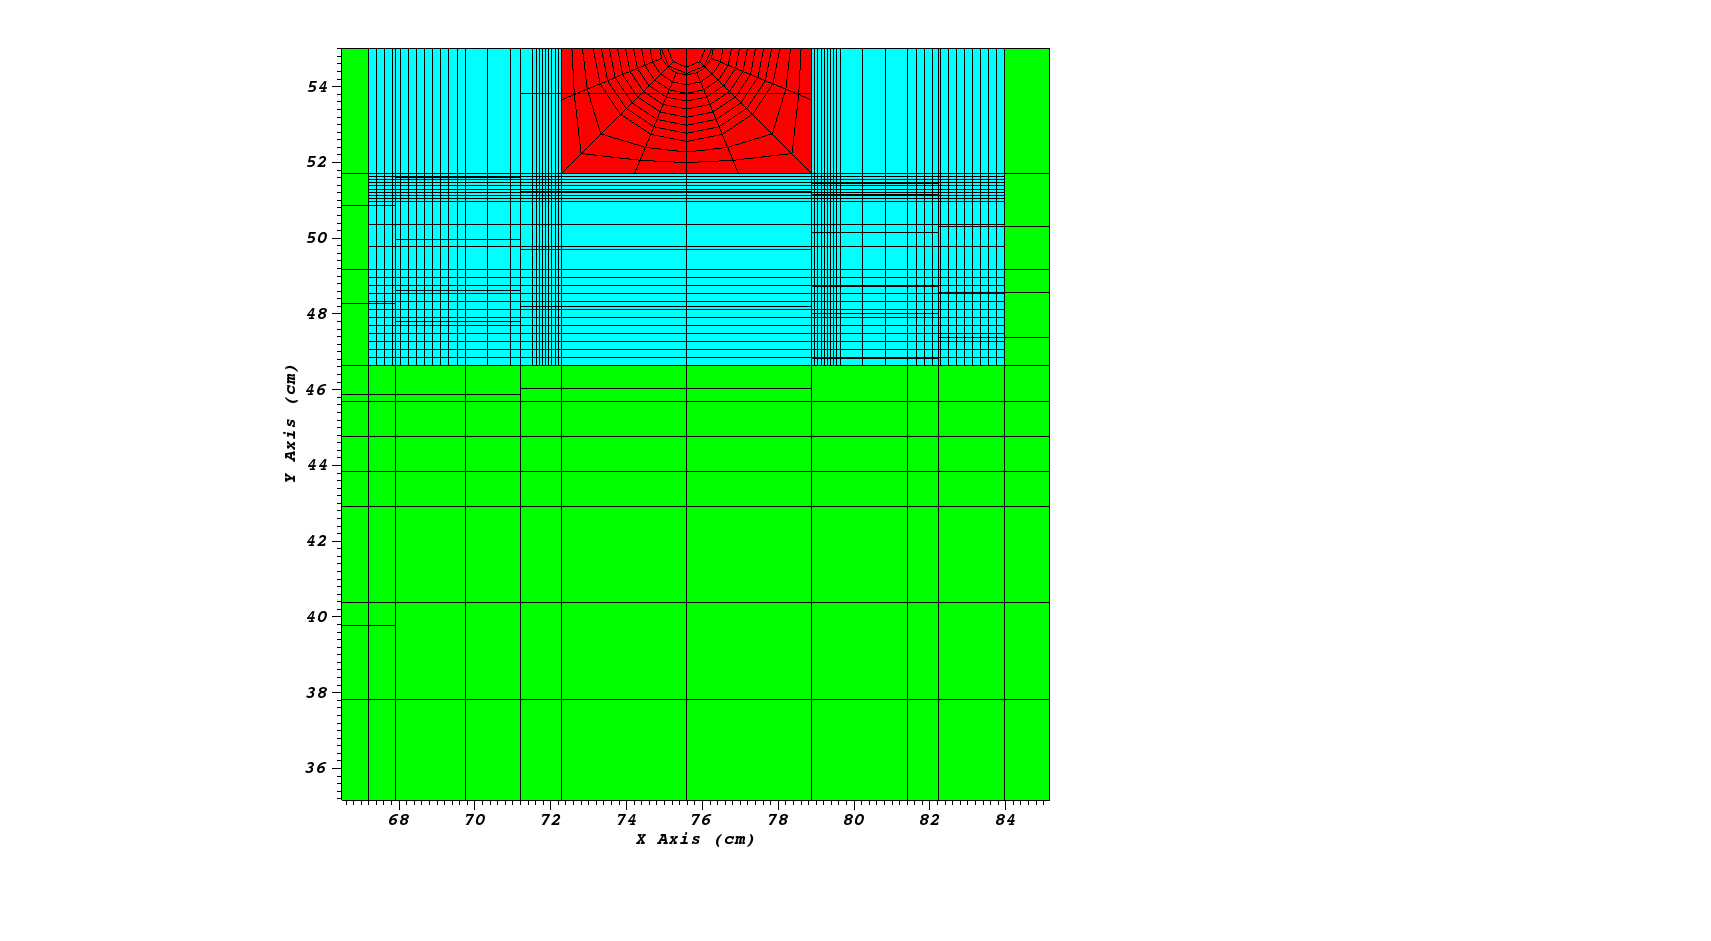
\includegraphics[scale=0.3]{../figures/level2_7_lbd_zoom.png}
\caption{5 load-balancing-by-dimension iterations.}
\label{7_lbd}
\end{subfigure}
\caption{A demonstration of the original load balancing and load-balancing-by-dimension algorithms on the Level-2 mesh partitioned into 7x7 subsets.}
\label{level2_alg_illustration}
\end{figure}
Figure~\ref{level2_metric_study} shows the results of this parametric study, which are tabulated in Table \ref{level2_metric_study_table}.
%%%%%%%
\begin{figure}[H]
\centering
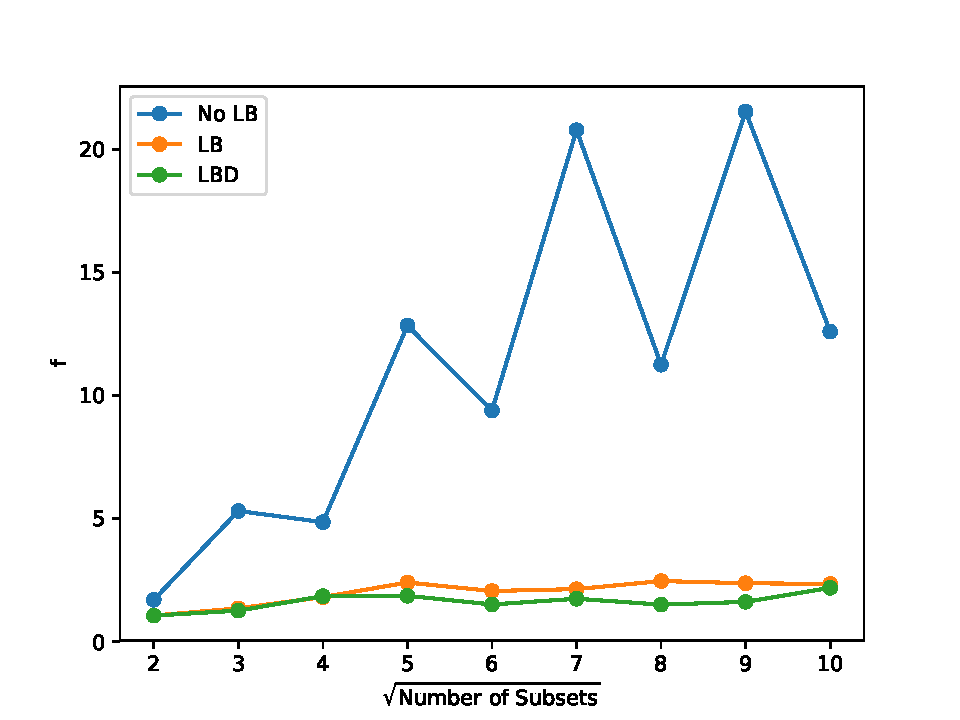
\includegraphics[scale=0.7]{../figures/level2_metric_study.pdf}
\caption{The results of the parametric study with no load balancing, 5 original load balancing iterations, and 5 load-balancing-by-dimension iterations for the Level-2 mesh.}
\label{level2_metric_study}
\end{figure}
\begin{table}[ht]
\centering
\caption{The tabulated results of the parametric study shown in Fig.~\ref{level2_metric_study} with no load balancing, 5 original load balancing iterations (LB), and 5 load-balancing-by-dimension (LBD) iterations for the Level-2 mesh.}
\label{level2_metric_study_table}
\scalebox{0.8}{
\begin{tabular}{c|c|c|c}
\textbf{$\sqrt{\text{Num Subsets}}$} & \bf $f_{\text{reg}}$ & \bf $f_{\text{LB}}$  & \bf $f_{\text{LBD}}$\\ \hline
2&1.7&1.06&1.06\\ \hline
3&5.31&1.35&1.26\\ \hline
4&4.85&1.81&1.85\\ \hline
5&12.83&2.4&1.86\\ \hline
6&9.39&2.06&1.51\\ \hline
7&20.78&2.13&1.74\\ \hline
8&11.25&2.46&1.5\\ \hline
9&21.53&2.37&1.61\\ \hline
10&12.59&2.34&2.18
\end{tabular}}
\end{table}

With regular cut lines going through the Level-2 mesh, $f_\text{reg}$ behaves more erratically than the two pin mesh in Fig.~\ref{partitioning_example}. The natural boundaries are not as uniform, and cells are added in a less consistent fashion. It is noticeable that even numbers of subsets take advantage of the problem's symmetry and consistently have a smaller $f_\text{reg}$ value.

$f_\text{LB}$ and $f_\text{LBD}$ behave much less erratically than $f_\text{reg}$ for the Level-2 mesh.
Table \ref{level2_metric_improvement} shows the percent decrease in $f$ with the original load-balancing algorithm and the load-balancing-by-dimension algorithm relative to no load balancing, and the percent decrease in $f$ with the load-balancing-by-dimension algorithm relative to the original load-balancing algorithm.
Both algorithms can decrease $f$ up to 90\%, but what is notable is the smaller improvement in the load-balancing-by-dimension algorithm relative to the load-balancing-algorithm.
With only one dense feature located in the middle of the mesh, moving the $y$ cut lines on a columnar basis is much less advantageous.
%%%%%%%%%%%%%%
\begin{table}[ht]
\centering
\caption{The percent decrease of $f$ with the original load balancing algorithm (LB) and the load-balancing-by-dimension algorithm (LBD) relative to no load balancing, and the percent decrease of $f$ with the load-balancing-by-dimension algorithm relative to the original load balancing algorithm for the Level-2 mesh.}
\label{level2_metric_improvement}
\begin{tabular}{c|c|c|c}
\textbf{$\sqrt{\text{Num Subsets}}$} & \bf LB v. Regular  & \bf LBD v. Regular & \bf LBD v. LB \\ \hline
2&37.88\%&37.88\%&0.0\%\\ \hline
3&74.56\%&76.29\%&6.8\%\\ \hline
4&62.74\%&61.95\%&-2.11\%\\ \hline
5&81.3\%&85.51\%&22.53\%\\ \hline
6&78.11\%&83.95\%&26.66\%\\ \hline
7&89.74\%&91.62\%&18.33\%\\ \hline
8&78.13\%&86.65\%&38.96\%\\ \hline
9&88.99\%&92.51\%&31.96\%\\ \hline
10&81.41\%&82.66\%&6.71\%
\end{tabular}
\end{table}

\FloatBarrier
The unstructured meshing capability in PDT allows the user to solve a wider variety of problems, without the need to conform a geometry to a logically Cartesian mesh.
The original load balancing and load-balancing-by-dimension algorithms allowed for these unstructured problems to be run more efficiently on large numbers of processors.
However, PDT's performance model does not account for unstructured meshes or imbalanced partitions, but rather assumes a structured grid with an equivalent amount of cells per processor.
In addition, theoretical studies showed that well balanced partitions when using the load-balancing-by-dimension algorithm did not always translate to a better sweep time.
These two reasons motivated the development of a time-to-solution estimator that can estimate the sweep time for a problem given a partitioning scheme ($P_i, A_i$) regardless of mesh type. The time-to-solution estimator is described in Chapter \ref{cha:tts}.

%%%%%%%%%%%%%%%%%%%%%%%%%%%%%%%%%%%%%%%%%%%%%%%%%%%%%%%%%%%%%%%%%%%%%%%%%%%%%%%%%%%
%%%%%%%%%%%%%%%%%%%%%%%%%%%%%%%%%%%%%%%%%%%%%%%%%%%%%%%%%%%%%%%%%%%%%%%%%%%%%%%%%%%
\section{The time-to-solution estimator}\label{cha:tts}
%%%%%%%%%%%%%%%%%%%%%%%%%%%%%%%%%%%%%%%%%%%%%%%%%%%%%%%%%%%%%%%%%%%%%%%%%%%%%%%%%%%
%%%%%%%%%%%%%%%%%%%%%%%%%%%%%%%%%%%%%%%%%%%%%%%%%%%%%%%%%%%%%%%%%%%%%%%%%%%%%%%%%%%
\tcr{You have 38 pages from here on out. Way too many... First, we need a new name for this Section. How about: A time-to-solution weighted approach to partitioning on unstructured grids.
\begin{enumerate}
\item General ideas of what we want to do. Again, it kind introduces the other subsections.
\item Weighted task-dependent graphs for unstructured grid partitioning. Here, you first talk about the TDG and why/how to weight them. Then onto some of the details of the time-to-solution estimator. However, you say way too much. to guide you, I think the following figures need to be yanked out: 13, 14, 15, 16, (not sure about 17 but if we can convey the meaning without a visual aid, yes, remove it), 18, 19, 20, 21, 22. So that's a lot of figures out. This should tell you that a lot of condensing is to happen so extract the essence of the method, not every single detail as in a thesis/dissertation. I think Fig. 24 is not useful either, so out. Likewise for Fig. 25. Maybe 26 can stay. 
\item So the previous section should have appropriate sub-sections. I didn't work them out. Please take a crack at those subsections.
\item After that, you should have a Results subsection that discusses some of the results, before we move on tot he last Section (optimization strategies). Here are some result figures that are NOT necessary: 28, 30 (not all graphs in 29,31, 33 are needed either), 32, 34, 35. If you jsut state how that verification was done (uniformly weighted graph which should be exactly = tp PDT's perf model and it was; that's good enough. A sample of the grid types, not 4 graphs per type, is enough as well). result you should keep: fig 36--38. not sure about 39--43, maybe only 41--43 only?.  
\end{enumerate}
I think this should be no more than 5-6 pages. Currently, from 3.4 until section 4 (excluded), you have 11 pages.
}


With the introduction of unstructured meshes and imbalanced partitions in PDT, we need an expansion of the performance model to estimate the sweep time.
In addition, before optimization of the partitioning scheme can occur, it is necessary to have an estimation tool that gives the approximate sweep time for a given partitioning scheme.
The time-to-solution estimator serves as the objective function that gets optimized, with the partitions serving as the parameter space. This chapter will detail the time-to-solution estimator, and showcase the results of 2D and 3D verification studies.

The time-to-solution estimator is written in Python 3. Python was chosen as the language for its powerful graph library, networkx \cite{networkx}.
This library gives us a wide variety of graph mathematics and is easy to use.
Before detailing the time-to-solution estimator's methodology, a description of the applicable basic graph theory is necessary.

%%%%%%%%%%%%%%%%%%%%%%%%%%%%%%%%%%%%%%%%%%%%%%%%%%%%%%%%%%%%%%%%%%%%%%%%%%%%%%%%%%%
\subsection{Graph Theory Applicable to the Time-to-Solution Estimator}
%%%%%%%%%%%%%%%%%%%%%%%%%%%%%%%%%%%%%%%%%%%%%%%%%%%%%%%%%%%%%%%%%%%%%%%%%%%%%%%%%%%

Graph theory is a subset of mathematics that focuses on graphs, or structures containing a set of objects that are connected in a particular manner \cite{graphtheory}.
These objects are called vertices (or nodes), and are connected by edges.
Figure~\ref{basic_graph} shows an undirected graph of 4 nodes and 4 edges. The nodes are a mathematical abstraction that can be used to represent a variety of concepts. In this dissertation, they are used to represent the subsets described in Chapter \ref{cha:lb}.
\begin{figure}[H]
\centering
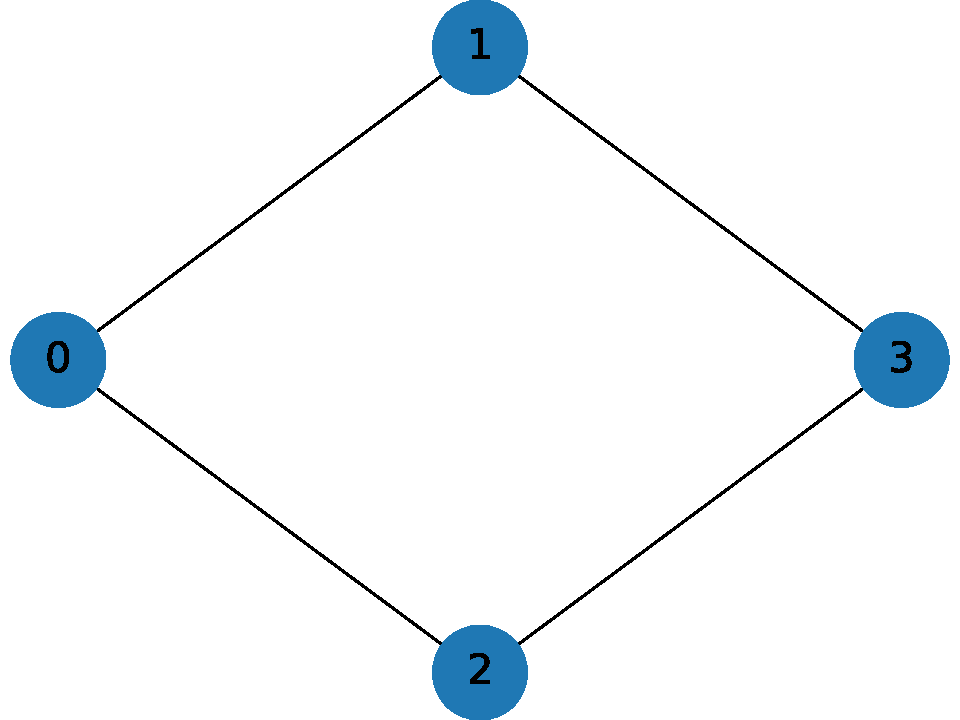
\includegraphics[scale=0.5]{../figures/undirected_graph.pdf}
\caption{An undirected graph with 4 nodes and 4 edges. }
\label{basic_graph}
\end{figure}
Figure~\ref{basic_graph} is referred to as an undirected graph because its edges have no directional information.
If we add directional information to the edges of the graph in Fig.~\ref{basic_graph}, it becomes a directed graph, shown in Fig.~\ref{directed_graph}.
\begin{figure}[H]
\centering
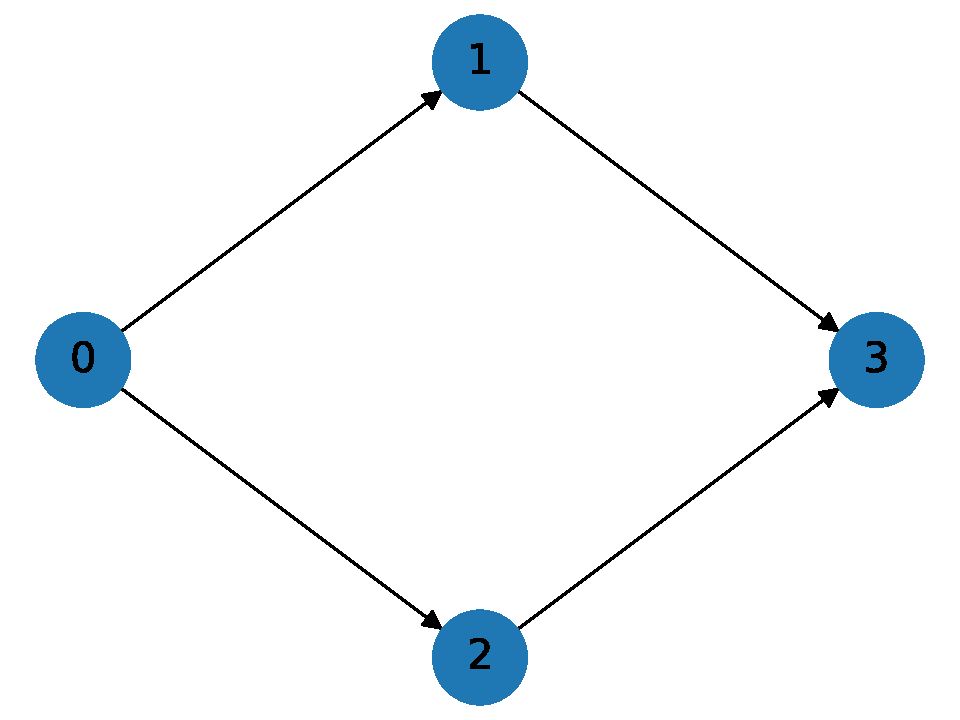
\includegraphics[scale=0.5]{../figures/directed_graph.pdf}
\caption{A directed graph with 4 nodes and 4 edges. }
\label{directed_graph}
\end{figure}
In this dissertation, we only use Directed Acyclic Graphs (DAGs), or a graph that has no cycles.  A cycle is defined as a path on a graph that starts and ends at the same vertex. Figure~\ref{cycle_example} shows a cycle between nodes 1 and 3.
\begin{figure}[H]
\centering
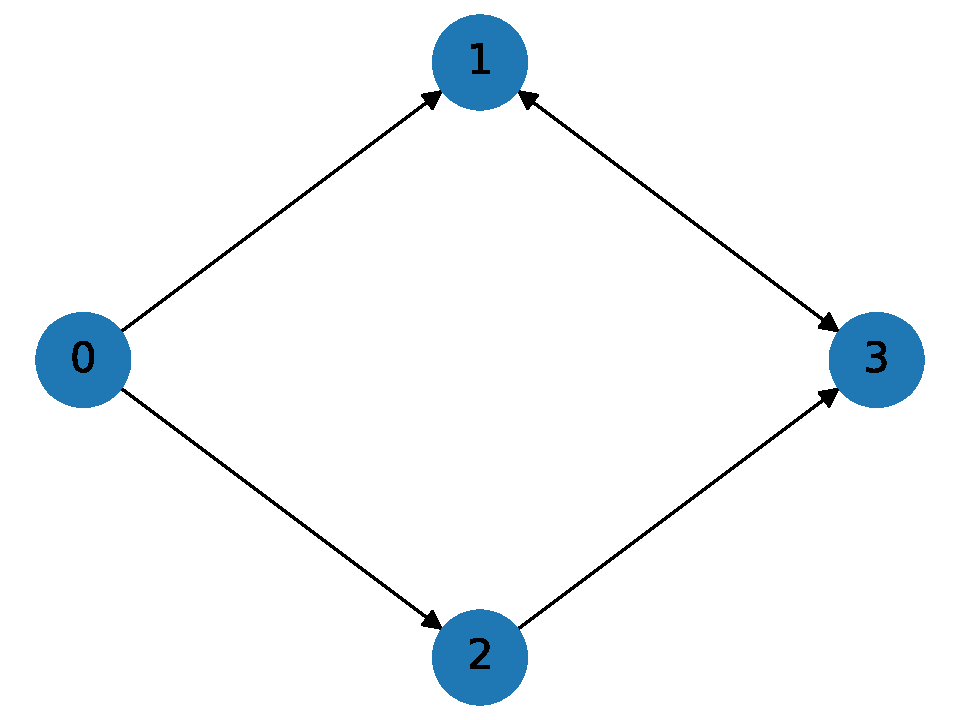
\includegraphics[scale=0.5]{../figures/cycle_example.pdf}
\caption{A directed graph with a cycle between nodes 1 and 3.}
\label{cycle_example}
\end{figure}
We notice the edge connecting nodes 1 and 3 has a double headed arrow, representing a cycle.
Graphs with cycles can be solved for a variety of applications through the use of cycle detection and breaking algorithms, but our partitioning scheme cuts subsets in a fashion that does not allow for cyclical graphs.

Graph edges can be weighted based on the need of the application the graph is being used for. Here, we weight the graph edges to represent the time it takes to solve node A plus the communication time to node B.
Figure~\ref{weighted_directed_graph} shows a weighted directed graph.
In the context of the time-to-solution estimator, subset 1 takes 3 seconds to solve and communicate to subset 3.
\begin{figure}[H]
\centering
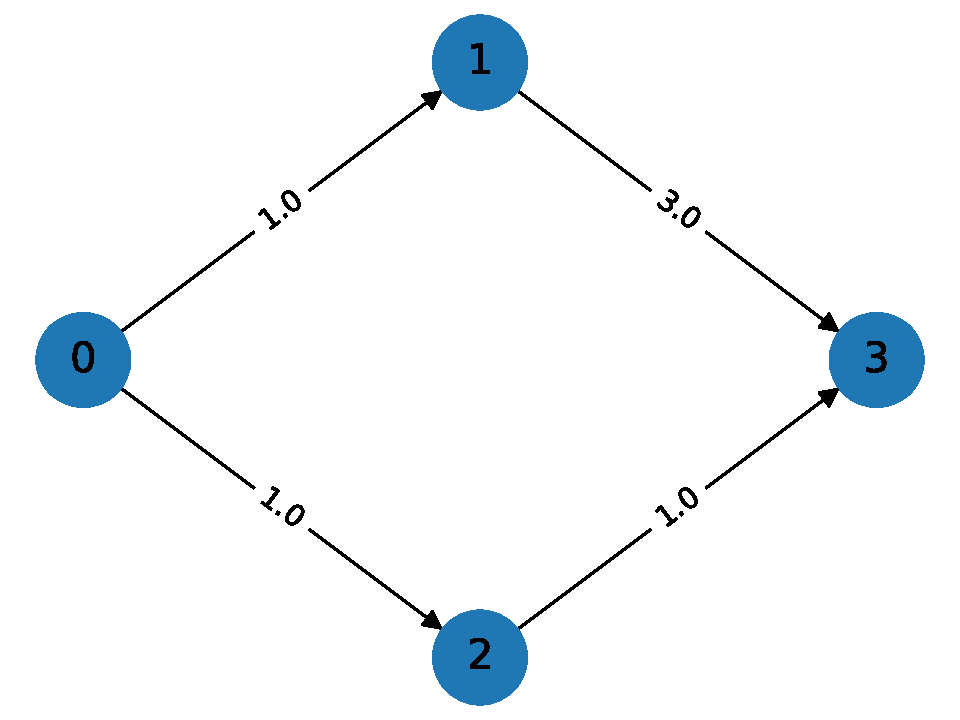
\includegraphics[scale=0.5]{../figures/weighted_directed_graph.pdf}
\caption{A weighted directed acyclic graph with 4 nodes and 4 weighted edges.}
\label{weighted_directed_graph}
\end{figure}

The time-to-solution estimator uses Johnson's algorithm \cite{intro_to_alg,johnson_nist,johnson_johnson} to find all shortest paths between all pairs in a weighted directed graph.
The weighted shortest path is defined as the path between two nodes that has the smallest weighted sum.
For example, the shortest path between nodes 0 and 3 in Fig.~\ref{weighted_directed_graph} is $0\rightarrow 2\rightarrow 3$.

In our application, we use Johnson's algorithm to assist in calculating the longest path between two nodes in a DAG (needed in Section \ref{sec:universal}).
The longest path is found by:
\begin{enumerate}
  \item Multiplying all edge weights by -1,
  \item Using Johnson's algorithm to find the shortest (in this case the most negative) paths,
  \item Summing the original weights of this shortest path.
\end{enumerate}
Johnson's algorithm is specifically used in this process because it is capable of finding the shortest path even when edge weights are negative.

%In addition to longest path length calculation, we use an unweighted shortest path algorithm when calculating the depth-of-graph remaining (needed in Section \ref{sec:conflict}).

%\begin{figure}[H]
%\centering
%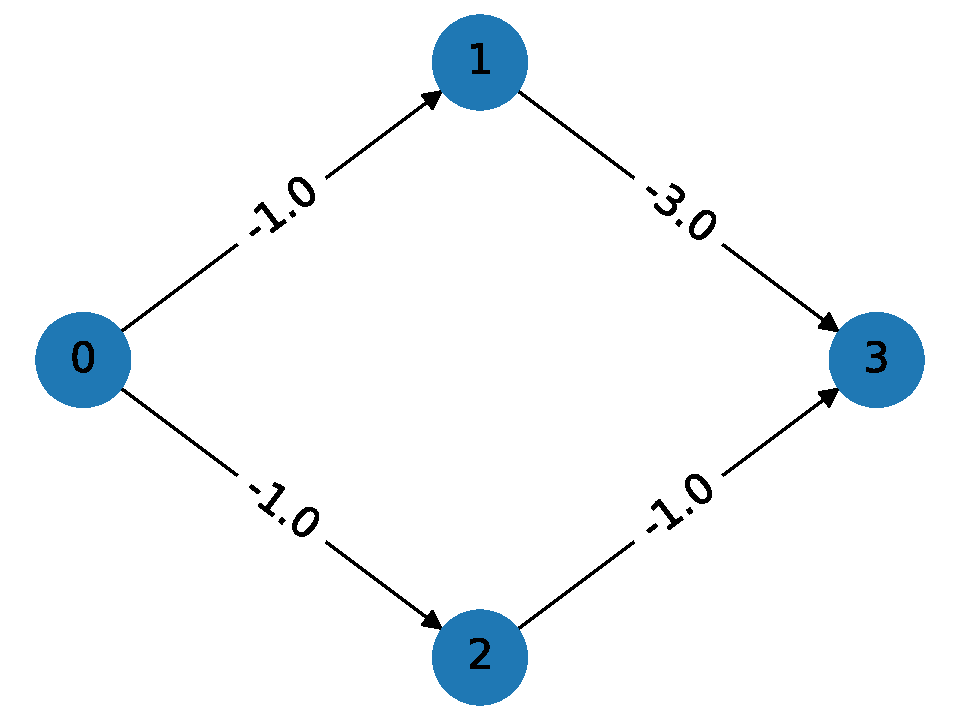
\includegraphics[scale=0.5]{../figures/negative_weighted_directed_graph.pdf}
%\caption{The DAG in Fig.~\ref{
%\label{negative_weights}
%\end{figure}
Now that the applicable graph theory has been reviewed, we detail the methodology of the time-to-solution estimator.

%%%%%%%%%%%%%%%%%%%%%%%%%%%%%%%%%%%%%%%%%%%%%%%%%%%%%%%%%%%%%%%%%
\subsection{Method}
%%%%%%%%%%%%%%%%%%%%%%%%%%%%%%%%%%%%%%%%%%%%%%%%%%%%%%%%%%%%%%%%%%%%%%%%%%%%%%%%%%%
The time-to-solution estimator determines the time to sweep across a domain for a given partitioning scheme by:
\begin{enumerate}
	\item Building an adjacency matrix,
	\item Building Directed Acyclic Graphs (DAGs) from the adjacency matrix, one for each quadrant/octant,
	\item Weighting the edges of each graph based on the solve time and communication time of each subset to its neighbors,
     \item Adding and modifying graph weights based on how many anglesets are pipelined,
	\item Modifying the weights of each graph to operate on the universal timescale,
	\item Modifying the weights of each graph to reflect sweep conflicts between octants,
	\item Calculating the time to solution.
\end{enumerate}

%%%%%%%%%%%%%%%%%%%%%%%%%%%%%%%%%%%%%%%%%%%%%%%%%%%%%%%%%%%%%%%%%%%%%%%%%%%%%%%%%%%
\subsubsection{Building the adjacency matrices}
%%%%%%%%%%%%%%%%%%%%%%%%%%%%%%%%%%%%%%%%%%%%%%%%%%%%%%%%%%%%%%%%%%%%%%%%%%%%%%%%%%%

Before building the graph for each quadrant/octant, an adjacency matrix must be built for a given partitioning scheme. The partitioning scheme is the cut lines/planes that partition the mesh into subsets, which correspond to the processor layout.
The adjacency matrix provides connectivity information for each subset to its neighboring subset.
The adjacency building process relies on a major assumption: the z dimension has partitions all the way across the domain, then the x dimension has partitions per plane, then the y dimension has partitions per plane per column.
In future work, these three dimensions can be made interchangeable, but in the present work, this ordering is fixed.

Figure~\ref{25basematrix} shows a partitioning scheme for 3 subsets each in the x and y dimensions with its corresponding adjacency matrix.

\begin{figure}[H]
\begin{minipage}[c]{0.5\textwidth}
\centering
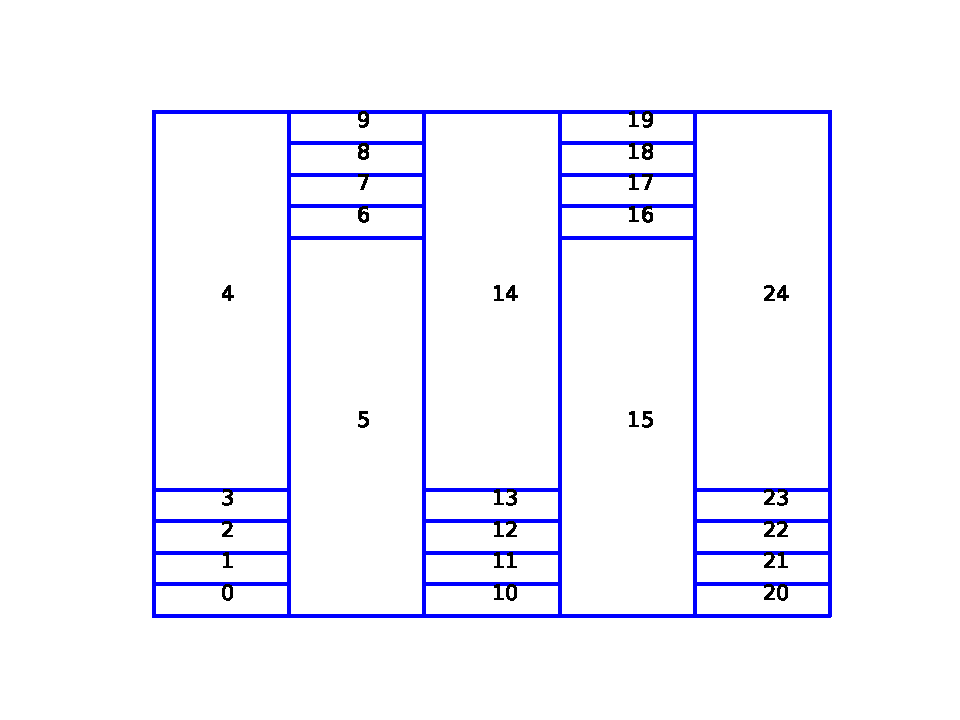
\includegraphics[scale=0.7]{../figures/boundaries_worst.pdf}
\end{minipage}
\begin{minipage}[c]{0.6\textwidth}
\centering
\scalebox{0.75}{
$\begin{pmatrix}
0&1&0&1&0&0&0&0&0\\
1&0&1&1&0&0&0&0&0\\
0&1&0&1&1&1&0&0&0\\
1&1&1&0&1&0&1&1&1\\
0&0&1&1&0&1&0&0&1\\
0&0&1&0&1&0&0&0&1\\
0&0&0&1&0&0&0&1&0\\
0&0&0&1&0&0&1&0&1\\
0&0&0&1&1&1&0&1&0\\
\end{pmatrix}$}
\end{minipage}
\caption{A 3x3 subset partitioning scheme and its corresponding adjacency matrix.}
\label{25basematrix}
\end{figure}

%%%%%%%%%%%%%%%%%%%%%%%%%%%%%%%%%%%%%%%%%%%%%%%%%%%%%%%%%%%%%%%%%%%%%%%%%%%%%%%%%%%
\subsubsection{Building the directed acyclic graphs (DAGs)}
%%%%%%%%%%%%%%%%%%%%%%%%%%%%%%%%%%%%%%%%%%%%%%%%%%%%%%%%%%%%%%%%%%%%%%%%%%%%%%%%%%%

The adjacency matrices give us directed connectivity information in order to build our graphs and are built using networkx's DiGraph function to build the DAGs.

In two dimensions, we build four graphs corresponding to four quadrants.
We define the quadrants in the following manner:
\begin{itemize}
  \item Quadrant 0: $\Omega_x > 0$, $\Omega_y > 0$
  \item Quadrant 1: $\Omega_x > 0$, $\Omega_y < 0$
  \item Quadrant 2: $\Omega_x < 0$, $\Omega_y > 0$
  \item Quadrant 3: $\Omega_x < 0$, $\Omega_y < 0$
\end{itemize}
Figure~\ref{quadrant_layout} illustrates this numbering.
\begin{figure}[H]
\centering
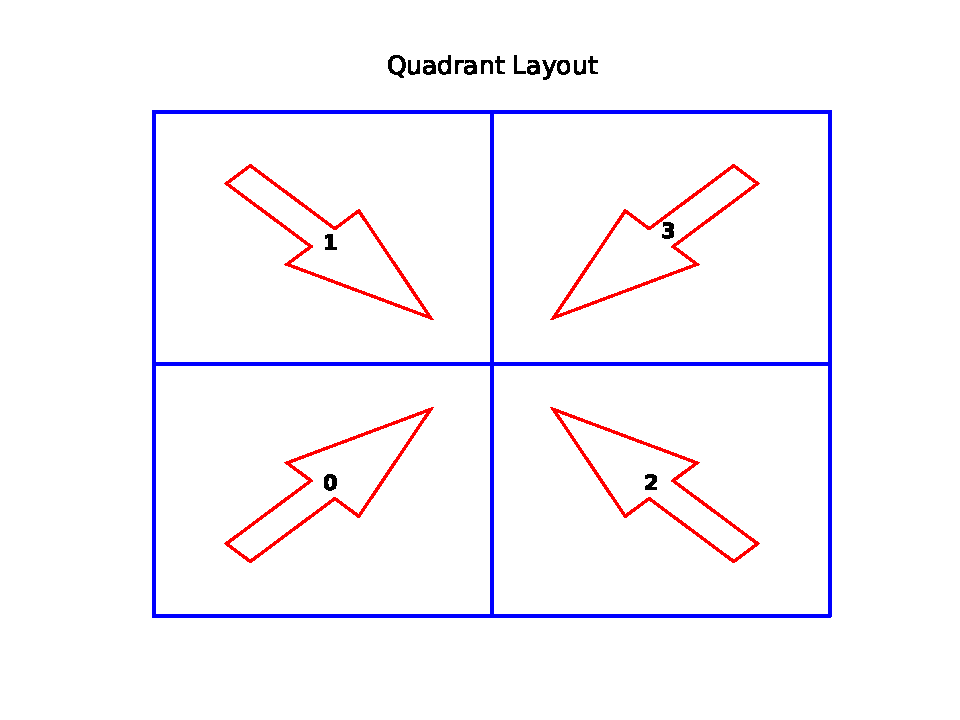
\includegraphics{../figures/quadrant_layout.pdf}
\caption{The quadrant layout for 2D problems.}
\label{quadrant_layout}
\end{figure}
The initial adjacency matrix we obtain can be immediately used to build the graphs for quadrants 0 and 3 by using networkx's DiGraph function.
We feed the upper triangular portion of the adjacency matrix to DiGraph to get the quadrant 0 graph, and the lower triangular portion to get the quadrant 3 graph.
Utilizing the same partitioning scheme shown in Fig.~\ref{25basematrix}, pull the upper triangular and lower triangular portions of the matrix, shown in Fig.~\ref{25baseportionmatrices}.
\begin{figure}[H]
\begin{minipage}[c]{0.5\textwidth}
\centering
\scalebox{0.75}{
$\begin{pmatrix}
0&1&0&1&0&0&0&0&0\\
0&0&1&1&0&0&0&0&0\\
0&0&0&1&1&1&0&0&0\\
0&0&0&0&1&0&1&1&1\\
0&0&0&0&0&1&0&0&1\\
0&0&0&0&0&0&0&0&1\\
0&0&0&0&0&0&0&1&0\\
0&0&0&0&0&0&0&0&1\\
0&0&0&0&0&0&0&0&0\\
\end{pmatrix}$}
\end{minipage}
\begin{minipage}[c]{0.5\textwidth}
\centering
\scalebox{0.75}{
$\begin{pmatrix}
0&0&0&0&0&0&0&0&0\\
1&0&0&0&0&0&0&0&0\\
0&1&0&0&0&0&0&0&0\\
1&1&1&0&0&0&0&0&0\\
0&0&1&1&0&0&0&0&0\\
0&0&1&0&1&0&0&0&0\\
0&0&0&1&0&0&0&0&0\\
0&0&0&1&0&0&1&0&0\\
0&0&0&1&1&1&0&1&0\\
\end{pmatrix}$}
\end{minipage}
\caption{The upper triangular (left) and lower triangular (right) portions of the adjacency matrix in Fig.~\ref{25basematrix}.}
\label{25baseportionmatrices}
\end{figure}
Figure~\ref{25_q0q3graphs} shows the the DAGS associated with quadrants 0 and 3, built from the adjacency matrices in Fig.~\ref{25baseportionmatrices}.
\begin{figure}[H]
\begin{minipage}[c]{0.5\textwidth}
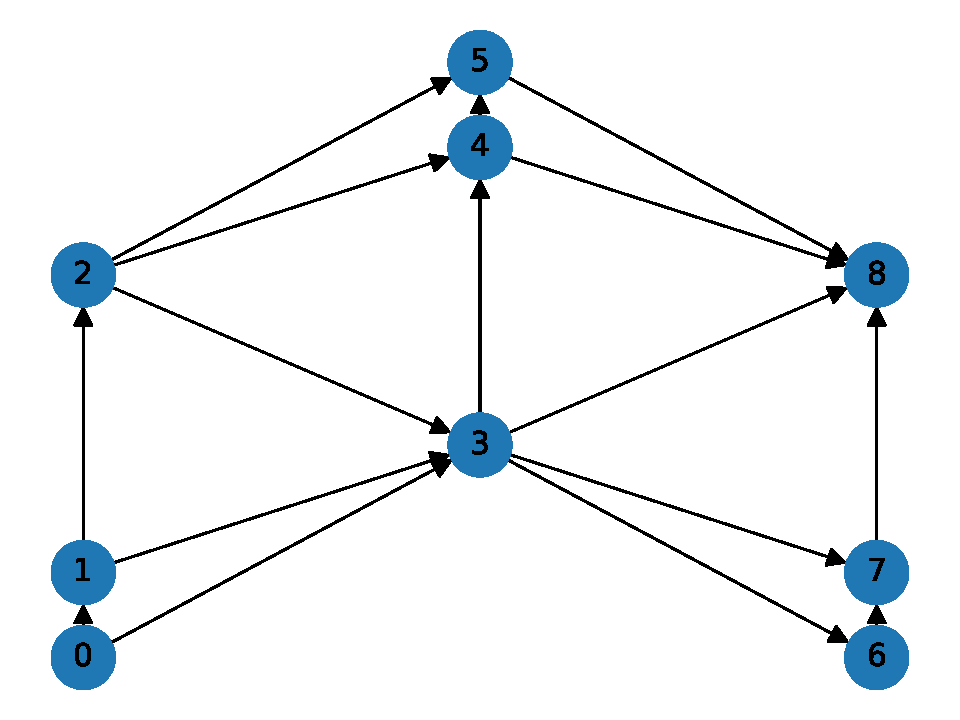
\includegraphics[scale=0.5]{../figures/9_graph0.pdf}
\end{minipage}
\begin{minipage}[c]{0.5\textwidth}
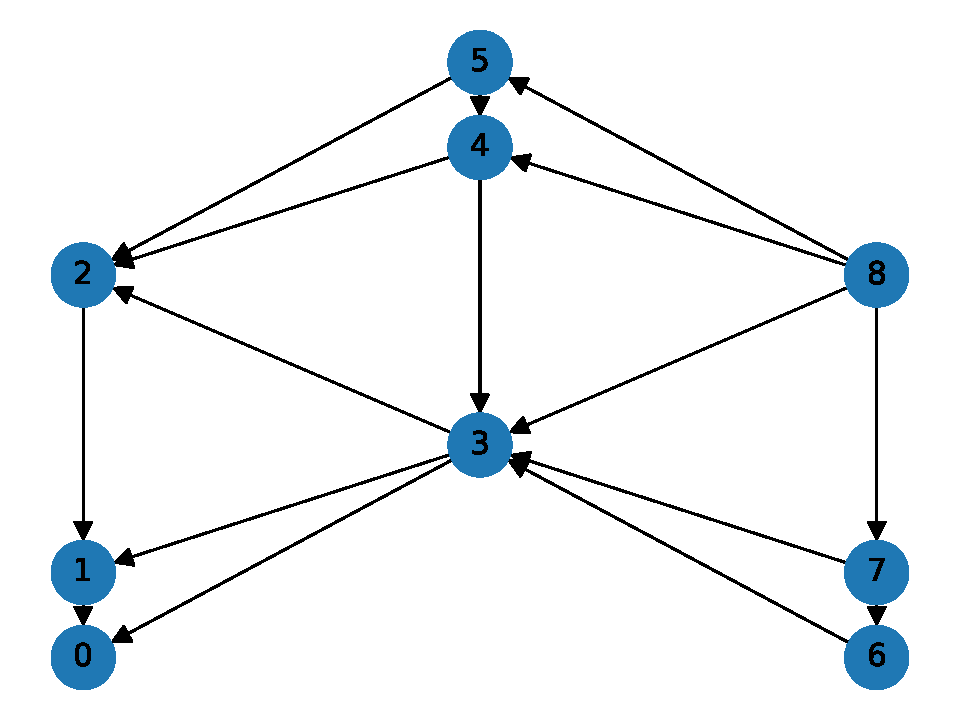
\includegraphics[scale=0.5]{../figures/9_graph3.pdf}
\end{minipage}
\caption{The quadrant 0 DAG (left) and the quadrant 3 DAG (right).}
\label{25_q0q3graphs}
\end{figure}
Upon inspection of these two DAGs, we see that they show the expected connectivity, dependency, and opposing sweep ordering.
Quadrant 0 starts its sweep from subset 0, finishing at subset 8, and quadrant 3 starts its sweep from subset 8, finishing at subset 0.

To obtain the graphs for quadrants 1 and 2, a ``flipped'' version of the adjacency matrix is necessary.
We temporarily renumber the subsets starting from the top left corner, and increasing down each column, as shown in Fig.~\ref{25flippedmatrix}.
\begin{figure}[H]
\begin{minipage}[c]{0.5\textwidth}
\centering
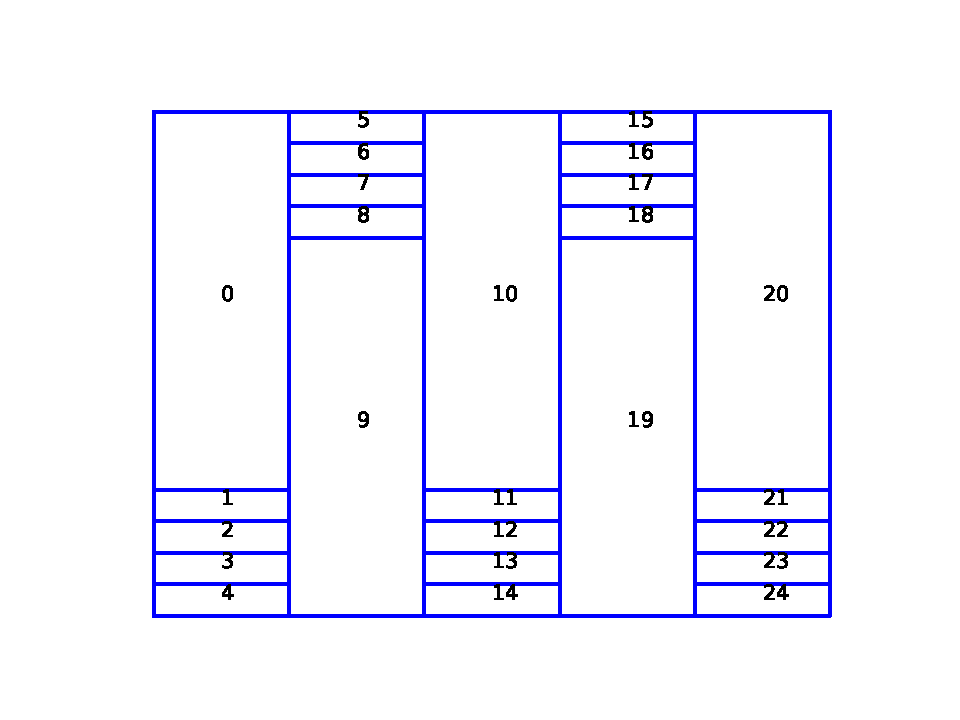
\includegraphics[scale=0.7]{../figures/boundaries_worst_flipped.pdf}
\end{minipage}
\begin{minipage}[c]{0.5\textwidth}
\centering
\scalebox{0.75}{
$\begin{pmatrix}
0&1&0&1&1&1&0&0&0\\
1&0&1&0&0&1&0&0&0\\
0&1&0&0&0&1&0&0&0\\
1&0&0&0&1&0&1&0&0\\
1&0&0&1&0&1&1&0&0\\
1&1&1&0&1&0&1&1&1\\
0&0&0&1&1&1&0&1&0\\
0&0&0&0&0&1&1&0&1\\
0&0&0&0&0&1&0&1&0\\
\end{pmatrix}$}
\end{minipage}
\caption{The flipped subset ordering and corresponding ``flipped'' adjacency matrix for the partitioning scheme in Fig.~\ref{25basematrix}.}
\label{25flippedmatrix}
\end{figure}
We then get the upper triangular and lower triangular portions of the flipped adjacency matrix to get the connectivity and dependency information for quadrants 1 and 2.
We feed the triangular matrices into networkx's DiGraph function, along with a mapping of the flipped subset ids to the original subset ids (shown in Fig.~\ref{25basematrix}). Figure~\ref{25_q1q2graphs} shows the DAGs for quadrants 1 and 2.
\begin{figure}[H]
\begin{minipage}[c]{0.5\textwidth}
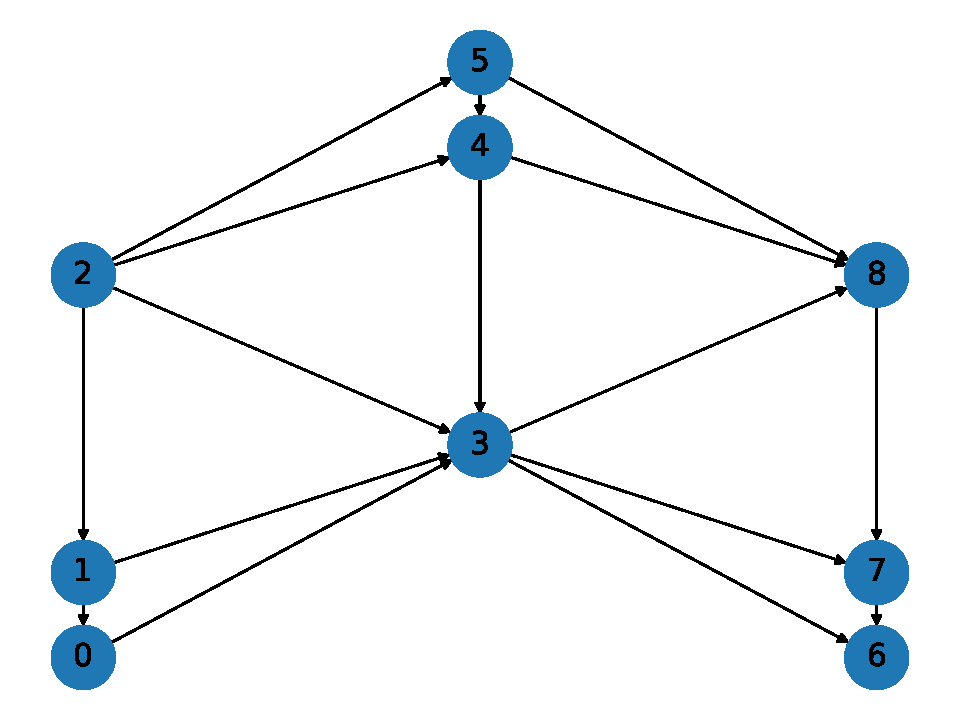
\includegraphics[scale=0.5]{../figures/9_graph1.pdf}
\end{minipage}
\begin{minipage}[c]{0.5\textwidth}
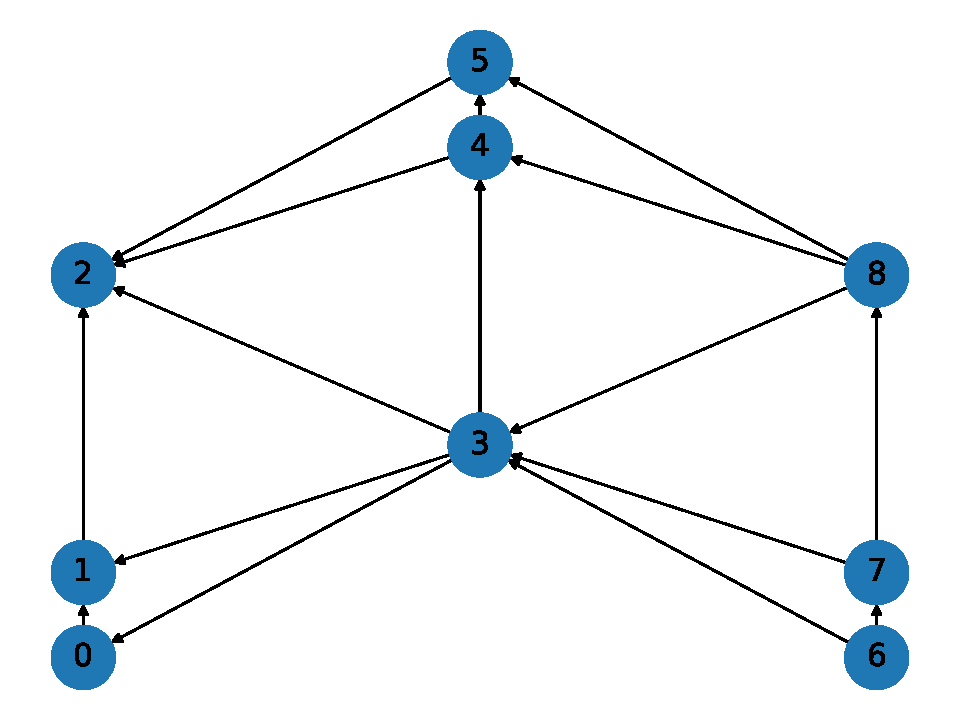
\includegraphics[scale=0.5]{../figures/9_graph2.pdf}
\end{minipage}
\caption{The quadrant 1 DAG (left) and the quadrant 2 DAG(right).}
\label{25_q1q2graphs}
\end{figure}
Upon inspection of these two DAGs, we see that they show the expected connectivity, dependency, and opposing sweep ordering.
Quadrant 1 starts its sweep from subset 2, finishing at subset 6, and quadrant 2 starts its sweep from subset 6, finishing at subset 2.

%Weighting the TDGS
%%%%%%%%%%%%%%%%%%%%%%%%%%%%%%%%%%%%%%%%%%%%%%%%%%%%%%%%%%%%%%%%%%%%%%%%%%%%%%%%%%%
\subsubsection{Weighting the task dependence graphs}
%%%%%%%%%%%%%%%%%%%%%%%%%%%%%%%%%%%%%%%%%%%%%%%%%%%%%%%%%%%%%%%%%%%%%%%%%%%%%%%%%%%

Each graph is weighted to reflect the solve time and communication time of each node to its neighbors. Explicitly, the edge weight between node A and node B represents the solve time of node A added to the time it takes to communicate boundary information from nod A to node B. Equation \ref{weight_function} shows how the weights are calculated:
\begin{equation}
\text{weight} = \text{mcff}\cdot [T_{wu} + N_n\cdot \text{latency}\cdot M_L + T_{\text{comm}}\cdot N_b\cdot A_m\cdot upbc + \cdot N_c\cdot (T_c + A_m\cdot (T_m + T_g))],
\label{weight_function}
\end{equation}
where:
\begin{itemize}
  \item mcff = the Multi-Core Fudge Factor, a corrective factor that accounts for performance drop-off from 1 to 8 cores,
  \item $T_{wu}$ = the time to get into the sweep operator,
  \item $N_n$ = the number of neighbors this node has to communicate to,
  \item latency = the machine specific communication latency,
  \item $M_L$ = the machine specific latency multiplier,
  \item $T_{\text{comm}}$ = the communication time per double,
  \item $N_b$ = the number of boundary cells shared by node A and node B,
  \item $A_m$ = the number of angles node A has to solve prior to communicating,
  \item $upbc$ = the number of boundary unknowns per boundary cell,
  \item $N_c$ = the number of cells in node A,
  \item $T_c$ = the time spent solving cell-specific work,
  \item $T_m$ = the time spent solving angle-specific work,
  \item $T_g$ = the time spent solving group-specific work.
\end{itemize}
The weighting function is based on PDT's performance model \cite{mpadams2013,mpadams2015,mpadamsjcp}, which is specific to how PDT solves the transport sweep. The cost function can be modified based on different sweep methodologies if a user desires.

As shown in Eq. \ref{weight_function}, a crucial part of determining the weight of each edge is knowing the number of cells each subset has, and the amount of shared boundary cells with each neighbor. Given a mesh density, the number of cells per subset is given by Eq \ref{cellspersubset}:
\begin{equation}
   \text{cells per subset} = \int_{x_i}^{x_{i+1}} \int_{y_j}^{y_{j+1}} \int_{z_k}^{z_{k+1}} \text{mesh density } dx dy dz,
\label{cellspersubset}
\end{equation}
where the integral bounds represent the cut plane coordinates that form the subset.
Equations \ref{nxy}-\ref{nyz} calculate the boundary cells along each face in 3D:
\begin{align}
n_{xy} &= \Big(\frac{N_c}{V}\Big)^{2/3}\cdot L_x\cdot L_y \label{nxy}, \\
n_{xz} &= \Big(\frac{N_c}{V}\Big)^{2/3}\cdot L_x\cdot L_z \label{nxz}, \\
n_{yz} &= \Big(\frac{N_c}{V}\Big)^{2/3}\cdot L_y\cdot L_z \label{nyz},
\end{align}
where $N_c$ is the number of cells in the subset, $V$ is the subset volume, and $L_d$ is the length of the subset in dimension $d$.
Equations \ref{nx} and \ref{ny} show the 2-dimensional equivalents to \ref{nxy}-\ref{nyz}:
\begin{align}
n_x &= \Big(\frac{N_c}{A}\Big)^{1/2}\cdot L_x, \label{nx} \\
n_y &= \Big(\frac{N_c}{A}\Big)^{1/2}\cdot L_y, \label{ny}
\end{align}
where $A$ is the subset area. Equations \ref{cellspersubset}-\ref{ny} are exact for structured meshes.
However, unstructured meshes do not necessarily have an easily integrable mesh density function to calculate the cells per subset.

To get the cells per subset for unstructured meshes we require the vertex data of the mesh, as well as which vertices form each cell in the mesh.
With this data, we take advantage of Python's shapely library \cite{shapely} to determine which cells lie in each subset. From the vertex and cell data of the mesh, we build a lightweight version of each cell as a shapely Polygon.\\
\noindent
For each subset we:
\begin{enumerate}
  \item Loop over the Polygons.
  \item For each polygon, check if the Polygon is within the subset. If it is, add it to the cells in that subset.
  \item If it is not within the subset, check if the Polygon intersects the subset.
  \item If it does intersect the subset, check if it lies on a natural boundary and is outside the subset.
  \item If it is not on a natural boundary and truly intersects the subset, then this Polygon's intersection with the subset forms a new cell,  and is added to the total number of cells in that subset.
\end{enumerate}
%%%%%%%%%%Table
Table \ref{2x2_cellcount} tabulates the cells count per subset for the time-to-solution estimator and PDT for the mesh in Fig.~\ref{partitioning_example} partitioned into 2 subsets in each dimension with regular cuts.
\begin{table}[H]
\centering
\caption{The cell count per subset for the time-to-solution estimator and PDT for the mesh in Fig.~\ref{partitioning_example} partitioned into 2 subsets in each dimension with regular cuts.}
\label{2x2_cellcount}
\begin{tabular}{c|c|c}
\textbf{Subset} & \textbf{Cell Count TTS} & \textbf{Cell Count PDT} \\ \hline
0 & 185 & 185 \\ \hline
1 & 25 & 25 \\ \hline
2 & 25 & 25 \\ \hline
3 & 185 & 185
\end{tabular}
\end{table}

Figure~\ref{ubp_7x7} shows the mesh in Fig.~\ref{partitioning_example} partitioned into 7 subsets in each dimension with load-balanced-by-dimension cuts. This mesh has many subsets that slice through cells, creating new cells. Figure~\ref{cell_comp} shows the cell counts per subset from PDT and the time-to-solution estimator are in perfect agreement.
%%%%%%%%%%%%%%%%%
\begin{figure}[H]
\centering
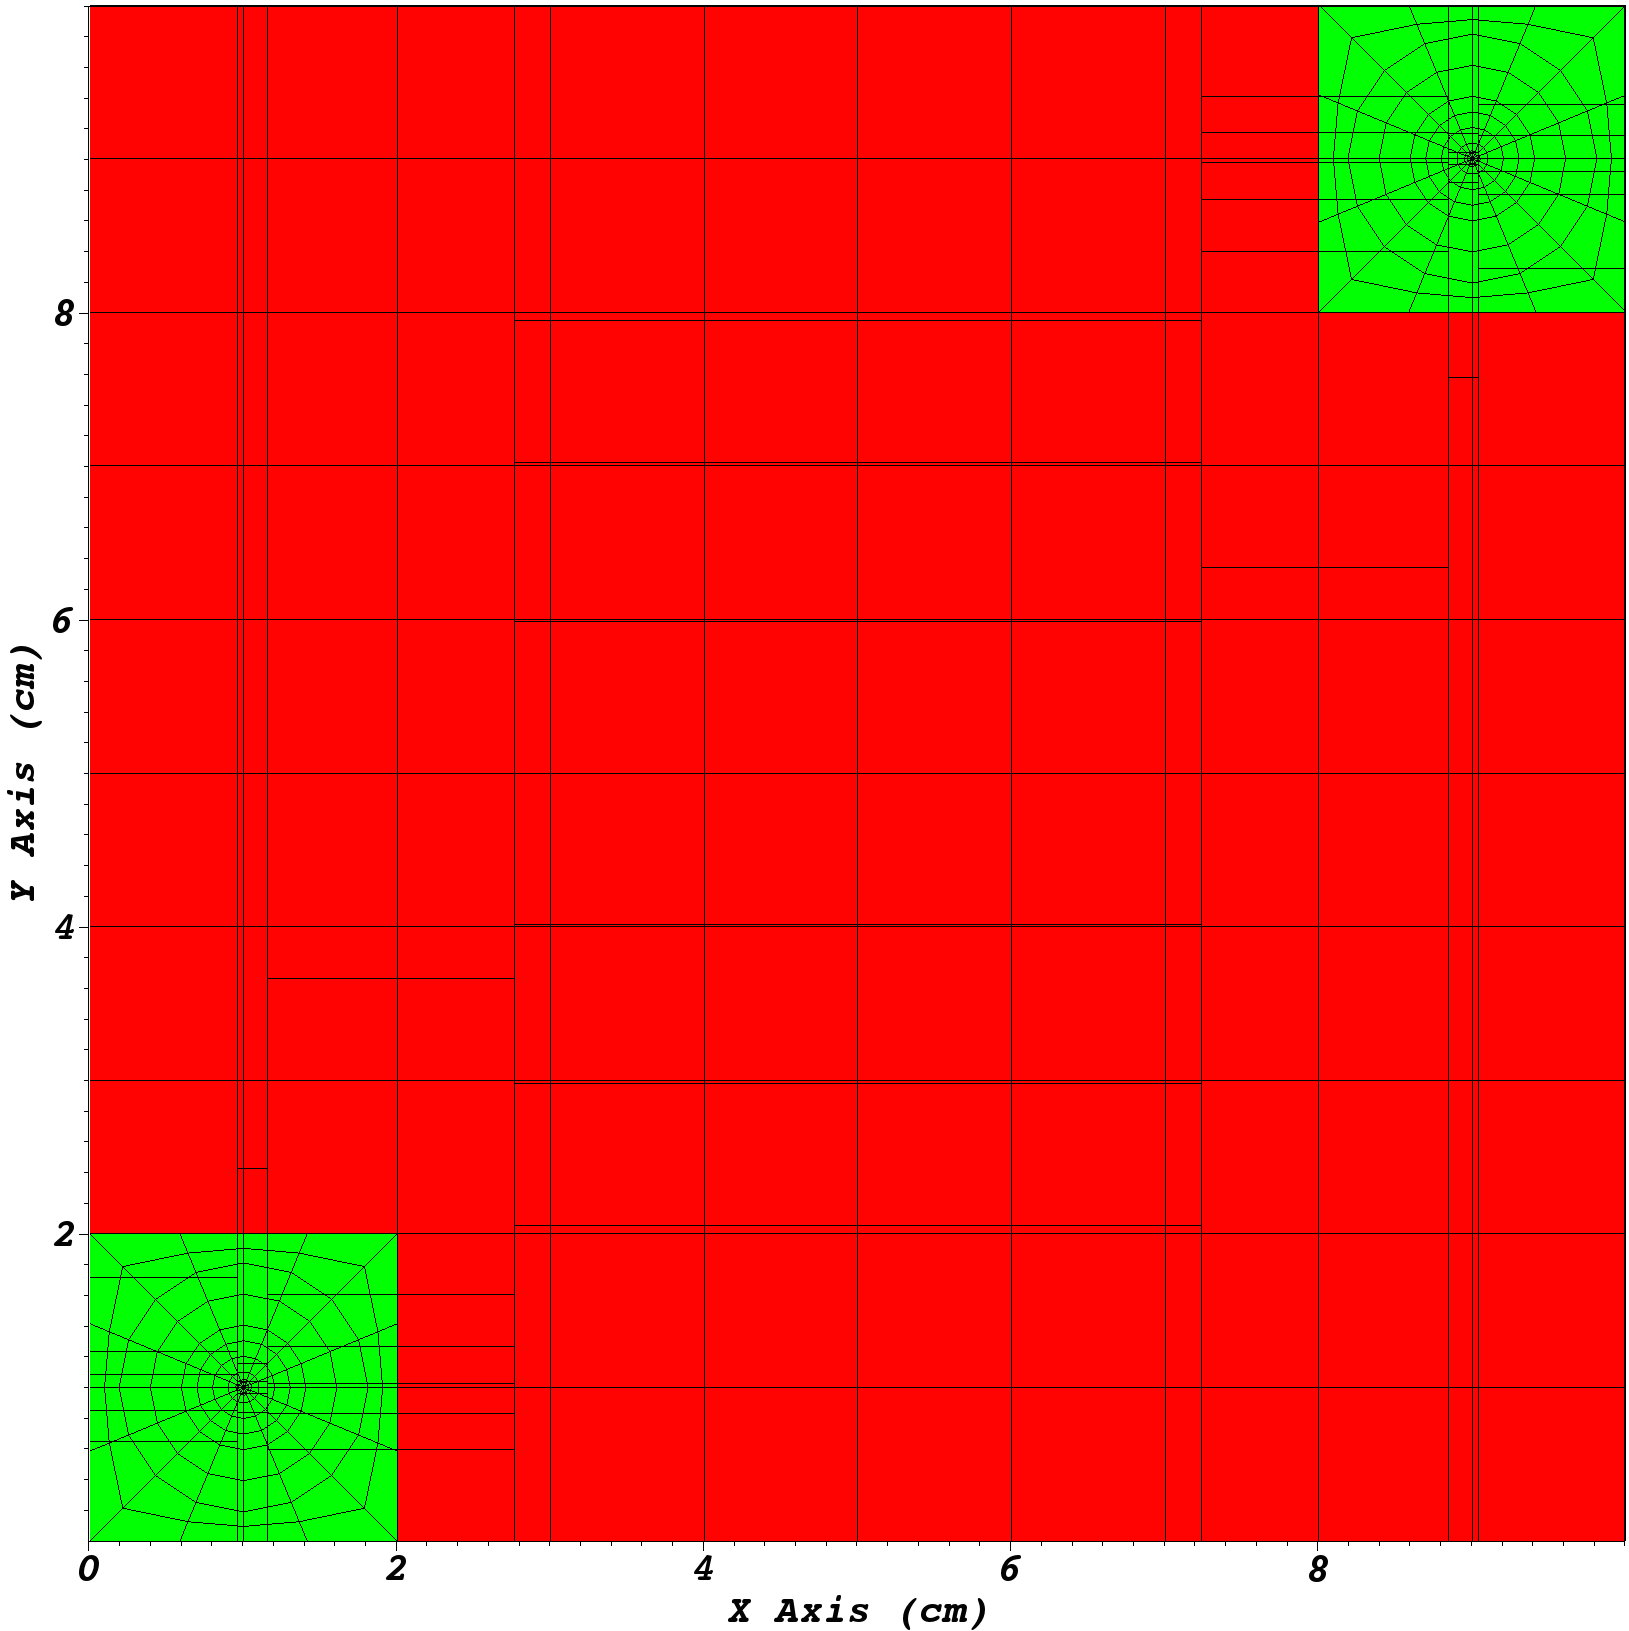
\includegraphics[scale=0.15]{../figures/spiderweb_7x7_lbd.png}
\caption{The mesh in Fig.~\ref{partitioning_example} partitioned into 7 subsets in each dimension with load-balanced-by-dimension cuts. $f = 1.49$}
\label{ubp_7x7}
\end{figure}
\begin{figure}[H]
\centering
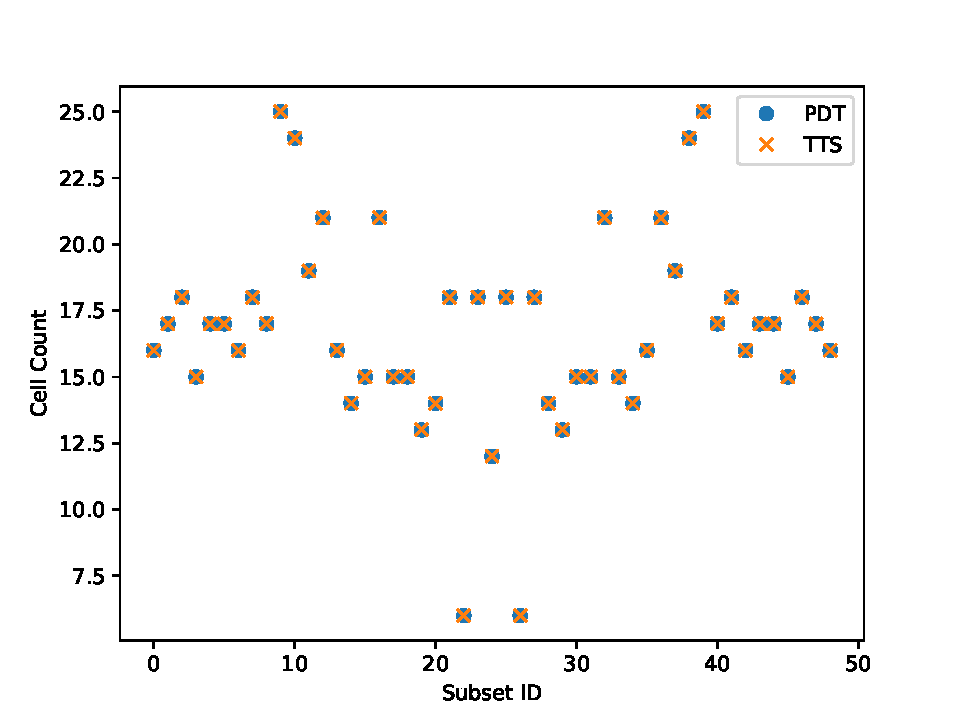
\includegraphics[scale=0.75]{../figures/spiderweb_cell_comp_7x7.pdf}
\caption{The cell count per subset for the mesh in Fig.~\ref{ubp_7x7} from PDT and the time-to-solution estimator.}
\label{cell_comp}
\end{figure}

With confidence in the cell count per subset in the time-to-solution estimator matching PDT, we make an assumption that the cells in each subset are close to uniformly distributed. This allows us to continue to use Eqs. \ref{nxy}-\ref{ny} to calculate the boundary cells in each subset.

With this information, we compute all weights in each graph according to Eq. \ref{weight_function}.
Once graphs are weighted, we add and modify edge weights for the number of angles pipelined per octant/quadrant.

%%%%%%%%%%%%%%%%%%%%%%%%%%%%%%%%%%%%%%%%%%%%%%%%%%%%%%%%%%%%%%%%%%%%%%%%%%%%%%%%%%%
\subsubsection{Adding graphs for angular pipelining}
%%%%%%%%%%%%%%%%%%%%%%%%%%%%%%%%%%%%%%%%%%%%%%%%%%%%%%%%%%%%%%%%%%%%%%%%%%%%%%%%%%%

If there are angles to be pipelined, the time-to-solution estimator adds a new set of graphs for each additional angle to be pipelined. For example, if there are two anglesets per octant, this would results in 16 graphs, or 1 graph per octant per angleset. Figure~\ref{angular_pipeline} shows the graphs for two anglesets for a quadrant. A ``dummy'' node with a value of -2 is added in order to have an incoming edge for the first subset's node. The value of this incoming edge represents when that angleset starts its sweep.
\begin{figure}[H]
\begin{minipage}[c]{0.5\textwidth}
\centering
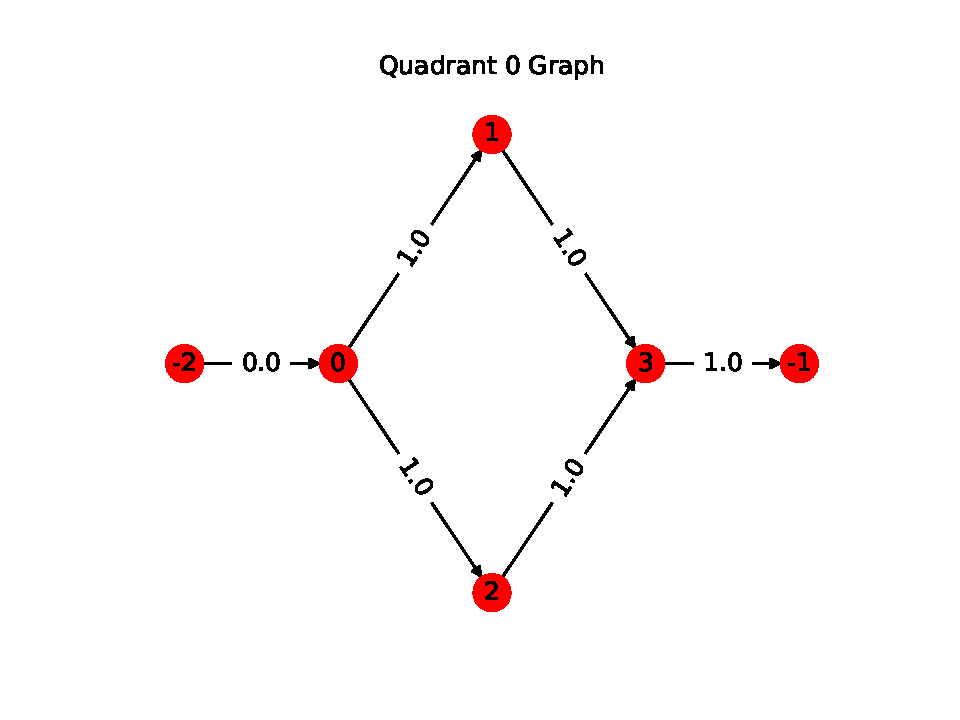
\includegraphics[scale=0.6]{../figures/q0_postpipeline.pdf}
\end{minipage}
\begin{minipage}[c]{0.5\textwidth}
\centering
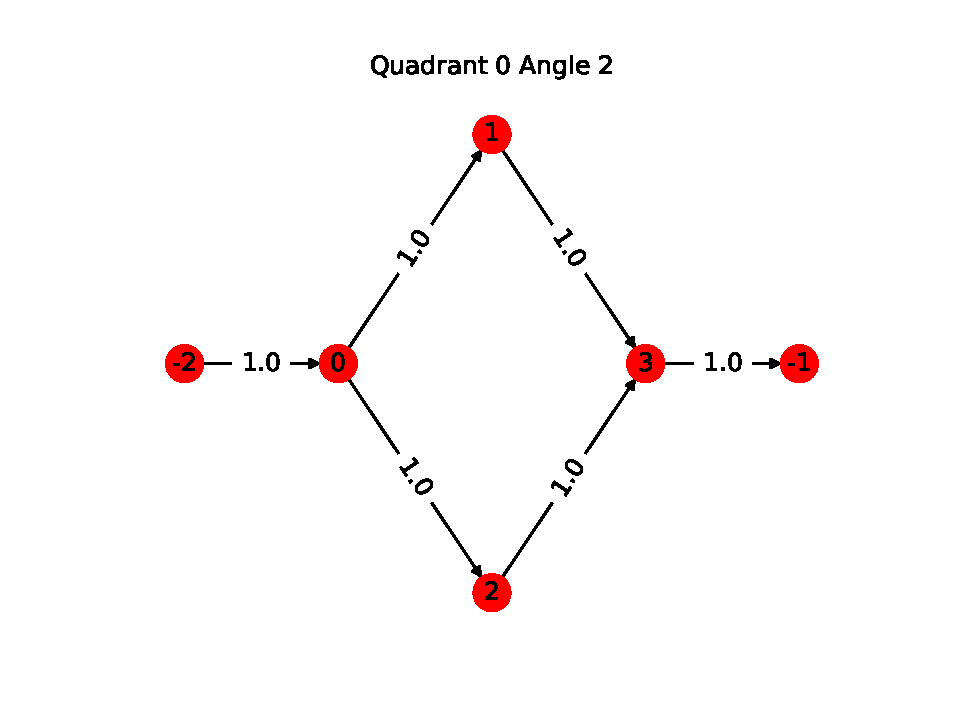
\includegraphics[scale=0.6]{../figures/q4_postpipeline.pdf}
\end{minipage}
\caption{The graphs for the first (left) and second (right) anglesets}
\label{angular_pipeline}
\end{figure}

%%%%%%%%%%%%%%%%%%%%%%%%%%%%%%%%%%%%%%%%%%%%%%%%%%%%%%%%%%%%%%%%%%%%%%%%%%%%%%%%%%%
\subsubsection{Modifying the weights of each graph to reflect a universal timescale}\label{sec:universal}
%%%%%%%%%%%%%%%%%%%%%%%%%%%%%%%%%%%%%%%%%%%%%%%%%%%%%%%%%%%%%%%%%%%%%%%%%%%%%%%%%%%

Once we have our full set of graphs with angular pipelining accounted for, we set up each graph to reflect a universal timescale, with the goal of knowing when each node in each graph is ready to solve.
For each node in each graph, we:
\begin{enumerate}
  \item Calculate the longest path to the node,
  \item Sum the weights of the edges along the longest path,
  \item Set all incoming edge values to the node to the sum of the longest path.
\end{enumerate}
The incoming edges to each node in each graph now reflect the time at which a node is ready to solve. This universal edge weighting is used for detecting and resolving conflicts during the sweep. It is important to note that our DAGs are now task dependence graphs (TDGs). We now know which node is ready to solve at each time $t$, which provides us with a schedule. Figure~\ref{universal} shows a simple example of a DAG becoming a TDG.
\begin{figure}[H]
  \begin{minipage}[c]{0.5\textwidth}
    \centering
    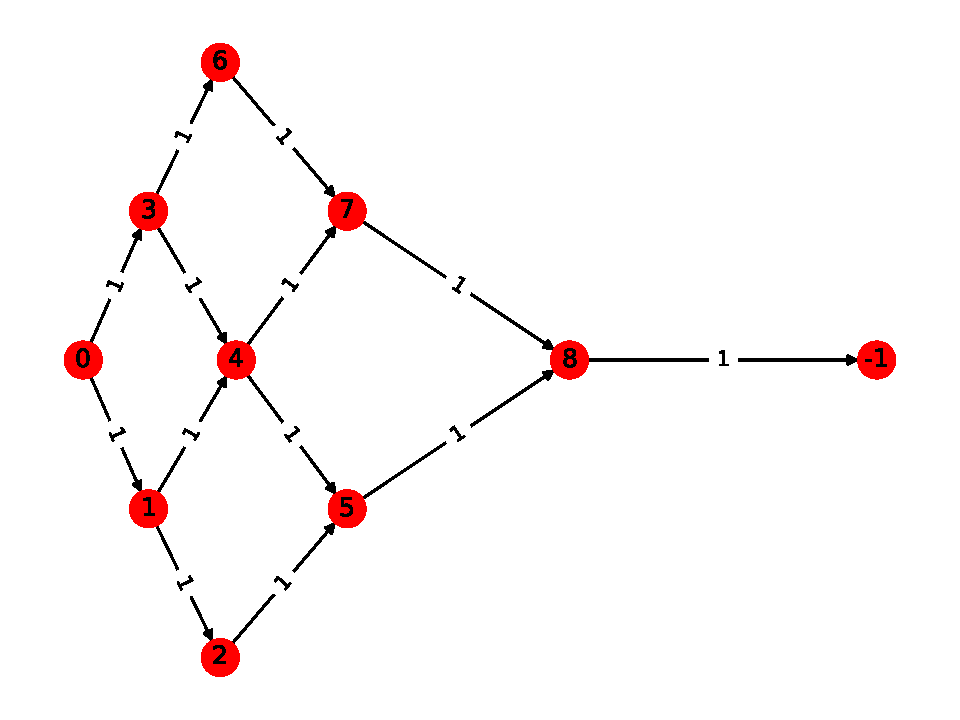
\includegraphics[scale=0.5]{../figures/G_pre_universal.pdf}
  \end{minipage}
  \begin{minipage}[c]{0.5\textwidth}
    \centering
    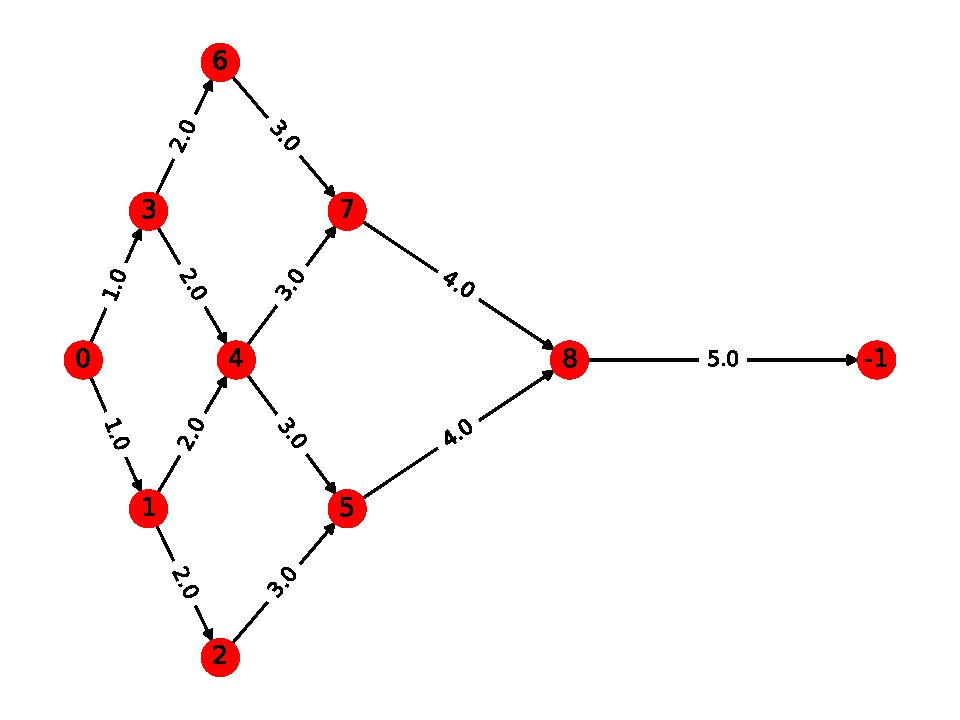
\includegraphics[scale=0.5]{../figures/G_universal.pdf}
  \end{minipage}
  \caption{A TDG before (left) and after (right) universal edge weighting is applied.}
   \label{universal}
\end{figure}

%%%%%%%%%%%%%%%%%%%%%%%%%%%%%%%%%%%%%%%%%%%%%%%%%%%%%%%%%%%%%%%%%%%%%%%%%%%%%%%%%%%
\subsubsection{Modifying the weights of each graph to reflect conflict resolution}\label{sec:conflict}
%%%%%%%%%%%%%%%%%%%%%%%%%%%%%%%%%%%%%%%%%%%%%%%%%%%%%%%%%%%%%%%%%%%%%%%%%%%%%%%%%%%

At this point in the time-to-solution estimation process, we have a graph per octant/quadrant per angleset, with each graph weighted on a universal time scale.
For each node in every graph, the incoming edges to the node represent the time $t$ that it is ready to solve at.
The time to solution is best summarized as a ``marching'' process:
    \begin{enumerate}
      \item Set $t = 0$.
      \item At time $t$, find the nodes that are ready to solve or have been solving across all graphs.
      \item If at time $t$, multiple graphs are solving the same node, they are in conflict.
      \item The graph that ``wins'' the conflict does not have its weights modified, while the graph(s) that lose the conflict modify their downstream weights according to how long they are delayed.
      \item Update $t$ to the time value of the next node that's ready to solve in any graph.
      \item Repeat steps 2-5 until all graphs are finished sweeping.
    \end{enumerate}

When a conflict is detected, the time-to-solution estimator uses a first-come-first-serve conflict resolution method.
The first graph to arrive to a node will begin solving it, and the remaining graphs that arrive while it is being solved will incur a delay.
The delay is reflected in the remaining graphs by adding the delay as a weight to the applicable edge and all downstream edges in the losing graphs.

If two or more graphs arrive to a node at the same time, the octant with the greater remaining depth-of-graph (simply, more work remaining), wins.
In the case of a tie in the depth-of-graph remaining, the graph with the priority direction wins according to the following rules:
\begin{enumerate}
    \item The graph with $\Omega_x > 0$ wins,
	\item If multiple graphs have $\Omega_x > 0$, then the task with $\Omega_y > 0$ wins,
	\item If multiple graphs have $\Omega_y > 0$, then the task with $\Omega_z > 0$ wins.
\end{enumerate}
The delay is once again added to the applicable edge's weight and all downstream edges' weights.

%%%%%%%%%%%%%%%%%%%%%%%%%%%%%%%%%%%%%%%%%%%%%%%%%%%%%%%%%%%%%%%%%%%%%%%%%%%%%%%%%%%
\subsubsection{Estimating the final time-to-solution}
%%%%%%%%%%%%%%%%%%%%%%%%%%%%%%%%%%%%%%%%%%%%%%%%%%%%%%%%%%%%%%%%%%%%%%%%%%%%%%%%%%%

Once all graphs have had their weights modified for conflicts, the graphs now reflect a schedule. The incoming edges to each node in each graph represent what time they are ready to solve. The final weight (the outgoing edge of the final subset) in each graph represents the time it takes for that graph to sweep across its domain. The maximum final weight across all graphs represents the estimate for the time-to-solution for the problem.

%%%%%%%%%%%%%%%%%%%%%%%%%%%%%%%%%%%%%%%%%%%%%%%%%%%%%%%%%%%%%%%%%%%%%%%%%%%%%%%%%%%
\subsection{2D Verification}
%%%%%%%%%%%%%%%%%%%%%%%%%%%%%%%%%%%%%%%%%%%%%%%%%%%%%%%%%%%%%%%%%%%%%%%%%%%%%%%%%%%

A theoretical study in 2D is run to verify the time-to-solution estimator for 2D partitioning schemes with perfectly balanced partitions. The test problems are verified against a code written by Jean Ragusa that uses a depth-of-graph with an octant priority tie breaker scheduler in two dimensions. The verification study consists of the following problems:
\begin{enumerate}
	\item 2x2 to 10x10 subsets in x and y with regular partitions and 1 to 6 anglesets per quadrant.
	\item 2x2 to 10x10 subsets in x and y with ``mildly random'' partitions and 1 to 6 anglesets per quadrant.
	\item  2x2 to 10x10 subsets in x and y with ``random'' partitions and 1 to 6 anglesets per quadrant.
	\item  2x2 to 10x10 subsets in x and y with probable worst-case partitions and 1 to 6 anglesets per quadrant.
\end{enumerate}

``Mildly random'' partitions keep the cut lines uniformly distributed in x, while the y cut lines vary slightly around the uniformly distributed cut lines of the regular partitions. Figure~\ref{mild_random_partitions} shows examples of this partitioning style. ``Random'' partitions possesses no such limitations on either set of cut lines, as shown by Fig.~\ref{random_partitions}. The ``mildly random'' and ``random'' partition styles mimic likely partitioning schemes we can expect from load-balancing-by-dimension.

Figures \ref{regular_partitions}, \ref{mild_random_partitions}, \ref{random_partitions}, \ref{worst_partitions} show the four partitioning schemes and Figs. \ref{regular_verification}, \ref{mild_random_verification}, \ref{random_verification}, \ref{worst_verification} show the results of the verification study for each partitioning scheme. In the results, a stage is defined as the time it takes to solve all cells in a subset for an angle, and communicate the boundary information to neighboring subsets.

%%%%%%%%%%%%%%%%%%%%%%%%%%%%%%%%%%%%%%%%%%%%%%%%%%%%%%%%%%%%%%%%%%%%%%%%%%%%%%%%%%%
\subsubsection{Regular partitions}
%%%%%%%%%%%%%%%%%%%%%%%%%%%%%%%%%%%%%%%%%%%%%%%%%%%%%%%%%%%%%%%%%%%%%%%%%%%%%%%%%%%

Figure~\ref{regular_partitions} shows four examples of the regular partitioning scheme used for the first part of the verification study. Cut lines in both dimensions go all the way across the domain. This reflects the partitioning scheme after the original load balancing algorithm described in Section \ref{sec:og_lb} is used.

%Regular partitions
\begin{figure}[H]
\centering
\begin{subfigure}[b]{0.45\textwidth}
  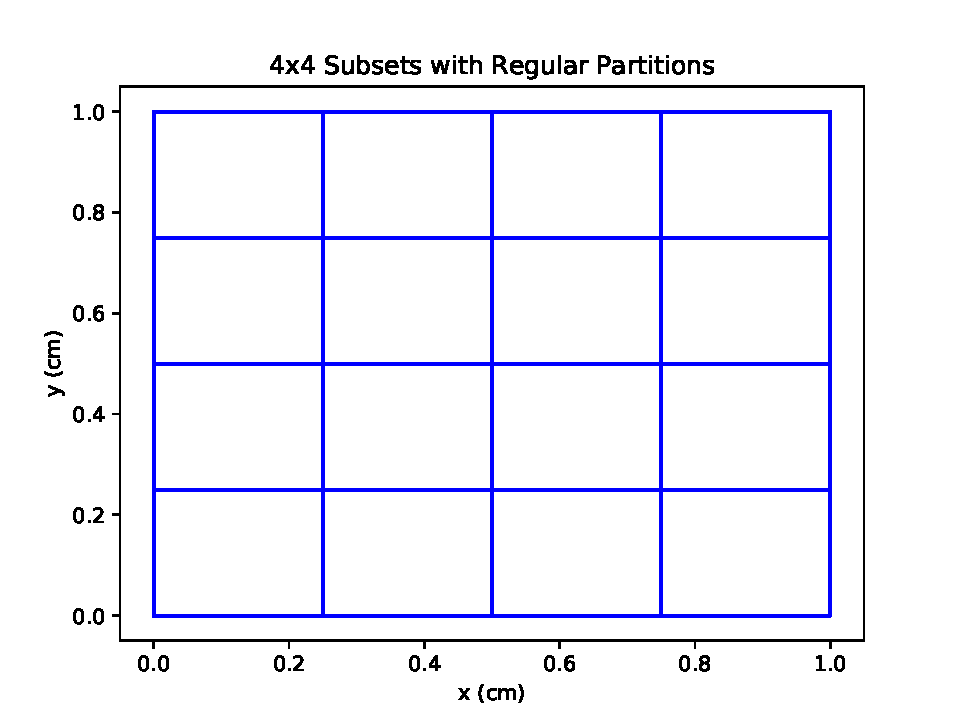
\includegraphics[width=\textwidth]{../Dissertation/cut_line_files/4_regular.pdf}
  \caption{4x4 subsets with regular partitions.}
  \label{4regular}
\end{subfigure}
\begin{subfigure}[b]{0.45\textwidth}
  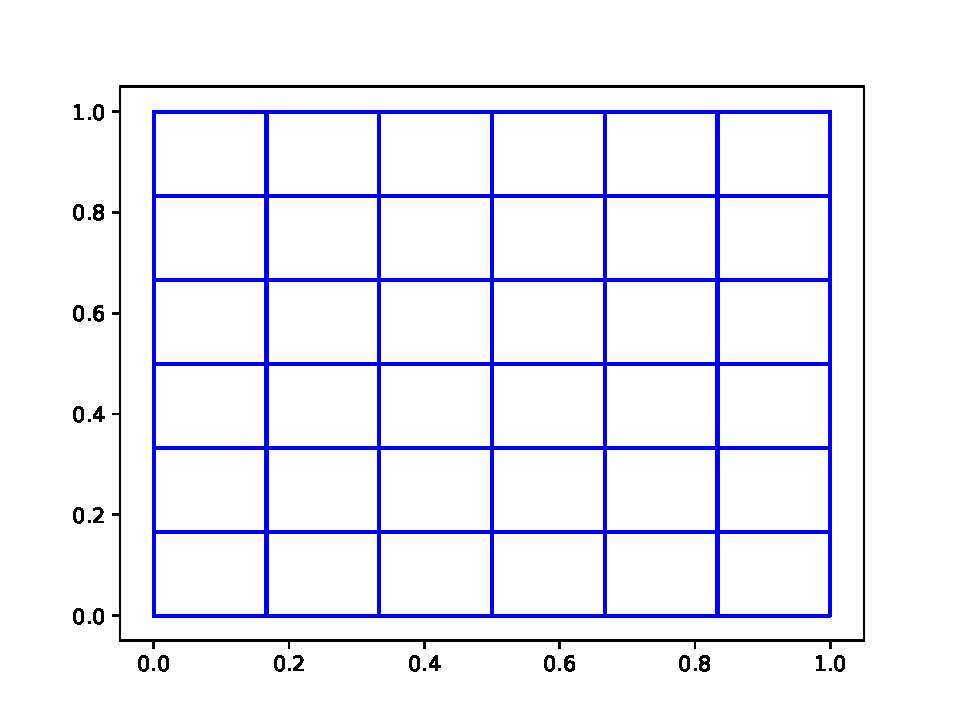
\includegraphics[width=\textwidth]{../Dissertation/cut_line_files/6_regular.pdf}
  \caption{6x6 subsets with regular partitions.}
  \label{6regular}
\end{subfigure}

\begin{subfigure}[b]{0.45\textwidth}
  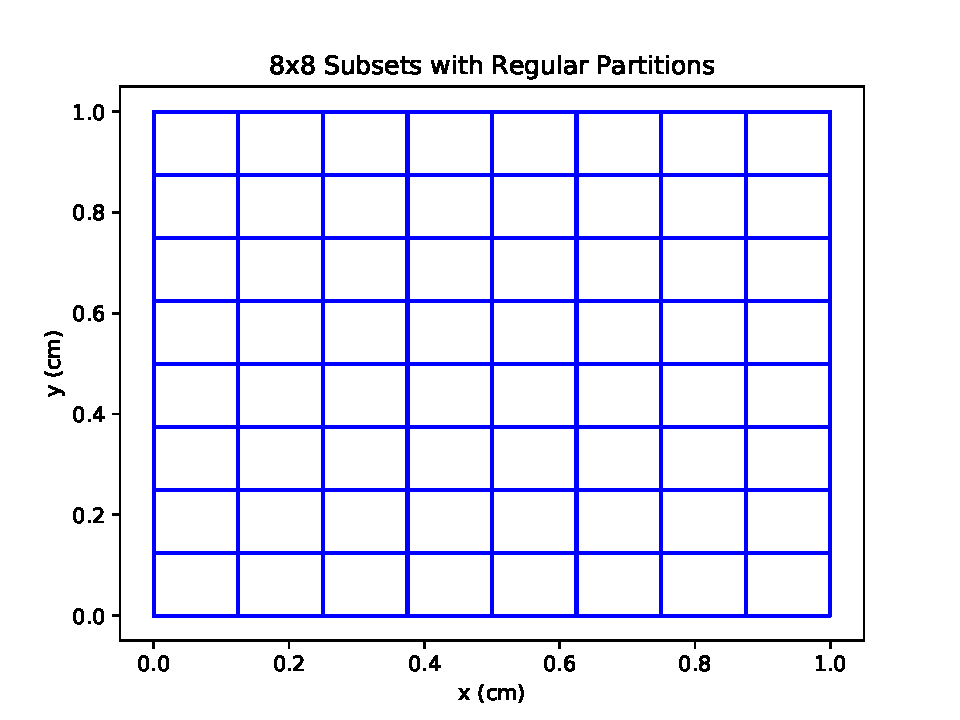
\includegraphics[width=\textwidth]{../Dissertation/cut_line_files/8_regular.pdf}
  \caption{8x8 subsets with regular partitions.}
  \label{8regular}
\end{subfigure}
\begin{subfigure}[b]{0.45\textwidth}
  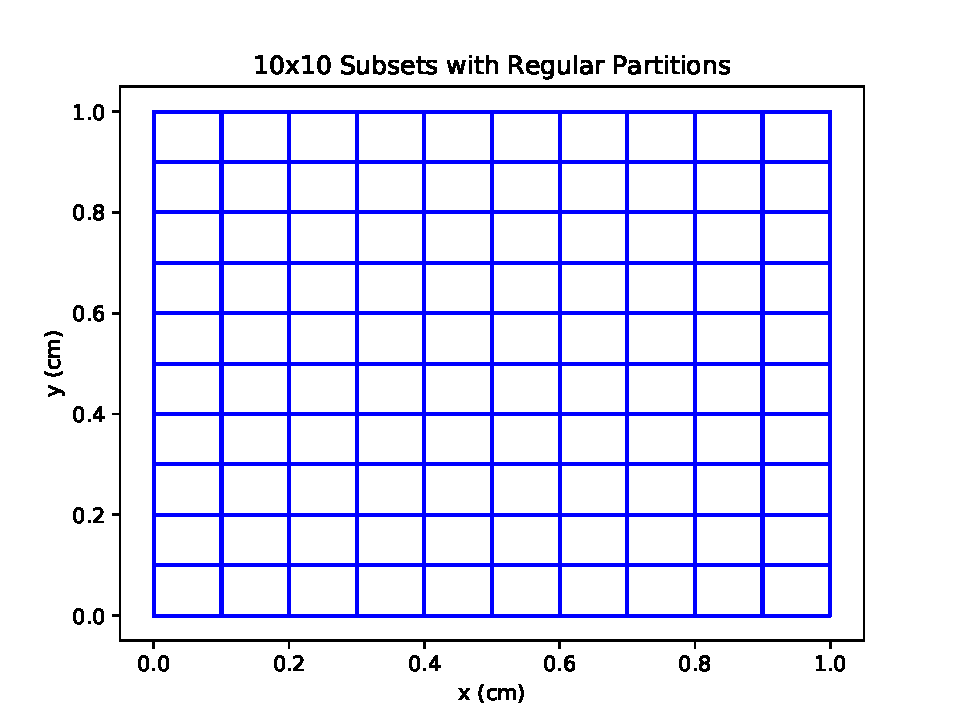
\includegraphics[width=\textwidth]{../Dissertation/cut_line_files/10_regular.pdf}
  \caption{10x10 subsets with regular partitions.}
  \label{10regular}
\end{subfigure}
\caption{Examples of regular partitioning.}
\label{regular_partitions}
\end{figure}

Using regular partitions as shown in Fig.~\ref{regular_partitions}, the first portion of the 2D verification study was run from 2x2 to 10x10 subsets in x and y and 1 to 6 angles per quadrant.  Figure~\ref{regular_verification} shows the results of the time-to-solution estimator (solid line) against Ragusa's code (points) for each test case. The time-to-solution estimator is in perfect agreement for regular partitions with multiple angles per quadrant.

%Verification plots.
\begin{figure}[H]
\centering
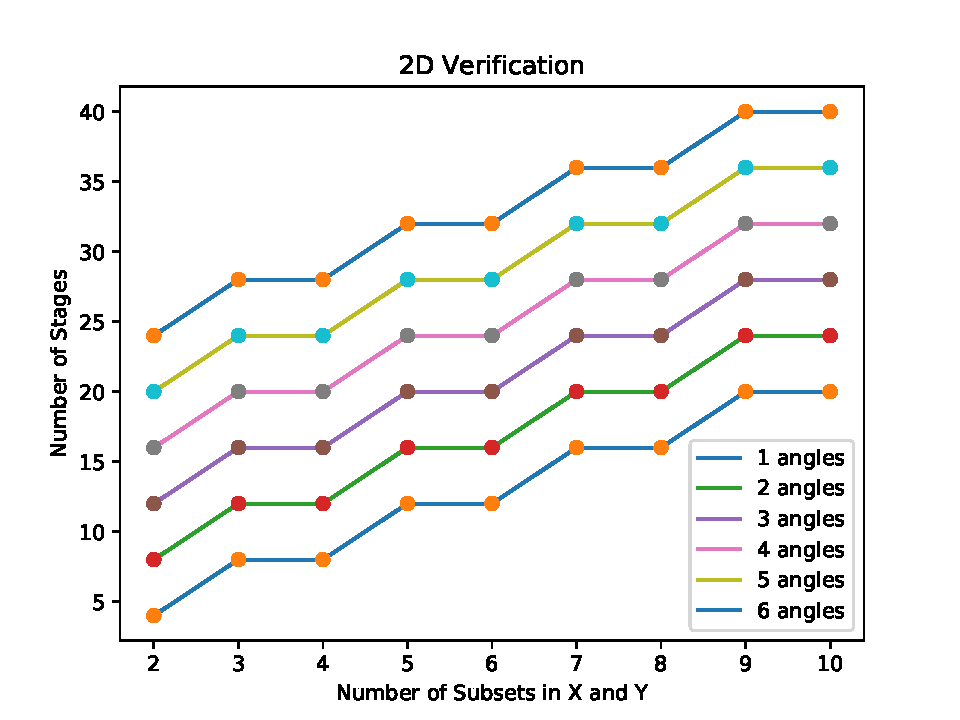
\includegraphics[scale=0.8]{../figures/regular_verification.pdf}
\caption{A 2D verification suite with regular partitions run from 2x2 to 10x10 subsets with each case being run from 1 to 6 anglesets per quadrant.}
\label{regular_verification}
\end{figure}

%%%%%%%%%%%%%%%%%%%%%%%%%%%%%%%%%%%%%%%%%%%%%%%%%%%%%%%%%%%%%%%%%%%%%%%%%%%%%%%%%%%
\subsubsection{``Mildly random'' partitions}
%%%%%%%%%%%%%%%%%%%%%%%%%%%%%%%%%%%%%%%%%%%%%%%%%%%%%%%%%%%%%%%%%%%%%%%%%%%%%%%%%%%
Figure~\ref{mild_random_partitions} shows four examples of the ``mildly random'' partitioning scheme used for the second part of the verification study. Cut lines in the x dimension go all the way across the domain, and are uniformly distributed. This reflects a possible partitioning scheme after the load balancing by dimension algorithm described in Section \ref{sec:lbd} is used.

%Mild random partitions
\begin{figure}[H]
\centering
\begin{subfigure}[b]{0.45\textwidth}
  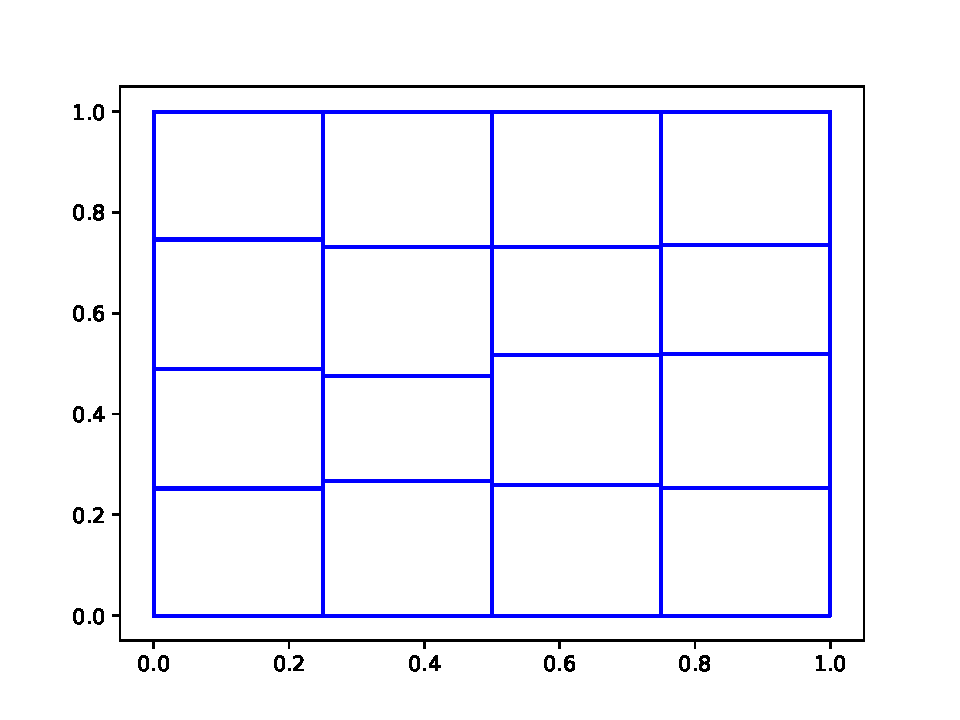
\includegraphics[width=\textwidth]{../Dissertation/cut_line_files/4_mild_random.pdf}
  \caption{4x4 subsets with ``mildly random'' partitions.}
  \label{4mildrandom}
\end{subfigure}
\begin{subfigure}[b]{0.45\textwidth}
  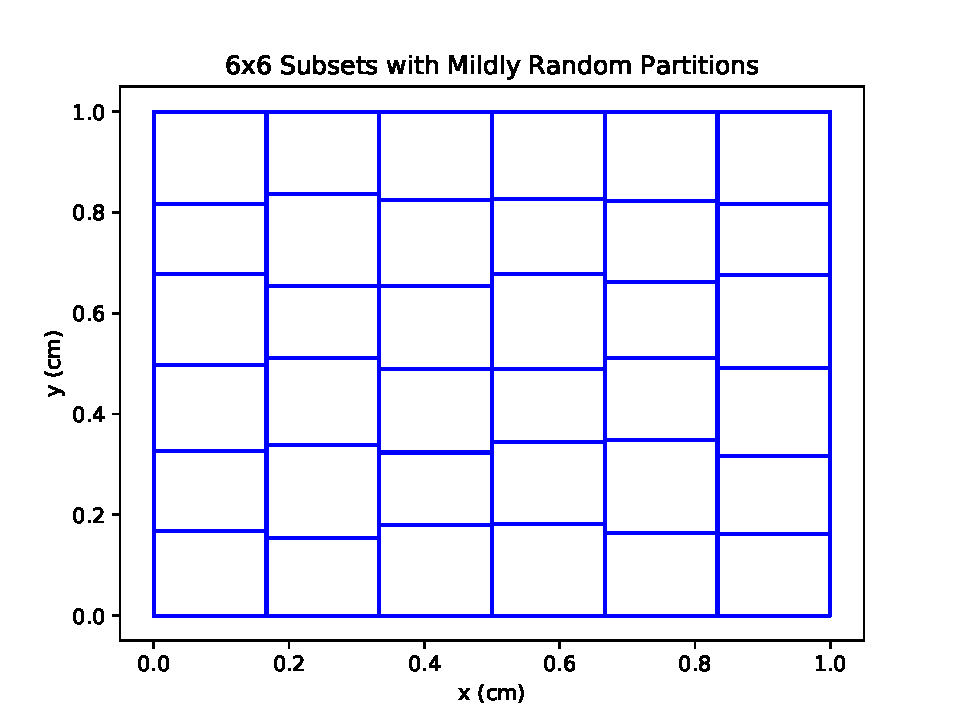
\includegraphics[width=\textwidth]{../Dissertation/cut_line_files/6_mild_random.pdf}
  \caption{6x6 subsets with ``mildly random'' partitions.}
  \label{6mildrandom}
\end{subfigure}

\begin{subfigure}[b]{0.45\textwidth}
  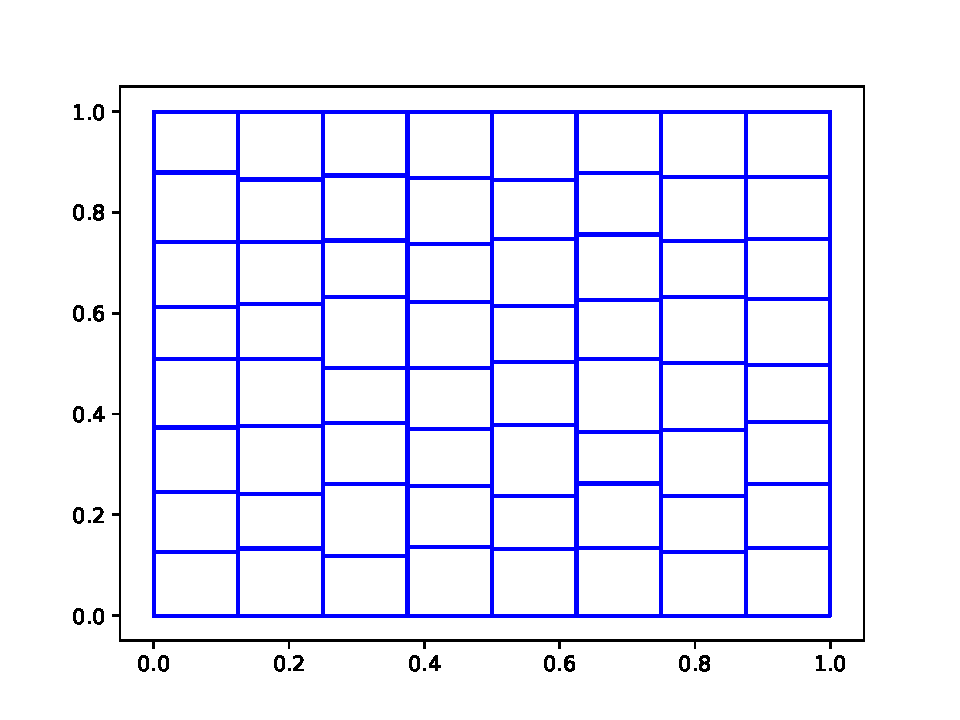
\includegraphics[width=\textwidth]{../Dissertation/cut_line_files/8_mild_random.pdf}
  \caption{8x8 subsets with ``mildly random'' partitions.}
  \label{8mildrandom}
\end{subfigure}
\begin{subfigure}[b]{0.45\textwidth}
  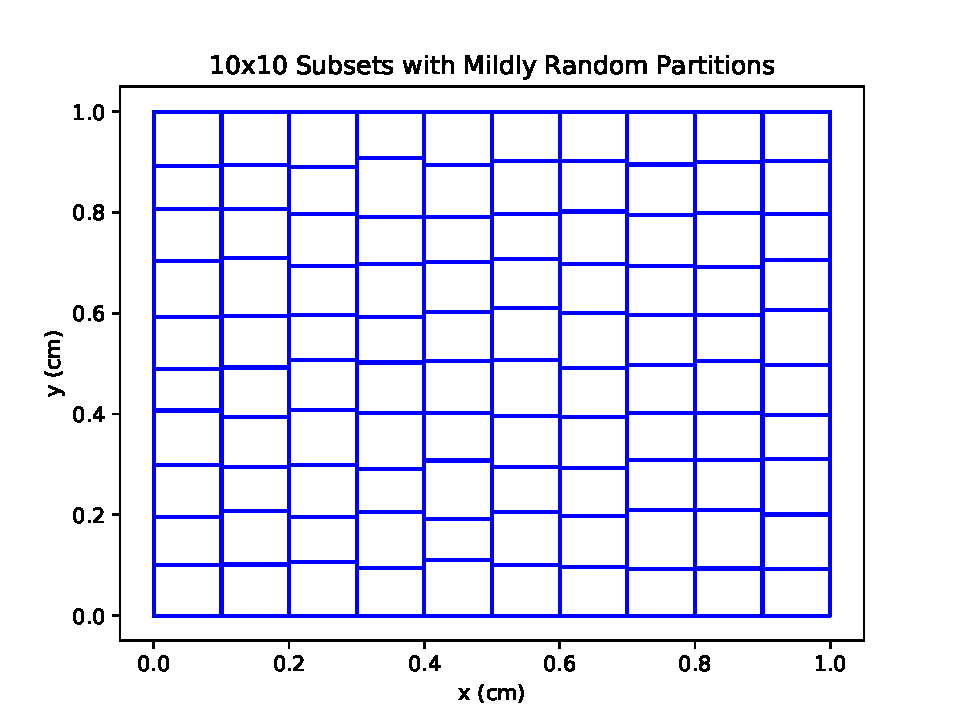
\includegraphics[width=\textwidth]{../Dissertation/cut_line_files/10_mild_random.pdf}
  \caption{10x10 subsets with ``mildly random'' partitions.}
  \label{10mildrandom}
\end{subfigure}
\caption{Examples of ``mildly random'' partitioning.}
\label{mild_random_partitions}
\end{figure}

Using``mildly random'' partitions as shown in Fig.~\ref{mild_random_partitions}, the second portion of the 2D verification study was run from 2x2 to 10x10 subsets in x and y and 1 to 6 angles per quadrant.  Figure~\ref{mild_random_verification} shows the results of the time-to-solution estimator (solid line) against Ragusa's code (points) for each test case. The time-to-solution estimator is in perfect agreement for``mildly random'' partitions with multiple angles per quadrant.

\begin{figure}[H]
\centering
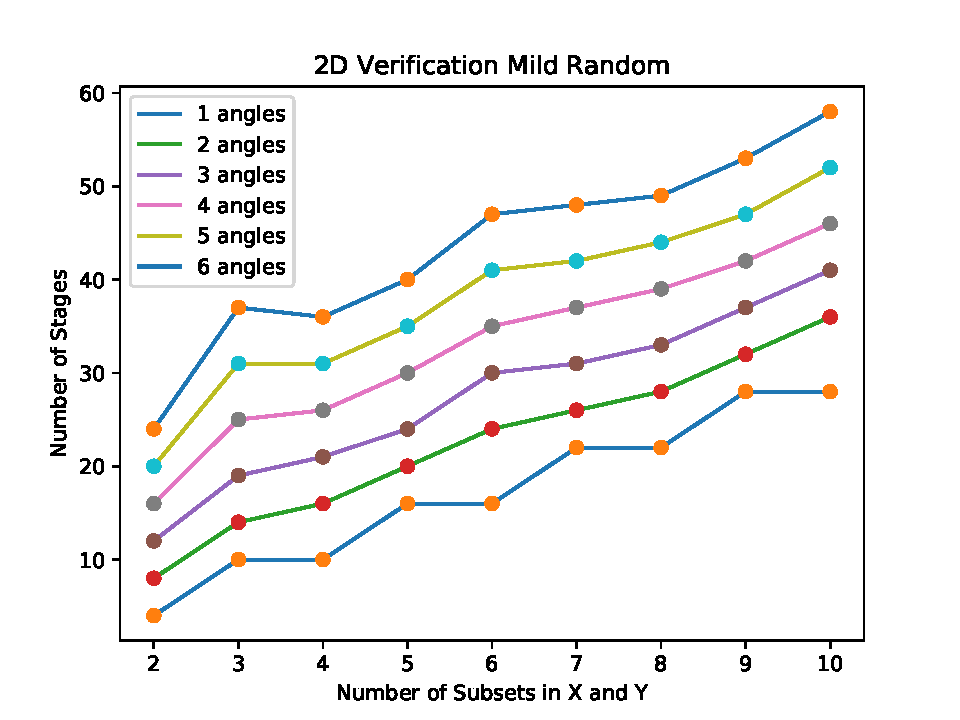
\includegraphics[scale=0.8]{../figures/mild_random_verification.pdf}
\caption{A 2D verification suite with ``mildly random'' partitions run from 2x2 to 10x10 subsets with each case being run from 1 to 6 anglesets per quadrant.}
\label{mild_random_verification}
\end{figure}

%%%%%%%%%%%%%%%%%%%%%%%%%%%%%%%%%%%%%%%%%%%%%%%%%%%%%%%%%%%%%%%%%%%%%%%%%%%%%%%%%%%
\subsubsection{Random partitions}
%%%%%%%%%%%%%%%%%%%%%%%%%%%%%%%%%%%%%%%%%%%%%%%%%%%%%%%%%%%%%%%%%%%%%%%%%%%%%%%%%%%
%Random partitions
Figure~\ref{random_partitions} shows four examples of the ``random'' partitioning scheme used for the third part of the verification study. Cut lines in the x dimension go all the way across the domain, but are not necessarily uniformly distributed. The cut lines in y are randomly distributed in each column.This reflects a possible partitioning scheme after the load balancing by dimension algorithm described in Section \ref{sec:lbd} is used.
\begin{figure}[H]
\centering
\begin{subfigure}[b]{0.45\textwidth}
  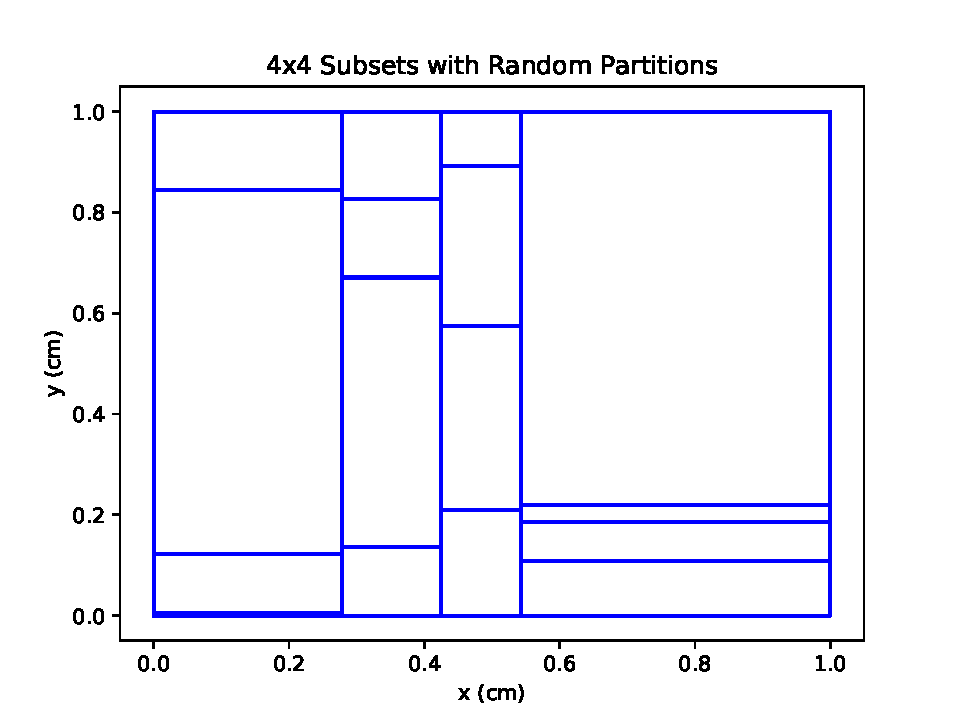
\includegraphics[width=\textwidth]{../Dissertation/cut_line_files/4_random.pdf}
  \caption{4x4 subsets with ``random'' partitions.}
  \label{4random}
\end{subfigure}
\begin{subfigure}[b]{0.45\textwidth}
  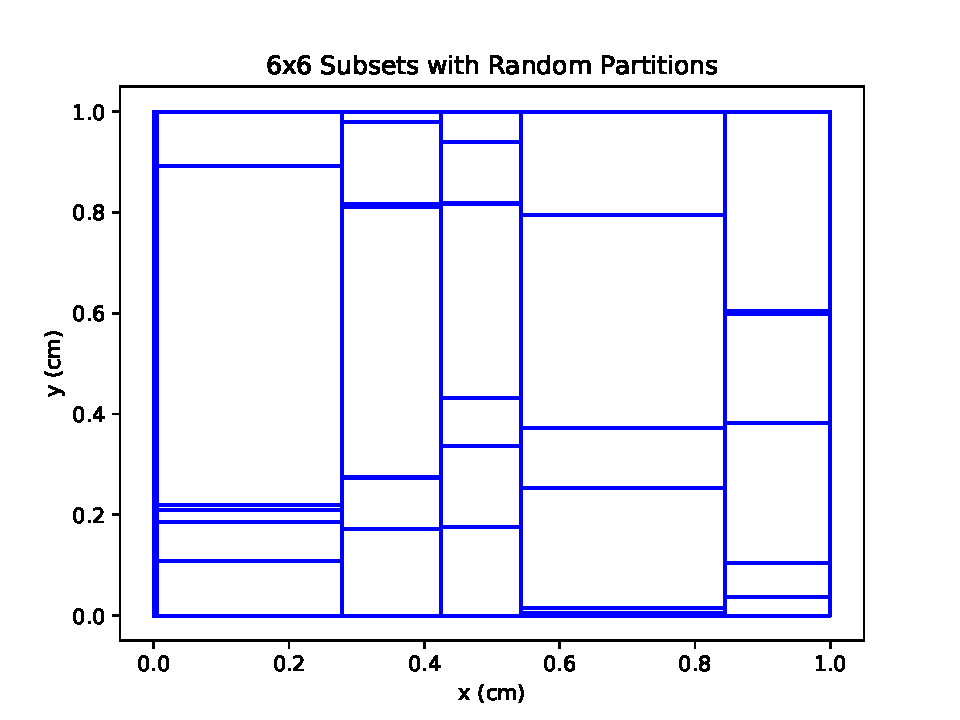
\includegraphics[width=\textwidth]{../Dissertation/cut_line_files/6_random.pdf}
  \caption{6x6 subsets with ``random'' partitions.}
  \label{6random}
\end{subfigure}

\begin{subfigure}[b]{0.45\textwidth}
  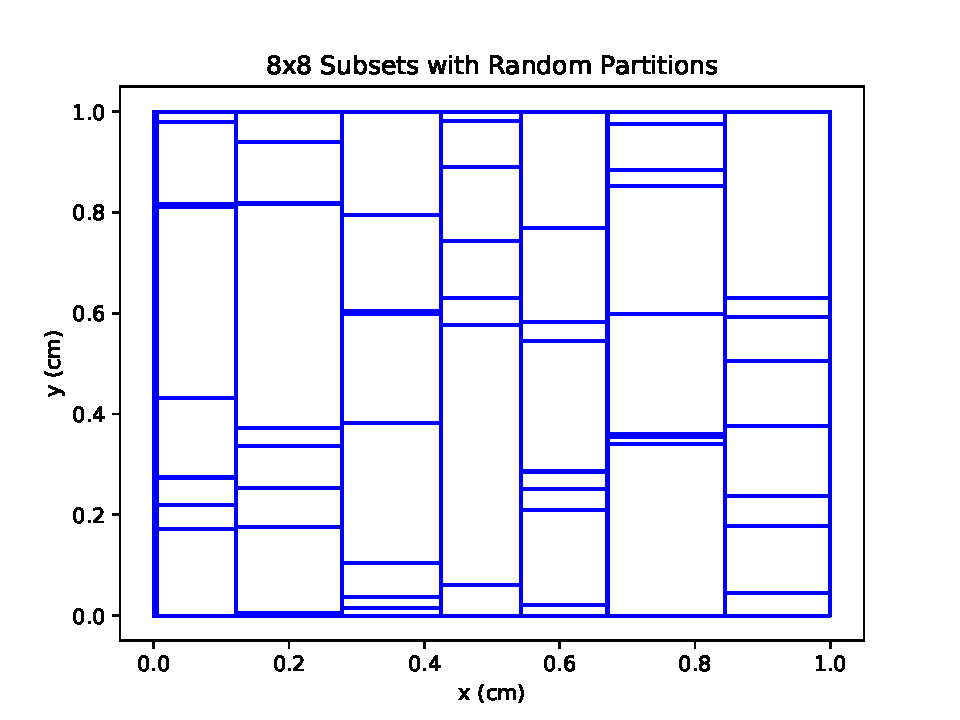
\includegraphics[width=\textwidth]{../Dissertation/cut_line_files/8_random.pdf}
  \caption{8x8 subsets with ``random'' partitions.}
  \label{8random}
\end{subfigure}
\begin{subfigure}[b]{0.45\textwidth}
  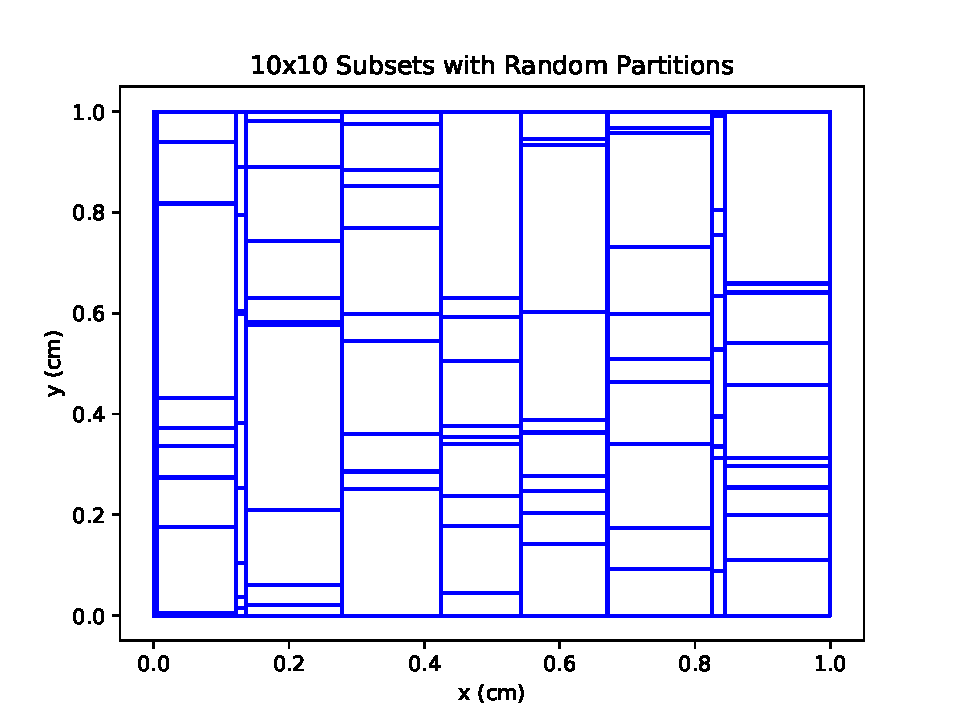
\includegraphics[width=\textwidth]{../Dissertation/cut_line_files/10_random.pdf}
  \caption{10x10 subsets with ``random''partitions.}
  \label{10random}
\end{subfigure}
\caption{Examples of ``random'' partitioning.}
\label{random_partitions}
\end{figure}

Using ``random'' partitions as shown in Fig.~\ref{random_partitions}, the third portion of the 2D verification study was run from 2x2 to 10x10 subsets in x and y and 1 to 6 angles per quadrant.  Figure~\ref{random_verification} shows the results of the time-to-solution estimator (solid line) against Ragusa's code (points) for each test case. The time-to-solution estimator is in perfect agreement for``random''partitions with multiple angles per quadrant.

\begin{figure}[H]
\centering
\includegraphics[scale=0.8]{../figures/random_verification.pdf}
\caption{A 2D verification suite with ``random'' partitions run from 2x2 to 10x10 subsets with each case being run from 1 to 6 anglesets per quadrant.}
\label{random_verification}
\end{figure}

%%%%%%%%%%%%%%%%%%%%%%%%%%%%%%%%%%%%%%%%%%%%%%%%%%%%%%%%%%%%%%%%%%%%%%%%%%%%%%%%%%%
\subsubsection{Probable worst-case partitions}
%%%%%%%%%%%%%%%%%%%%%%%%%%%%%%%%%%%%%%%%%%%%%%%%%%%%%%%%%%%%%%%%%%%%%%%%%%%%%%%%%%%
Figure~\ref{worst_partitions} shows four examples of the probable worst-case partitioning scheme used for the final part of the verification study. Cut lines in the x dimension go all the way across the domain, and are uniformly distributed. The cut lines in y are distributed on opposing ends of alternating columns.This reflects a possible partitioning scheme after the load balancing by dimension algorithm described in Section \ref{sec:lbd} is used.
\begin{figure}[H]
\centering
\begin{subfigure}[b]{0.45\textwidth}
  \includegraphics[width=\textwidth]{../Dissertation/cut_line_files/4_worst.pdf}
  \caption{4x4 subsets with probable worst-case partitions.}
  \label{4worst}
\end{subfigure}
\begin{subfigure}[b]{0.45\textwidth}
  \includegraphics[width=\textwidth]{../Dissertation/cut_line_files/6_worst.pdf}
  \caption{6x6 subsets with probable worst-case partitions.}
  \label{6worst}
\end{subfigure}

\begin{subfigure}[b]{0.45\textwidth}
  \includegraphics[width=\textwidth]{../Dissertation/cut_line_files/8_worst.pdf}
  \caption{8x8 subsets with probable worst-case partitions.}
  \label{8random}
\end{subfigure}
\begin{subfigure}[b]{0.45\textwidth}
  \includegraphics[width=\textwidth]{../Dissertation/cut_line_files/10_worst.pdf}
  \caption{10x10 subsets with probable worst-case partitions.}
  \label{10random}
\end{subfigure}
\caption{Examples of probable worst-case partitioning.}
\label{worst_partitions}
\end{figure}
Using probable worst-case partitions as shown in Fig.~\ref{worst_partitions}, the final portion of the 2D verification study was run from 2x2 to 10x10 subsets in x and y and 1 to 6 angles per quadrant.  Figure~\ref{worst_verification} shows the results of the time-to-solution estimator (solid line) against Ragusa's code (points) for each test case. The time-to-solution estimator is in perfect agreement for probable worst-case partitions with multiple angles per quadrant.
\begin{figure}[H]
\centering
\includegraphics[scale=0.8]{../figures/worst_verification.pdf}
\caption{A 2D verification suite with probable worst-case partitions run from 2x2 to 10x10 subsets with each case being run from 1 to 6 angles per quadrant.}
\label{worst_verification}
\end{figure}

%%%%%%%%%%%%%%%%%%%%%%%%%%%%%%%%%%%%%%%%%%%%%%%%%%%%%%%%%%%%%%%%%%%%%%%%%%%%%%%%%%%
\subsection{3D Verification}
%%%%%%%%%%%%%%%%%%%%%%%%%%%%%%%%%%%%%%%%%%%%%%%%%%%%%%%%%%%%%%%%%%%%%%%%%%%%%%%%%%%
PDT's performance model is used to verify stage counts for 3D problems with regular grids.
Figure~\ref{3d_verification} shows PDT's performance model stage counts are in perfect agreement with the time-to-solution estimator's stage counts for 2\textsuperscript{3} to 10\textsuperscript{3} subsets and from 1 to 6 angles per octant.

\begin{figure}[H]
\centering
\includegraphics[scale=0.8]{../figures/3d_verification.pdf}
\caption{A 3D verification suite with regular partitions run from 2\textsuperscript{3} to 10\textsuperscript{3} subsets with each case being run from 1 to 6 angles per octant.}
\label{3d_verification}
\end{figure}


%%%%%%%%%%%%%%%%%%%%%%%%%%%%%%%%%%%%%%%%%%%%%%%%%%%%%%%%%%%%%%%%%%%%%%%%%%%%%%%%%%%
\subsection{PDT's Performance Model vs. Time-to-Solution Estimator}
%%%%%%%%%%%%%%%%%%%%%%%%%%%%%%%%%%%%%%%%%%%%%%%%%%%%%%%%%%%%%%%%%%%%%%%%%%%%%%%%%%%

PDT has run a scaling suite out to 90,112 cores on the Quartz supercomputer \cite{quartz} at Lawrence Livermore National Lab (LLNL).
A smaller scaling suite, tabulated in Table \ref{scaling_suite} is the first benchmark case run for the time-to-solution estimator.
The suite was run with 1 energy group, 80 directions, $A_m = 10$, $A_x=\frac{N_x}{P_x}$, $A_y=\frac{N_y}{P_y}$, and $A_z = 1$.
The following machine parameters were generated and used for the 1 group suite:
\begin{itemize}
  \item $T_c = 2683.769$ ns
  \item $T_m = 111.972$ ns
  \item $T_g = 559.127$ ns
  \item $T_\text{byte} = 4.47$ ns
  \item $\text{latency }= 4110$ ns
  \item $M_L = 2.5$
  \item $T_{wu} = 5779.929$ ns
  \item mcff = 1.32
\end{itemize}

\begin{table}[H]
  \centering
  \caption{The scaling suite parameters ran with 1 energy group, 80 directions, and $A_m = 10$.}
  \label{scaling_suite}
  \begin{tabular}{c|c|c|c|c|c|c|c|c|c}
    \textbf{Cores} & 1 & 8 & 64 & 512 & 1,204 & 2,048 & 4,096 & 8,192 & 16,384 \\ \hline
    \textbf{Nx} & 16 & 32 & 64 & 128 & 128 & 256 & 256 & 256 & 512 \\ \hline
    \textbf{Ny} & 16 & 32 & 64 & 128 & 128 & 128 & 128 & 256 & 256 \\ \hline
    \textbf{Nz} & 16 & 32 & 64 & 128 & 256 & 256 & 256 & 512 & 512 \\ \hline
    \textbf{Px} & 1  & 2  & 8  & 16  & 32  & 32  & 64  & 64  & 128 \\ \hline
    \textbf{Py} & 1  & 2  & 4  & 16  & 16  & 32  & 32  & 64  & 64  \\ \hline
    \textbf{Pz} & 1  & 2  & 2  & 2   & 2   & 2   & 2   & 2   & 2   \\
  \end{tabular}
\end{table}

Figure~\ref{scaling_stagecount} shows the stage counts of the scaling suite for PDT's performance model and the time-to-solution estimator are in perfect agreement.
Figures \ref{weak_scaling_tts_sweep} and \ref{weak_scaling_tts} show the time per sweep and parallel efficiency for (1) PDT, (2) the PDT performance model, and (3) the time-to-solution estimator. Table \ref{scaling_percent_diff} tabulates the percent differences for (1) PDT and the performance model, (2) the performance model, and (3) the time-to-solution estimator, and PDT and the time-to-solution estimator.

It is notable that the time-to-solution estimator consistently returns a smaller sweep time value than PDT's performance model. This is certainly in part due to the assumption from PDT's performance model that each processors at each stage communicate to the same amount of neighbors (three neighbors in 3D, 2 in 2D).
In reality, this is not the case, as processors in the corners of the domain will communicate to fewer neighbors for certain directions, and the final processor for a direction does not communicate to any neighbors (as it has no successors).
Because the stage counts for the performance model and time-to-solution estimator are in perfect agreement (as shown in Fig.~\ref{scaling_stagecount}), we know that this slight overestimation of the performance model is a reason for its consistently higher sweep times.
Even given these differences, the time-to-solution estimator is consistently within 4\% of the performance model, as tabulated in Table \ref{scaling_percent_diff}.

The performance model's slightly better accuracy in predicting PDT's sweep time is likely due to processor noise and slight variations in latency on Quartz driving up PDT's sweep time. This masks the performance model's slight overestimation of the sweep time.

Figure~\ref{weak_scaling_tts} shows PDT's performance model and the time-to-solution estimator scale with near equivalence. The model and the time-to-solution estimator predict PDT's scaling well, although there are slight differences that can be attributed to the differences in sweep times tabulated in Table \ref{scaling_percent_diff}.
\begin{figure}[ht]
\centering
\includegraphics[scale=0.8]{../figures/scaling_stagecount.pdf}
\caption{The stage counts of PDT's performance model and the time-to-solution estimator for the scaling suite in Table \ref{scaling_suite}.}
\label{scaling_stagecount}
\end{figure}
\begin{figure}[ht]
\centering
\includegraphics[scale=0.8]{../figures/scaling_tts_sweep_times.pdf}
\caption{The time per sweep of PDT, the PDT performance model, and the time-to-solution estimator.}
\label{weak_scaling_tts_sweep}
\end{figure}
\begin{figure}[ht]
\centering
\includegraphics[scale=0.8]{../figures/scaling_tts.pdf}
\caption{The parallel efficiency relative to 8 cores of PDT, the PDT performance model, and the time-to-solution estimator.}
\label{weak_scaling_tts}
\end{figure}
\begin{table}[ht]
\centering
\caption{The percent difference between (1) PDT and its performance model, (2) PDT's performance model and the time-to-solution estimator, and (3) PDT and the time-to-solution estimator.}
\label{scaling_percent_diff}
\begin{tabular}{c|c|c|c}
\textbf{Cores} & \textbf{PDT v. Perf.} & \textbf{Perf. v. TTS} & \textbf{PDT v. TTS} \\ \hline
1&8.82\%&0.68\%&9.44\% \\ \hline
8&6.67\%&1.86\%&8.4\% \\ \hline
64&2.22\%&2.04\%&4.22\% \\ \hline
512&8.0\%&1.52\%&9.4\% \\ \hline
1024&2.0\%&3.67\%&5.6\% \\ \hline
2048&2.0\%&2.21\%&4.17\% \\ \hline
4096&3.77\%&3.24\%&6.89\% \\ \hline
8192&8.33\%&3.8\%&11.82\% \\ \hline
16384&9.68\%&2.7\%&12.11\%
\end{tabular}
\end{table}

%%%%%%%%%%%%%%%%%%%%%%%%%%%%%%%%%%%%%%%%%%%%%%%%%%%%%%%%%%%%%%%%%%%%%%%%%%%%%%%%%%%
\subsection{PDT vs. Time-to-Solution Estimator for Unstructured Meshes}
%%%%%%%%%%%%%%%%%%%%%%%%%%%%%%%%%%%%%%%%%%%%%%%%%%%%%%%%%%%%%%%%%%%%%%%%%%%%%%%%%%%

The motivation to develop the time-to-solution estimator was born out of the desire to predict sweep time for unstructured meshes.
To test how the time-to-solution estimator performs on unstructured problems, we use the meshes from our load balancing parametric study: the unbalanced pin mesh(Fig. \ref{partitioning_example}) and the Level-2 experiment mesh (Fig. \ref{level2_nocut_lbchapter}).

All problems were run with one energy group, one subset per processor, and 144 angles with $A_m = 36$, or 36 angles per angleset. The machine parameters used for all problems are:
\begin{itemize}
  \item $T_c = 1208.383$ ns
  \item $T_m = 65.54614$ ns
  \item $T_g = 175.0272$ ns
  \item $T_\text{byte} = 4.47$ ns
  \item $\text{latency }= 4110$ ns
  \item $T_{wu} = 147.0754$ ns
  \item mcff = 1.181
\end{itemize}

For each result presented, the problem is run through PDT 10 times on the Quartz supercomputer.
This allows us to filter out outlying values due to supercomputer noise by taking the median solve time per sweep for each problem.
For each result in PDT, the median sweep time value, the maximum sweep time value, and the minimum sweep time value are plotted to showcase the outlying values that can occur.
In order to minimize the effects of the sweep overhead on the timing statistics, the solve time per sweep is calculated from the mean time of ten transport sweeps for each case.

%%%%%%%%%%%%%%%%%%%%%%%%%%%%%%%%%%%%%%%%%%%%%%%%%%%%%%%%%%%%%%%%%%%%%%%%%%%%%%%%%%%
\subsubsection{PDT vs. the time-to-solution estimator for the unbalanced pin mesh}
%%%%%%%%%%%%%%%%%%%%%%%%%%%%%%%%%%%%%%%%%%%%%%%%%%%%%%%%%%%%%%%%%%%%%%%%%%%%%%%%%%%

Figure~\ref{comp_reg_spiderweb} shows the sweep times for PDT and the time-to-solution estimator for the unbalanced pin mesh with 2 to 10 subsets in each dimension with regular cuts.
Table \ref{diff_reg_spiderweb} tabulates the percent difference between PDT and the time-to-solution estimator for each of the regular test cases run.
We notice that there is better agreement for cases where there are more unknowns.
These cases for the the unbalanced pin mesh with regular cuts are cases with 3, 4, 6, 7, 8, and 9 subsets in each dimension, with cut lines cutting through cells and increasing the total number of cells throughout the mesh.
Cases with 2, 5, and 10 subsets in each dimension have cuts coinciding with natural boundaries, adding no unknowns to the mesh.
More unknowns lead to better timing statistics for PDT, increasing the likelihood of agreement with the time-to-solution estimator.
%spiderweb comp for reg
\begin{figure}[!ht]
\centering
\includegraphics[scale=0.75]{../figures/spiderweb_reg_pdtvtts.pdf}
\caption{The sweep times of the time-to-solution estimator and PDT for the unbalanced pin mesh for 2 to 10 subsets in each dimension with regular cuts.}
\label{comp_reg_spiderweb}
\end{figure}
\begin{table}[!ht]
\centering
\caption{The percent difference in sweep times between the time-to-solution estimator and PDT for the sweep times shown in Fig.~\ref{comp_reg_spiderweb}.}
\label{diff_reg_spiderweb}
\begin{tabular}{c|c}
\textbf{$\sqrt{\text{Num Subsets}}$} & \bf PDT vs. TTS \\ \hline
2&19.93\%\\ \hline
3&12.3\%\\ \hline
4&1.75\%\\ \hline
5&15.69\%\\ \hline
6&2.71\%\\ \hline
7&2.61\%\\ \hline
8&4.45\%\\ \hline
9&3.21\%\\ \hline
10&11.38\%
\end{tabular}
\end{table}

Figure~\ref{comp_lb_spiderweb} shows the sweep times for PDT and the time-to-solution estimator for 2 to 10 subsets in each dimension with load-balanced cuts.
If we focus on the maximum PDT sweep time in the 5 subset case in Fig.~\ref{comp_lb_spiderweb}, we can see that PDT can sometimes produce outliers during runs.
For that reason, we take the median, not the mean, sweep time value from the ten PDT runs to get the best representation of PDT's solve time per sweep.
Table \ref{diff_lb_spiderweb} tabulates the percent difference between PDT and the time-to-solution estimator for each case run.
We notice that we have poorer agreement with load-balanced cuts than with regular cuts, particularly for lower subset cases.
This is possibly due to the first-come-first scheduler in PDT and the schedule of the time-to-solution estimator schedule not being in perfect agreement.
While the time-to-solution estimator's schedule is deterministic, there are no guarantees that PDT's first-come-first-serve schedule is repeatable or that it matches the time-to-solution estimator.
If there are two tasks that have a similar amount of unknowns, the processor with more unknowns may solve and communicate them faster than the processor with less unknowns.
This would cause a disagreement between the time-to-solution estimator and PDT.
The low subset cases happen to be the more balanced cases for the unbalanced pin mesh with load-balanced cuts.
The 2, 3, and 4 subset cases for the unbalanced pin mesh have load-balance metric values of $f = 1.76, 2.58,$ and $2.38$ respectively.
With a more even distribution of cells, PDT's first-come-first-serve schedule is likelier to deviate more as certain processors may be faster than their neighboring processors.
%spiderweb comp for lb
\begin{figure}[!ht]
  \centering
  \includegraphics[scale=0.75]{../figures/spiderweb_lb_pdtvtts.pdf}
  \caption{The sweep times of the time-to-solution estimator and PDT for the mesh in Fig.~\ref{partitioning_example} for 2 to 10 subsets in each dimension with load-balanced cuts.}
\label{comp_lb_spiderweb}
\end{figure}
\begin{table}[!ht]
\centering
\caption{The percent difference in sweep times between the time-to-solution estimator and PDT for the sweep times shown in Fig.~\ref{comp_lb_spiderweb}.}
\label{diff_lb_spiderweb}
\begin{tabular}{c|c}
\textbf{$\sqrt{\text{Num Subsets}}$} & \bf PDT vs. TTS \\ \hline
2&15.9\%\\ \hline
3&23.52\%\\ \hline
4&41.83\%\\ \hline
5&6.15\%\\ \hline
6&10.67\%\\ \hline
7&8.43\%\\ \hline
9&15.47\%\\ \hline
10&7.88\%
\end{tabular}
\end{table}

Figure~\ref{comp_lbd_spiderweb} shows the sweep times for PDT and the time-to-solution estimator for 2 to 10 subsets in each dimension with load-balanced-by-dimension cuts.
Table \ref{diff_lbd_spiderweb} tabulates the percent difference between PDT and the time-to-solution estimator for each case run.
The load-balanced-by-dimension cases for the unbalanced pin mesh have more consistent agreement than the regular cut and load-balanced cut cases.
With load balancing by dimension, more cells are consistently created by slicing through cells in order to get more balanced partitions.
By increasing the number of unknowns, we get better timing statistics for the solve time per sweep.
In addition, with load-balanced-by-dimension partitions, PDT's first-come-first-serve scheduler is more likely to agree with the time-to-solution estimator's.
The communication dependencies inherently created by load-balanced-by-dimension partitions mitigate the likelihood of faster processors disrupting the expected schedule, as seen with the load-balanced cases.
%%%spiderweb comp for lbd
\begin{figure}[!ht]
  \centering
  \includegraphics[scale=0.75]{../figures/spiderweb_lbd_pdtvtts.pdf}
  \caption{The sweep times of the time-to-solution estimator and PDT for the mesh in Fig.~\ref{partitioning_example} for 2 to 10 subsets in each dimension with load-balanced-by-dimension cuts.}
\label{comp_lbd_spiderweb}
\end{figure}
\begin{table}[!ht]
\centering
\caption{The percent difference in sweep times between the time-to-solution estimator and PDT for the sweep times shown in Fig.~\ref{comp_lbd_spiderweb}.}
\label{diff_lbd_spiderweb}
\begin{tabular}{c|c}
\textbf{$\sqrt{\text{Num Subsets}}$} & \bf PDT vs. TTS \\ \hline
2&6.5\%\\ \hline
3&13.49\%\\ \hline
4&4.04\%\\ \hline
6&2.78\%\\ \hline
7&3.5\%\\ \hline
9&4.18\%\\ \hline
10&12.01\%
\end{tabular}
\end{table}

\FloatBarrier
Figure~\ref{ubp_more_sparse} shows a more refined version of the unbalanced pin mesh, containing 9656 cells as opposed to 420 cells. 
Figure~\ref{comp_reg_sparse} shows the sweep times for PDT and the time-to-solution estimator for the unbalanced pin mesh with 2 to 10 subsets in each dimension with regular cuts.
Table \ref{diff_reg_sparse} tabulates the percent difference between PDT and the time-to-solution estimator for each of the regular test cases run.
%%%%
\begin{figure}[H]
\centering
\includegraphics[scale=0.28]{../figures/unbalanced_pins_more_sparse.png}
\caption{A more refined version of the unbalanced pin mesh, containing 9656 cells as opposed to 420 cells.}
\label{ubp_more_sparse}
\end{figure}
%%%
\begin{figure}[h]
\centering
\includegraphics{../figures/more_sparse_reg_pdtvtts.pdf}
\caption{The sweep times of the time-to-solution estimator and PDT for the more refined unbalanced pin mesh for 2 to 10 subsets in each dimension with regular cuts}
\label{comp_reg_sparse}
\end{figure}
%%%
\begin{table}[h]
\centering
\caption{The percent difference in sweep times between the time-to-solution estimator and PDT for the sweep times shown in Fig.~\ref{comp_reg_sparse}.}
\label{diff_reg_sparse}
\begin{tabular}{c|c}
\textbf{$\sqrt{\text{Num Subsets}}$} & \bf PDT vs. TTS \\ \hline 
2&21.14\%\\ \hline 
3&15.87\%\\ \hline 
4&10.96\%\\ \hline 
5&9.3\%\\ \hline 
6&1.47\%\\ \hline 
7&0.41\%\\ \hline 
8&3.68\%\\ \hline 
9&2.85\%\\ \hline 
10&6.62\%
\end{tabular}
\end{table}

The 9656 cell unbalanced pin mesh time-to-solution estimator sweep times show more consistent agreement with PDT than the 420 cell unbalanced pin mesh.
In addition, the behaviors of PDT and the time-to-solution estimator are more consistent with each other with more cells.
The low core cases disagree once more, likely due to an overestimation of the latency by the time-to-solution estimator.
Properly characterizing the latency for individual core counts is likely to improve agreement at low core counts. 

\FloatBarrier
%%%%%%%%%%%%%%%%%%%%%%%%%%%%%%%%%%%%%%%%%%%%%%%%%%%%%%%%%%%%%%%%%%%%%%%%%%%%%%%%%%%
\subsubsection{PDT vs. the time-to-solution estimator for the Level-2 experiment mesh}
%%%%%%%%%%%%%%%%%%%%%%%%%%%%%%%%%%%%%%%%%%%%%%%%%%%%%%%%%%%%%%%%%%%%%%%%%%%%%%%%%%%
Figures \ref{level2_42x13} and \ref{level2_42x13_balanced} show the mesh for the Level-2 experiment with 42 subsets in $x$, and 13 subsets in $y$ with evenly spaced cut lines and balanced cut lines.
The balanced mesh was ``hand-balanced'' by Marvin Adams, Michael Adams, and Jan Vermaak to achieve better load balancing than the automated load balancing algorithm was able to achieve.
\begin{figure}[H]
\centering
\includegraphics[scale=0.28]{../figures/level2_42x13.png}
\caption{The Level-2 experiment mesh evenly partitioned into 42 subsets in x and 13 subsets in y. $f = 32.616$.}
\label{level2_42x13}
\end{figure}
\begin{figure}[H]
\centering
\includegraphics[scale=0.28]{../figures/level2_42x13_balanced.png}
\caption{The Level-2 experiment mesh partitioned and manually load balanced with 42 subsets in x and 13 subsets in y. $f = 2.386$.}
\label{level2_42x13_balanced}
\end{figure}

Table \ref{level2_sweep_times} shows the sweep times for the regular cut and balanced cut Level-2 problems for PDT and the time-to-solution estimator. The minimum and maximum solve time per sweep values are also tabulated.
Table \ref{level2_percent_diff} shows the percent difference between the PDT sweep time and the time-to-solution estimator sweep time.
\begin{table}[ht]
\centering
\caption{The sweep times for the regular cut and manually balanced cut Level-2 problems for PDT and the time-to-solution estimator.}
\label{level2_sweep_times}
\begin{tabular}{c|c|c|c|c}
\bf Case & \bf PDT (s) & \bf TTS (s) & \bf PDT Min (s) & \bf PDT Max (s) \\ \hline
Regular & 0.07 & 0.0648 & 0.0686 & 0.0889\\ \hline
Manually Balanced & 0.0531 & 0.0535 & 0.0522 & 0.0638
\end{tabular}
\end{table}
\begin{table}[ht]
\centering
\caption{The percent difference for the regular cut and manually balanced cut Level-2 problems between PDT and the time-to-solution estimator.}
\label{level2_percent_diff}
\begin{tabular}{c|c}
\textbf{Case} & \bf PDT vs. TTS \\ \hline
Regular & 7.52\% \\ \hline
Manually Balanced & 0.63\%
\end{tabular}
\end{table}
Both the regular and balanced cases have estimated sweep times within 8\% of PDT's sweep times.
Because both of these problems have between 3,000 and 4,000 cells, the number of unknowns in the problem can mitigate the effects seen in the unbalanced pin cases.
The difference in schedule in addition to latency instabilities at 546 cores are less significant with larger problems.

In the future, the schedule from the time-to-solution estimator should be fed into PDT and see if the agreement improves.
In addition, the latency on a machine like Quartz is easy to mischaracterize.
A supercomputer of that size and in constant use can have differing latencies depending on how many nodes are in use and which particular nodes are in use.
The data generated for the scaling suite was done during dedicated access time, when latencies are much easier to characterize with only one user using the entire machine, explaining the good agreement out to 16,000 cores.

Additionally, the machine parameters were generated empirically using a serial suite of structured mesh problems.
In the future, obtaining machine parameters should be attempted using unstructured meshes, and agreement between PDT and the time-to-solution estimator restudied.

%%%%%%%%%%%%%%%%%%%%%%%%%%%%%%%%%%%%%%%%%%%%%%%%%%%%%%%%%%%%%%%%%%%%%%%%%%%%%%%%%%%
%%%%%%%%%%%%%%%%%%%%%%%%%%%%%%%%%%%%%%%%%%%%%%%%%%%%%%%%%%%%%%%%%%%%%%%%%%%%%%%%%%%
\section{Choosing optimal partitions}\label{cha:optimization}
%%%%%%%%%%%%%%%%%%%%%%%%%%%%%%%%%%%%%%%%%%%%%%%%%%%%%%%%%%%%%%%%%%%%%%%%%%%%%%%%%%%
%%%%%%%%%%%%%%%%%%%%%%%%%%%%%%%%%%%%%%%%%%%%%%%%%%%%%%%%%%%%%%%%%%%%%%%%%%%%%%%%%%%
\tcr{
\begin{enumerate}
\item a short paragraph to introduce the rationale + the subsequent subsections.
\item we need to organize the discourse (logical flow of information we give). I generally like the data but it needs to be shrunk. examples of figures I can live WITHOUT: 49--50.
\item We have 9 pages here. I think 5-7 is better.
\end{enumerate}
}
In Chapter \ref{cha:tts}, we have seen that we can estimate the time-to-solution for a sweep for different partitioning schemes.
We use the time-to-solution estimator as the objective function in two optimization methods.
The first optimization method utilizes scipy's optimize library, and the second method utilizes knowledge of a problem's mesh layout to assist in partition placement.
%%%%%%%%%%%%%%%%%%%%%%%%%%%%

%%%%%%%%%%%%%%%%%%%%%%%%%%%%%%%%%%%%%%%%%%%%%%%%%%%%%%%%%%%%%%%%%%%%%%%%%%%%%%%%%%%
\subsection{Scipy Optimize}
%%%%%%%%%%%%%%%%%%%%%%%%%%%%%%%%%%%%%%%%%%%%%%%%%%%%%%%%%%%%%%%%%%%%%%%%%%%%%%%%%%%
The scipy optimize library \cite{scipy} provides many tools for optimizing an input function with local and global minimization techniques.
Our usage of the optimize library relies on the minimize function, using the basinhopping \cite{basinhoppingwales} method as the global optimizer, and the constrained Nelder-Mead method as the local optimizer.
We need a global optimization method for larger problem spaces to ensure that cut planes/lines are getting optimized over the entirety of the problem domain, rather than just moving the cut planes/lines close to our initial guess.

The black box tools of scipy optimize are too dependent on the smoothness of the function being optimized.
The time-to-solution estimator is not easily differentiable, and therefore not a smooth enough function even for the parameter spaces of a domain decomposed into 3 subsets in each dimension.
Although utilizing a tested and documented optimizer would have been ideal, it is clear that we need a method more uniquely suited for our problem.

%%%%%%%%%%%%%%%%%%%%%%%%%%%%%%%%%%%%%%%%%%%%%%%%%%%%%%%%%%%%%%%%%%%%%%%%%%%%%%%%%%%
\subsection{CDF Optimization}
%%%%%%%%%%%%%%%%%%%%%%%%%%%%%%%%%%%%%%%%%%%%%%%%%%%%%%%%%%%%%%%%%%%%%%%%%%%%%%%%%%%

The ``black box'' method using scipy optimize's basinhopping and constrained Nelder-Mead minimizers crashes except for very small parameter spaces.
However, even with modestly large parameter spaces such as the one seen in the Level-2 experiment (Fig. \ref{level2_nocut}), the time-to-solution estimator function is not smooth enough for scipy optimize to honor the constraints or bounds of the problem, leading to the time-to-solution estimator crashing.
This lead to the development of an alternative method, the CDF optimization method.

The CDF optimization method utilizes the geometrical information of the problem to attempt to find optimal cuts. This method prioritizes finding cut line locations that cut along a ``natural boundary'', and minimizing the total number of times the time-to-solution estimator needs to be run.
The time-to-solution estimator for moderately sized problems (such as the Level-2 experiment) can take up to 20 seconds to run for one set of partitions.
This rules out a brute force method of running every possible set of partitions.
Instead, we select our cut lines from the natural boundaries of the mesh.

A natural boundary is a subset boundary that coincides with the geometrical features of the mesh. In Fig.~\ref{natural_boundary_example}, we notice natural boundaries every centimeter in each dimension.
 \begin{figure}[h]
\centering
\includegraphics[scale=0.2]{../figures/spiderweb_10x10_sparse.png}
\caption{An unstructured mesh with natural boundaries at 1 cm intervals in both dimensions.}
\label{natural_boundary_example}
\end{figure}

The CDF optimization method will:
\begin{enumerate}
  \item Find the most suitable natural boundaries in the $x$ dimension,
  \item For each set of columns, find the most suitable natural boundaries in the $y$ dimension,
  \item Run all iterations of cut lines selected.
\end{enumerate}

%%%%%%%%%%%%%%%%%%%%%%%%%%%%%%%%%%%%%%%%%%%%%%%%%%%%%%%%%%%%%%%%%%%%%%%%%%%%%%%%%%%
\subsubsection{Finding the most suitable natural boundaries}
%%%%%%%%%%%%%%%%%%%%%%%%%%%%%%%%%%%%%%%%%%%%%%%%%%%%%%%%%%%%%%%%%%%%%%%%%%%%%%%%%%%

In order to identify natural boundaries, we analyze the detailed cumulative distribution function (CDF) of the vertices in each dimension. The jumps in the CDF correspond to natural boundaries. Figure~\ref{vert_cdf} shows the x-vertex CDF of the mesh in Fig.~\ref{natural_boundary_example}.
\begin{figure}[h]
\centering
\includegraphics[scale=0.75]{../figures/xvertexcdf.pdf}
\caption{The x-vertex CDF of the mesh shown in Fig.~\ref{natural_boundary_example}}.
\label{vert_cdf}
\end{figure}

To identify where the jumps in the CDF occur, we take the normalized derivative of the CDF and isolate the largest discontinuities in it. Figure~\ref{gradcdf} plots the derivative of the CDF shown in Fig.~\ref{vert_cdf}.
\begin{figure}[h]
\centering
\includegraphics[scale=0.75]{../figures/gradcdf.pdf}
\caption{The derivative of the CDF shown in Fig.~\ref{vert_cdf}.}
\label{gradcdf}
\end{figure}
The largest discontinuities in Fig.~\ref{gradcdf} occur at the instances where there are natural boundaries all the way through the mesh, or at 1 cm intervals.
We should note that although the global boundaries of the problem have discontinuities, these discontinuities are obviously not eligible to be chosen as potential partitions.

The process to select the most suitable natural boundaries occurs in two steps.
The first step is to to choose cuts that balance the number of vertices per dimension.
This is done by finding the intersection of the CDF with an ideal number of vertices per partition, similar to what the redistribution function in the load balancing algorithms does in Fig.~\ref{redistribute}.
Instead of using the cells per dimension CDF, we use the vertex per dimension CDF of Fig.~\ref{vert_cdf}.

Once we have the cuts that balance the vertices of the mesh, we wish to move the cuts to locations that minimize the additions of cells to the mesh.
For each balanced cut, we ``snap'' it to a location corresponding to a natural boundary.
We explored choosing where to snap the cut to in one of two ways:
\begin{enumerate}
  \item Snapping the balanced cuts to the largest discontinuities in the derivative of the CDF.
  \item Snapping the balanced cut to a discontinuity that takes into account how close a discontinuity is, as well as the magnitude of the discontinuity.
\end{enumerate}

The first snapping method does not take into account the location of the balanced cuts, and instead just chooses the largest discontinuities in the derivative of the CDF.

The second and third methods choose where to snap each balanced cut based on the distance of the balanced cuts from nearby natural boundaries. Eq.~\ref{distance} shows the calculation of the smallest weighted distance:
\begin{equation}
d = \underset{i \in \text{pool}}{\text{min}} \frac{|x^{*} - x_i|}{J_i}
\label{distance}
\end{equation}
where $d$ is the smallest weighted distance, $x^*$ is a balanced cut, $x_i$ is a natural boundary we are testing, and $J_i$ is the magnitude of the normalized derivative corresponding to $x_i$.
The \text{pool} is a subset of the discontinuities in the derivative of the CDF.
Rather than test against every possible natural boundary, we pull a subset of discontinuities whose magnitudes are over a certain value.
This prevents from unnecessarily testing small jumps that only have natural boundaries through a very small portion of the mesh.

\FloatBarrier
%%%%%%%%%%%%%%%%%%%%%%%%%%%%%%%%%%%%%%%%%%%%%%%%%%%%%%%%%%%%%%%%%%%%%%%%%%%%%%%%%%%
\subsubsection{Finding natural boundaries for sets of columns}
%%%%%%%%%%%%%%%%%%%%%%%%%%%%%%%%%%%%%%%%%%%%%%%%%%%%%%%%%%%%%%%%%%%%%%%%%%%%%%%%%%%
In order to globalize the optimization of the cut lines per column, we set up a binary tree of test cases, such as the one shown in Fig.~\ref{binary_tree}. Each layer in the tree represents one set of $y$ cut lines. The first layer, or the root of the tree, represents the case where we try and find the natural boundaries in $y$ throughout all columns, in this case 4 columns. The next layer tries to find two sets of natural boundaries, one set of natural $y$ boundaries through the first two columns, and another set through the final 2 columns. Finally, the last case finds a set of natural $y$ boundaries in each individual column.

\begin{figure}[h]
\centering
\includegraphics[scale=0.75]{../figures/binary_tree.pdf}
\caption{A binary tree where each node represents the number of columns we are attempting to find a natural boundary through.}
\label{binary_tree}
\end{figure}

Let us consider the mesh of the Level-2 experiment shown in Fig.~\ref{level2_nocut}.
We run this problem with 42 subsets in $x$ and 13 subsets in $y$.
Fig.~\ref{opt_walkthrough} shows 3 stages of choosing partitions for the Level-2 mesh.
Fig.~\ref{42} shows the $x$ partitions, with the $y$ partitions optimized for all 42 columns.
This means that we attempted to identify natural boundaries through all 42 columns.
Fig.~\ref{21} shows the same $x$ partitions, but the $y$ partitions optimized for the first 21 columns independently from the second 21 columns.
Fig.~\ref{10} shows the same $x$ partitions, with the $y$ partitions optimized independently for first 10 columns, then the next 11 columns, then the next 10 columns, then the next 11 columns.
We continue this process until we are optimizing $y$ partitions for each column.
%%%%%%%%%%%%%%%
\begin{figure}[h]
\centering
\includegraphics[scale=0.25]{../figures/level2_nocut.png}
\caption{The mesh for the Level-2 experiment (same as Fig.~\ref{level2_nocut_lbchapter}).}
\label{level2_nocut}
\end{figure}

\begin{figure}[h]
\centering
  \begin{subfigure}[t]{\textwidth}
    \centering
\includegraphics[scale=0.5]{../figures/lvl2_suite_0.pdf}
  \caption{The y-cuts chosen for all 42 columns.}
    \label{42}
  \end{subfigure}
  \begin{subfigure}[b]{\textwidth}
    \centering
\includegraphics[scale=0.5]{../figures/lvl2_suite_1.pdf}
    \caption{The y-cuts chosen independently for the first 21 columns and the second 21 columns}.
    \label{21}
  \end{subfigure}
  \begin{subfigure}[b]{\textwidth}
    \centering
\includegraphics[scale=0.5]{../figures/lvl2_suite_2.pdf}
    \caption{The y-cuts chosen independently for 10,11,10, and 11 columns.}
    \label{10}
  \end{subfigure}
  \caption{The Level-2 Mesh partitions at three stages of the choosing the optimization cut process.}
  \label{opt_walkthrough}
\end{figure}

This method of optimization allows us to select a set of partitions with an attempt to optimize over the global domain.
With this method, we are also not running the time-to-solution estimator a large number of times, instead electing to using use it in an intuitive automation process.

\FloatBarrier

%%%%%%%%%%%%%%%%%%%%%%%%%%%%%%%%%%%%%%%%%%%%%%%%%%%%%%%%%%%%%%%%%%%%%%%%%%%%%%%%%%%
\subsection{Optimization Results}
%%%%%%%%%%%%%%%%%%%%%%%%%%%%%%%%%%%%%%%%%%%%%%%%%%%%%%%%%%%%%%%%%%%%%%%%%%%%%%%%%%%

The results reported utilize the second ``snapping'' method, where cuts are snapped to a discontinuity that takes into account how close a discontinuity is, as well as the magnitude of the discontinuity.
This method always outperformed the first method of snapping cuts to the largest discontinuities in the derivative of the CDF.
For completeness, the results utilizing the first snapping method can be found in Appendix~\ref{appendix1}.

The CDF optimization method was run on the unbalanced pin mesh and the Level-2 experiment mesh.
The unbalanced pin mesh was run through the optimization suite from 2 to 10 subsets in each dimension.
Figure~\ref{ubp_opt} shows the time-to-solution for binary tree, regular, load-balanced and load-balanced-by-dimension cuts on the unbalanced pins mesh from 2 to 10 subsets in each dimension.
%%%%%%%%%%
\begin{figure}[h]
\centering
  \begin{subfigure}[t]{0.49\textwidth}
    \centering
  \includegraphics[scale=0.55]{../figures/unbalanced_pins_best_comparison.pdf}
  \end{subfigure}
    \begin{subfigure}[t]{0.49\textwidth}
    \centering
    \includegraphics[scale=0.55]{../figures/spiderweb_metric_study.pdf}
  \end{subfigure}  
  \caption{The time-to-solution and load-balance metric for binary tree, regular, load-balanced and load-balanced-by-dimension cuts on the unbalanced pins mesh from 2 to 10 subsets in each dimension.}
  \label{ubp_opt}
\end{figure}
%%%%%%%%%%%
For low numbers of subsets, the load-balanced-by-dimension partitions outperform the regular, load-balanced, and optimized partitions.
Due to the low number of communications, having partitions that are balanced by column does not incur a large communication penalty, and having a well-balanced problem is still more important.
However, once we exceed 9 subsets, we can see the optimized partitions outperforming the other partition types, with the prioritization of not adding cells paying off.

Figure~\ref{ubp_opt_heavy} shows the time-to-solution for binary tree, regular, load-balanced and load-balanced-by-dimension cuts on the ``heavier'' unbalanced pins mesh from 2 to 10 subsets in each dimension.
\begin{figure}[h]
\centering
  \begin{subfigure}[t]{0.49\textwidth}
    \centering
     \includegraphics[scale=0.55]{../figures/more_sparse_best_comp.pdf}
  \end{subfigure}
  \begin{subfigure}[t]{0.49\textwidth}
    \centering
    \includegraphics[scale=0.55]{../figures/more_sparse_metric_comp.pdf}
  \end{subfigure}  
  \caption{The time-to-solution and load-balance metric for binary tree, regular, load-balanced and load-balanced-by-dimension cuts on the ``heavier'' unbalanced pins mesh from 2 to 10 subsets in each dimension.}
  \label{ubp_opt_heavy}
\end{figure}
%%
For the majority of cases run with this mesh, the binary tree cuts outperform the regular, load-balanced, and load-balanced-by-dimension cuts. These cases also further prove that better balance does not necessarily mean a better time-to-solution.

Figure~\ref{level2_opt} shows the sweep times on the Level-2 mesh from the time-to-solution estimator and PDT for (1) regular cuts, (2) hand-balanced cuts, (3) load-balanced cuts, (4) load-balanced-by-dimension cuts, and (5) binary tree cuts.
\begin{figure}[h]
\begin{minipage}[c]{0.65\textwidth}
\centering
\includegraphics[scale=0.775]{../figures/level2_sweep_comp_best.pdf}
\end{minipage}
\begin{minipage}[c]{0.33\textwidth}
\begin{table}[H]
\centering
\begin{tabular}{c|c}
\textbf{Type} & \bf $f$ \\ \hline
Regular &  32.62 \\ \hline
Balanced & 2.38 \\ \hline
LB & 5.01 \\ \hline
LBD &  1.99\\ \hline
Bin. & 8.746 \\ \hline
\end{tabular}
\end{table}
\end{minipage}
\caption{The Level-2 mesh sweep times from the time-to-solution estimator for (1) regular cuts, (2) hand-balanced cuts, (3) load-balanced cuts, (4) load-balanced-by-dimension cuts, and (5) optimized cuts. Additionally, the load-balance metric $f$ is reported for each partition type. }
\label{level2_opt}
\end{figure}
The time to solution of the binary tree cuts is 1.5\% better than the hand-balanced cuts.
The binary cut suite for the Level-2 experiment mesh took about 2 minutes to find the minimum time to solution, while hand-balancing the mesh took at least an hour.
Even though 1.5\% may seem like a negligible difference, the difference in time spent to get a similar time-to-solution should be taken into account and highlight the significance of the improvement.

Figure~\ref{im1c_opt} shows the results of the IM1C experiment mesh run through the time-to-solution estimator for regular, load-balanced-by-dimension, and binary tree cuts with 5 subsets in each dimension.
\begin{figure}[ht]
\begin{minipage}[c]{0.65\textwidth}
\centering
\includegraphics[scale=0.3]{../figures/im1_mesh.png}
\end{minipage}
%
\begin{minipage}[c]{0.33\textwidth}
\centering
\begin{table}[H]
\centering
\begin{tabular}{c|c|c}
\textbf{Type} & \bf TTS (s) & \bf $f$ \\ \hline
Regular & 3.804 & 12.329\\ \hline
LBD & 1.836 & 1.008\\ \hline
Bin. & 0.926 & 1.918\\ \hline
\end{tabular}
\end{table}
\end{minipage}
\caption{The IM1C experiment mesh run through the time-to-solution estimator for regular, load-balanced-by-dimension, and binary tree cuts with 5 subsets in each dimension. Additionally, the load-balance metric $f$ is reported for each partition type.}
\label{im1c_opt}
\end{figure}
The binary tree cuts beat both the regular and load-balanced-by-dimension cuts by a large margin. In addition, the load-balancing data shows that just because a problem is more balanced, even by a large margin, does not mean the time-to-solution is better.

The CDF optimization method provides a partitioning scheme with a time-to-solution that is better than regular, load-balanced, and load-balanced-by-dimension partitions for the majority of cases run.
Choosing cuts that balance the vertices by dimension followed by snapping those cuts to locations less likely to add cells to the mesh proves to be quite effective.

However, we two paths forward for improvement come to mind.
With a sped up time-to-solution estimator, we can run several more possible sets of partitions.
For example, combinations of natural boundaries could be run rather than choosing the most suitable every time.

Additionally, exploring different formulations for Eq.~\ref{distance}, or the calculation of the smallest weighted distance, could yield interesting results.
Eq.~\ref{mod_distance} shows a slightly modified version of Eq.~\ref{distance}:
\begin{equation}
d = \underset{i \in \text{pool}}{\text{min}} \frac{|x^{*} - x_i|^{\alpha}}{J_i}
\label{mod_distance}
\end{equation}
where $\alpha$ is a parameter that can vary the importance of the distance between a balanced cut and a natural boundary relative to the magnitude. An $\alpha$ value that is less than one would weight the magnitude of the discontinuity in the derivative more heavily, and an $\alpha$ value greater than one would weight the distance between the two cuts more heavily than the magnitude.

%%%%%%%%%%%%%%%%%%%%%%%%%%%%%%%%%%%%%%%%%%%%%%%%%%%%%%%%%%%%%%%%%%%%%%%%%%%%%%%%%%%
\FloatBarrier
\section{Conclusions and Outlook}
\tcr{NEEDED}

%%%%%%%%%%%%%%%%%%%%%%%%%%%%%%%%%%%%%%%%%%%%%%%%%%%%%%%%%%%%%%%%%%%%%%%%%%%%%%%%%%%

%%%%%%%%%%%%%%%%%%%%%%%%%%%%%%%%%%%%%%%%%%%%%%%%%%%%%%%%%%%%%%%%%%%%%%%%%%%%%%%%%%%
\FloatBarrier
\section*{Acknowledgments}
\tcr{PSAAP AWARD \#}

%%%%%%%%%%%%%%%%%%%%%%%%%%%%%%%%%%%%%%%%%%%%%%%%%%%%%%%%%%%%%%%%%%%%%%%%%%%%%%%%%%%
\section*{References}

Please ensure that every reference cited in the text is also present in
the reference list (and vice versa).

\section*{\itshape Reference style}

Text: All citations in the text should refer to:
\begin{enumerate}
\item Single author: the author's name (without initials, unless there
is ambiguity) and the year of publication;
\item Two authors: both authors' names and the year of publication;
\item Three or more authors: first author's name followed by `et al.'
and the year of publication.
\end{enumerate}
Citations may be made directly (or parenthetically). Groups of
references should be listed first alphabetically, then chronologically.

%%Vancouver style references.
\bibliographystyle{model1-num-names}
\bibliography{myReference.bib}

%%%%%%%%%%%%%%%%%%%%%%%%%%%%%%%%%%%%%%%%%%%%%%%%%%%%%%%%%%%%%%%%%%%%%%%%%%%%%%%%%%%
\end{document}
%%%%%%%%%%%%%%%%%%%%%%%%%%%%%%%%%%%%%%%%%%%%%%%%%%%%%%%%%%%%%%%%%%%%%%%%%%%%%%%%%%%

%%
